\documentclass{book}
\usepackage[utf8]{inputenc}
\usepackage[margin=0.8in]{geometry}
%\usepackage{natbib}
%\usepackage{graphicx}
\usepackage{color}
\usepackage{amsmath}
%\usepackage{amssymb}
\usepackage{graphicx}
\usepackage{amsthm}
\usepackage{stmaryrd}
\usepackage[all]{xy}
\usepackage{multirow}
\usepackage{paralist}
\usepackage{hhline}
\usepackage{bm}
\usepackage{pmboxdraw}
\usepackage{pifont}% http://ctan.org/pkg/pifont
\newcommand{\cmark}{\CIRCLE}%
\newcommand{\xmark}{\Circle}%
\newcommand{\hmark}{\LEFTcircle}%
\renewcommand{\matrix}[1]{\begin{bmatrix}#1\end{bmatrix}}
\usepackage{wasysym}
\usepackage{extarrows}
\usepackage{tikz}
\usetikzlibrary{positioning, shapes.geometric, graphs}
\usepackage{wrapfig}
\usepackage{dsfont}


\usepackage{amsmath}
%\usepackage{amssymb}
\usepackage{amsthm}
\usepackage{xspace}


\newtheorem{theorem}{Theorem}[section]
\newtheorem{corollary}{Corollary}[section]
\newtheorem{lemma}{Lemma}[section]
\newtheorem{remark}{Remark}[section]
\newtheorem{definition}{Definition}[section]
\newtheorem{proposition}{Proposition}[section]
\newtheorem{example}{Example}[section]
\newtheorem{problem}{Problem}[section]
\newtheorem{principle}{Principle}
\newtheorem{conjecture}{Conjecture}
\newtheorem{postulate}{Postulate}
\newtheorem{fact}{Fact}
\newtheorem{claim}{Claim}

\newtheorem{thm}{Theorem}[section]
\newtheorem{cor}{Corollary}[section]
\newtheorem{lem}{Lemma}[section]
\newtheorem{defn}{Definition}[section]
\newtheorem{prop}{Proposition}[section]
\newtheorem{exam}{Example}[section]
\newtheorem{conj}{Conjecture}
\newtheorem{clm}{Claim}


\newcommand {\nat } {{\mathbb{N}}}
\newcommand {\complexnumber } {{\mathbb{C}}}
\newcommand {\real } {{\mathbb{R}}}
\newcommand {\bI } {{\mathbf{I}}}
\newcommand {\bi } {{\boldsymbol{i}}}

\newcommand {\bB } {{\mathbb{B}}}
\newcommand {\bN } {{\mathbb{N}}}
\newcommand {\bC } {{\mathbb{C}}}
\newcommand {\bR } {{\mathbb{R}}}
\newcommand {\bQ } {{\mathbb{Q}}}
\newcommand {\bZ } {{\mathbb{Z}}}
\newcommand {\bF } {{\mathbb{F}}}
\newcommand {\bt } {{\mathbf{t}}}
\newcommand {\bu } {{\mathbf{u}}}
\newcommand {\bv } {{\mathbf{v}}}
\newcommand {\bw } {{\mathbf{w}}}

\newcommand {\qbar} {{\overline{q}}}
\newcommand {\qI} {{q:=|0\rangle}}
\newcommand {\qU} {{\overline{q}:=U[\overline{q}]}}
\renewcommand{\bra}[1]{\langle #1|}
\renewcommand{\ket}[1]{|#1\rangle}
\renewcommand{\braket}[3]{\langle #1|#2|#3\rangle}

\newcommand {\cA } {{\mathcal{A}}}
\newcommand {\cB } {{\mathcal{B}}}
\newcommand {\cC } {{\mathcal{C}}}
\newcommand {\cD } {{\mathcal{D}}}
\newcommand {\cE } {{\mathcal{E}}}
\newcommand {\cF } {{\mathcal{F}}}
\newcommand {\cG } {{\mathcal{G}}}
\newcommand {\cH } {{\mathcal{H}}}
\newcommand {\cI } {{\mathcal{I}}}
\newcommand {\cJ } {{\mathcal{J}}}
\newcommand {\cK } {{\mathcal{K}}}
\newcommand {\cL } {{\mathcal{L}}}
\newcommand {\cM } {{\mathcal{M}}}
\newcommand {\cN } {{\mathcal{N}}}
\newcommand {\cO } {{\mathcal{O}}}
\newcommand {\cP } {{\mathcal{P}}}
\newcommand {\cQ } {{\mathcal{Q}}}
\newcommand {\cR } {{\mathcal{R}}}
\newcommand {\cS } {{\mathcal{S}}}
\newcommand {\cT } {{\mathcal{T}}}
\newcommand {\cU } {{\mathcal{U}}}
\newcommand {\cV } {{\mathcal{V}}}
\newcommand {\cW } {{\mathcal{W}}}
\newcommand {\cX } {{\mathcal{X}}}
\newcommand {\cY } {{\mathcal{Y}}}
\newcommand {\cZ } {{\mathcal{Z}}}
\newcommand {\cSO} {{\mathcal{SO}}}
\newcommand {\cQO} {{\mathcal{QO}}}
\newcommand {\cQC} {{\mathcal{QC}}}
\newcommand {\cCP} {{\mathcal{CP}}}
\newcommand {\id } {{I}}
\renewcommand {\i } {{\boldsymbol{i}}}
\newcommand {\bD} {{\mathbf{D}}}
\newcommand{\cg}[1]{{{\color{purple}\left\{{\color{black}#1}\right\}}}}
\newcommand{\cgrule}[5]{{{\color{purple}\models}_{#1}^{#2}\cg{#3}{#4}\cg{#5}}}
%\newcommand{\Mexist}{\downmapsto}

%\DeclareRobustCommand{\Mexist}{\,\mathbin{\ooalign{$\downarrow$\cr\hss\raisebox{1.15ex}{\hspace{-0.925ex} \scriptsize $-$}\hss}}\,}

\newcommand {\doms } {{\mathsf{dom}}}
\newcommand {\dom }[1] {{\mathsf{dom}\!\left(#1\right)}}
\newcommand {\codom }[1] {{\mathsf{codom}\!\left(#1\right)}}
\newcommand {\codoms }[1] {{\mathsf{codom}}}
\newcommand {\frees } {{\mathsf{free}}}
\newcommand {\free }[1] {{\mathsf{free}\left(#1\right)}}
\newcommand {\ptype} {{\mathrm{type}}}
\newcommand {\res} {{\mathrm{Res}}}
\newcommand {\emptyprog} {{\mathbf{E}}}
\newcommand{\downmapsto}{\rotatebox[origin=c]{-90}{$\scriptstyle\mapsto$}\mkern2mu}
\newcommand {\rt }[2] {{\left.{#1}\right|_{#2}}}
\newcommand {\tr } {{\mathrm{tr}}}
\newcommand{\rank}{{\rm rank}}
\newcommand {\sem}[1] {\llbracket#1\rrbracket}
\newcommand {\lsem}[1] {\llbracket#1\rrbracket_l}
\newcommand {\coqm}[1] {\text{\small\ttfamily{#1}}}
\newcommand{\mx}{{{\tt x}}}
\newcommand{\my}{{{\tt y}}}
\newcommand{\mz}{{{\tt z}}}
\newcommand{\mt}{{{\tt t}}}
\newcommand{\ms}{{{\tt s}}}
\newcommand{\mF}{{{\tt F}}}
\newcommand{\mT}{{{\tt T}}}
\newcommand{\mi}{{{\tt i}}}
\newcommand{\mj}{{{\tt j}}}
\newcommand{\mk}{{{\tt k}}}
\newcommand{\mm}{{{\tt m}}}
\newcommand{\mn}{{{\tt n}}}
\renewcommand{\mp}{{{\tt p}}}
\newcommand{\mq}{{{\tt q}}}
\newcommand{\mr}{{{\tt r}}}
\newcommand{\wf}{{\mathcal{WF}}}
\newcommand {\seml}[1] {\llparenthesis#1\rrparenthesis}
\newcommand {\spans } {{\mathrm{span}}}
\newcommand {\spec} {{\mathrm{spec}}}
% \newcommand {\dim } {{\mathrm{dim}}}
\newcommand {\supp } {{\mathrm{supp}}}
\newcommand {\cspan } {{\overline{\mathrm{span}}}}
\newcommand {\ol}[1] {{\overline{#1}}}
\newcommand {\ob}[2] {{\left.{#1}\right|_{#2}}}
%\newcommand{\msd}[1][fill=black]{\tikz [x=1ex,y=1ex,line width=.01ex,line join=round] \draw[transform canvas={yshift=.0133cm}]  [#1]  (0,0.5) -- (0.5,1) -- (1,.5) -- (.5,0) -- (0,.5) -- cycle;}%
\def\>{\ensuremath{\rangle}}
\def\<{\ensuremath{\langle}}
\def\ra{\ensuremath{\rightarrow}}
\def\Ra{\ensuremath{\Rightarrow}}
\def\la{\ensuremath{\longleftarrow}}

\newcommand {\swap} {\mathrm{SWAP}}
\newcommand{\proj}{{\mathrm{proj}}}
\newcommand{\op}[1]{{\operatorname{#1}}}
\DeclareTextCommand{\tus}{OT1}{%
  \leavevmode \kern.06em\vbox{\hrule width.6em}}
\newcommand{\us}{{\text{\tus}}}
\newcommand{\tb}{{\text{\textbar}}}
\newcommand{\qerr}{{\mathbf{err}}}
\newcommand{\terr}{{\mathbf{terr}}}
\newcommand{\err}{{\textbf{err}\xspace}}
\newcommand{\scalar}{\textbf{scalar}\xspace}
\newcommand{\suptype}{{\textsf{supertype}\xspace}}
\newcommand{\type}{{\textsf{type}\xspace}}

\newcommand{\vzero}[1]{{\mathbf{0}_{#1}}}
\newcommand{\ozero}[2]{{\mathbf{0}_{#1\rightarrow#2}}}
\newcommand{\idfun}[1]{{\mathds{1}_{#1}}}
\newcommand{\perm}[2]{{\mathbf{Perm}_{#1\rightarrow#2}}}

\providecommand{\TODO}[1]{{\protect\color{red}\noindent {\bf [TODO]}\emph{#1} {\bf [/TODO]}}}
\providecommand{\todo}[1]{{\protect\color{red}\noindent {\bf [todo]}\emph{#1} {\bf [/todo]}}}

\renewcommand{\tt}[1]{\texttt{\frenchspacing{#1}}}
\newcommand{\bs}{{\textbackslash}}

\newcommand{\kskip}{{\mathbf{skip}}}
\newcommand{\kif}{{\mathbf{if}}}
\newcommand{\kwhile}{{\mathbf{while}}}
\newcommand{\kfi}{{\mathbf{fi}}}
\newcommand{\ido}{{\mathbf{do}}}
\newcommand{\iod}{{\mathbf{od}}}
\newcommand{\iskip}{{\mathbf{skip}}}
\newcommand{\iinit}[1]{{{#1} := |0\>}}
\newcommand{\iunit}[2]{{{#1} := {#2}[{#1}]}}
\newcommand{\icond}[4]{{\mathbf{if}\ {#2}[{#3}] = {#1}\rightarrow{#4}_{#1}\ \mathbf{fi}}}
\newcommand{\iwhile}[4]{{\mathbf{while}\ {#1}[{#2}] = {#3}\ \mathbf{do}\ {#4}\ \mathbf{od}}}
\newcommand{\rname}[1]{\textrm{({#1})}}
\newcommand{\iconf}[2]{{\<{#1},\ {#2}\>}}
\newcommand{\cf}[3]{{\left\{#2\right\}#1\left\{#3\right\}}}
\newcommand{\aabort}{{\mathbf{abort}}}
\newcommand{\askip}{{\mathbf{skip}}}
\newcommand{\pset}[1]{{\text{\textrm{set}}({#1})}}
\newcommand{\ainit}[1]{{\mathbf{init}\ {#1}}}
\newcommand{\aapply}[1]{{\mathbf{apply}\ {#1}}}
\newcommand{\acond}[3]{{\mathbf{if}\ (\square{#1}\cdot{#2} = {#1}\rightarrow{#3}_{#1})\ \mathbf{fi}}}
\newcommand{\awhile}[3]{{\mathbf{while}\ {#1} = {#2}\ \mathbf{do}\ {#3}\ \mathbf{od}}}
\newcommand{\akwhile}[4]{{\mathbf{while}^{(#4)}\ {#1} = {#2}\ \mathbf{do}\ {#3}\ \mathbf{od}}}
\newcommand{\afor}[3]{{\mathbf{for}\ {#1}{#2}\ \mathbf{do}\ {#3}_{#1}}}
\newcommand{\CtoQE}{{\texttt{\%:QE}}}
\newcommand{\cl}{{{cl}}}
\renewcommand{\imath}{\mathbf{i}}
\newcommand{\ul}{{\underline{~~}}}

\def\lb{\ensuremath{\llbracket}}
\def\rb{\ensuremath{\rrbracket}}

\newcommand{\gb}[1]{\textit{\color{green}[GB] : #1}}
\newcommand{\py}[1]{\textit{\color{red}[PY] : #1}}
\newcommand{\lz}[1]{\textit{\color{blue}[LZ] : #1}}
\newcommand{\jl}[1]{\textit{\color{blue}[JL] : #1}}
\newcommand{\yx}[1]{\textit{\color{blue}[YX] : #1}}

\newcommand{\modify}[1]{{\color{red}#1}}

\usepackage{amssymb}
\usepackage{amsmath}
\usepackage{stmaryrd}
\usepackage{hyperref}

\usepackage{braket}


\title{\textbf{Dirac Notation Theories}\\ 
\Large{Infrastructure for Quantum Formal Systems}}
\author{}

\begin{document}

\newcommand*{\unit}{\texttt{unit}}
\newcommand*{\utt}{\texttt{tt}}
\newcommand*{\fst}{\texttt{fst}}
\newcommand*{\snd}{\texttt{snd}}
\newcommand*{\reduce}{\ \triangleright\ }
\newcommand*{\reducefrom}{\ \triangleleft\ }

\newcommand*{\zeroK}[1]{\mathbf{0}_{\mathcal{K}(#1)}}
\newcommand*{\zeroB}[1]{\mathbf{0}_{\mathcal{B}(#1)}}
\newcommand*{\zeroO}[1]{\mathbf{0}_{\mathcal{O}(#1)}}


% \maketitle

% \tableofcontents

% \clearpage


\input{chapters/20240315.tex}


% % first version involving implementation, transpose and big-op
% \chapter{20240308}

\newcommand*{\unit}{\texttt{unit}}
\newcommand*{\utt}{\texttt{tt}}
\newcommand*{\fst}{\texttt{fst}}
\newcommand*{\snd}{\texttt{snd}}
\newcommand*{\reduce}{\ \triangleright\ }
\newcommand*{\reducefrom}{\ \triangleleft\ }

\newcommand*{\zeroK}[1]{\mathbf{0}_{\mathcal{K}(#1)}}
\newcommand*{\zeroB}[1]{\mathbf{0}_{\mathcal{B}(#1)}}
\newcommand*{\zeroO}[1]{\mathbf{0}_{\mathcal{O}(#1)}}


\section{Core Language: DN}

The core language DN consists of limited symbols for Dirac notation, and its term rewriting system is expressed in standard AC-rewriting with congruence proved.

\begin{definition} [atomic basis signature]
  The \textbf{atomic basis signature} $\Sigma_\mathcal{B}$ is an arbitrary signature.
\end{definition}

\begin{definition} [complex scalar signature]
  The \textbf{complex scalar signature} $\Sigma_\mathcal{S}$ contains constant symbols $0, 1, \text{½}$, a unary symbol $*$ and binary symbols $+, \times$.
\end{definition}

\begin{definition}[language of Dirac Notation]
  The \textbf{language of Dirac Notation}, denoted as $\mathfrak{DN}(\Sigma_\mathcal{B}, \Sigma_\mathcal{S})$, has five sorts defined as follows:
  \begin{align*}
    & \mathcal{A} \textrm{(base)} && t ::= && x\ |\ b\ |\ (t, t)\ |\ \fst\ t\ |\ \snd\ t \\
    & \mathcal{S} \textrm{(scalar)} && S ::= && x\ |\ C(\alpha)\ |\ \delta_{t, t}\ |\ S + S\ |\ S \times S\ |\ S^*\ |\ B \cdot K \\
    & \mathcal{D} \textrm{(Dirac notation)} && D ::= && x\ |\ \mathbf{0}\ |\ D^\dagger\ |\ S.D\ |\ D + D \\
    & && && |\ \ket{s}\ |\ D \cdot_{K} D\ |\ D \otimes_{K} D \\
    & && && |\ \bra{s}\ |\ D \cdot_{B} D\ |\ D \otimes_{B} D \\
    & && && |\ \mathbf{1}_\mathcal{O}\ |\ D \otimes_P D\ |\ D \cdot_{O} D\ |\ D \otimes_{O} D
  \end{align*}
  Here $x$ is a variable, $b$ is a term of $\Sigma_\mathcal{B}$ and $\alpha$ is a term of $\Sigma_\mathcal{S}$.

\end{definition}

\textbf{Remark: } Although we use the same symbol in different sorts ($B \cdot K$ and $O \cdot K$, for example), they are actually different funtions and can be easily distinguished by the context. This is also reflected in the \texttt{CiME} script.


\yx{I encountered some confluence problem for conjugate and transpose, and the natural solution is to consider them as a whole ($\dagger$), which is also more common in quantum computing.}


\subsection{Dirac Notation Algebra}

With the language $\mathfrak{DN}(\Sigma_\mathcal{B}, \Sigma_\mathcal{S})$, we want to define when two terms are equal. This is described by an algebra with axioms.

\yx{I didn't notice such a formal definition of Dirac notation algebra anywhere, so I came up with one from the TRS below.}

\yx{This should imply the axioms of the vector space in Lineal.}

\begin{align*}
  \fst\ (s, t) = s \\
  \snd\ (s, t) = t \\
  (\fst\ s, \snd\ s) = s \\
  \\
  C(\alpha) + C(\beta) = C(\alpha + \beta) \\
  C(\alpha) \times C(\beta) = C(\alpha \times \beta) \\
  C(\alpha)^* = C(\alpha^*) \\
  C(0) + a = a \\
  C(0) \times a = C(0) \\
  C(1) \times a = a \\
  a \times (b + c) = a \times b + a \times c \\
  \delta_{s, t}^* = \delta_{s, t} \\
  (a + b)^* = a^* + b^* \\
  (a \times b)^* = a^* \times b^* \\
  (a^*)^* = a \\
  (B \cdot K)^* = K^\dagger \cdot B^\dagger \\
  \vdots \\
  B \cdot (O \cdot K) = (B \cdot O) \cdot K \\
  (O_1 \otimes O_2) \cdot (K_1 \otimes K_2) = (O_1 \cdot K_1) \otimes (O_2 \cdot K_2)
\end{align*}

\yx{Do we really need such an algebra? It seems that the algebra will not be much simpler than the TRS.}


\subsection{Semantics}
Constructed in CoqQ.

\subsection{Module Theories}

We want to study the theory of Dirac notations modulo the scalars and classical basis. This idea is inspired by the Lineal paper \cite{Arrighi2017}.

\begin{definition}[complex scalar rewrite system]
  A \textbf{complex scalar rewrite system} is a rewrite system $\mathfrak{S}$ for $\Sigma_\mathcal{S}$ such that:
  \begin{itemize}
    \item $\mathfrak{S}$ is terminating and ground confluent,
    \item $+$ and $\times$ are AC-symbols,
    \item for all closed terms $\alpha$, $\beta$ and $\gamma$, the pair of terms
      \begin{itemize}
        \item $0 + \alpha$ and $\alpha$
        \item $0 \times \alpha$ and $0$,
        \item $1 \times \alpha$ and $\alpha$,
        \item $\alpha \times (\beta + \gamma)$ and $\alpha \times \beta + \alpha \times \gamma$,
        \item $(\alpha + \beta)^*$ and $\alpha^* + \beta^*$,
        \item $(\alpha \times \beta)^*$ and $\alpha^* \times \beta^*$,
        \item $(\alpha^*)^*$ and $\alpha$,
      \end{itemize}
      have the same normal forms,
    \item $0$ and $1$ are normal terms.
  \end{itemize}
\end{definition}


\begin{definition}[atomic basis rewrite system]
  An \textbf{atomic basis rewrite system} $\mathfrak{B}$ is a terminating and ground confluent rewrite system for $\Sigma_\mathcal{B}$.
\end{definition}


\subsection{TRS for DN}
\label{sec: typed_dirac_rules}

\begin{definition} [TRS $\mathfrak{DN}$]
  The AC-rewrite system $\mathfrak{DN}$ conssits of all the rules in Sec.\ref{sec: typed_dirac_rules}.
  The AC-symbols are $+$ (for all sorts) and $\times$. The commutative symbol is $\delta_{s, t}$.
\end{definition}

\subsubsection*{\textsf{BASIS}}
\begin{align*}
    \vdash \fst\ (e_1, e_2) \reduce e_1
    \qquad
    \vdash \snd\ (e_1, e_2) \reduce e_2
    \qquad
    \vdash (\fst\ e, \snd\ e)\reduce e
\end{align*}

\subsubsection*{\textsf{DELTA}}
\begin{align*}
  & \vdash \delta_{u, (s, t)} \reduce \delta_{\fst\ u, s} \times \delta_{\snd\ u, t} \\
  & \vdash \delta_{\fst\ u, \fst\ v}\times\delta_{\snd\ u, \snd\ v} \reduce \delta_{u, v}
\end{align*}

\textbf{Remark: } These rules are for completion.


\subsubsection*{\textsf{SCR-COP}}
\begin{align*}
  & \vdash C(0) + S \reduce S \\
  & \vdash C(\alpha) + C(\beta) \reduce C(\alpha + \beta) \\
  & \vdash S + S \reduce C(1 + 1) \times S \\
  & \vdash C(\alpha) \times S + S \reduce C(\alpha + 1) \times S \\
  & \vdash C(\alpha) \times S + C(\beta) \times S \reduce C(\alpha + \beta) \times S
  \\
  \\
  & \vdash C(0) \times S \reduce C(0) \\
  & \vdash C(1) \times S \reduce S \\
  & \vdash C(\alpha) \times C(\beta) \reduce C(\alpha \times \beta) \\
  & \vdash S_1 \times (S_2 + S_3) \reduce S_1 \times S_2 + S_1 \times S_3
  \\
  \\
  & \vdash C(\alpha)^* \reduce C(\alpha^*) \\
  & \vdash \delta_{s, t}^* \reduce \delta_{s, t} \\
  & \vdash (S_1 + S_2)^* \reduce S_1^* + S_2^* \\
  & \vdash (S_1 \times S_2)^* \reduce S_1^* \times S_2^* \\
  & \vdash (S^*)^* \reduce S \\
  & \vdash (B \cdot K)^* \reduce K^\dagger \cdot B^\dagger
\end{align*}

\textbf{Remark: } We use the symbol $C$ to denoted the complex scalar in the module theory $\Sigma_\mathcal{S}$.



\subsubsection*{\textsf{SCR-DOT}}
\begin{align*}
  & \vdash \mathbf{0} \cdot K \reduce C(0) \\
  & \vdash B \cdot \mathbf{0} \reduce C(0) \\
  & \vdash (S.B) \cdot K \reduce S \times (B \cdot K) \\
  & \vdash B \cdot (S.K) \reduce S \times (B \cdot K) \\
  & \vdash (B_1 + B_2) \cdot K \reduce B_1 \cdot K + B_2 \cdot K \\
  & \vdash B \cdot (K_1 + K_2) \reduce B \cdot K_1 + B \cdot K_2 \\
  & \vdash \bra{s} \cdot \ket{t} \reduce \delta_{s, t} \\
\end{align*}

\begin{align*}
  & \vdash (B_1 \otimes B_2) \cdot \ket{t} \reduce (B_1 \cdot \ket{\fst\ t}) \times (B_2 \cdot \ket{\snd\ t}) \\
  & \vdash \bra{t} \cdot (K_1 \otimes K_2) \reduce (\bra{\fst\ t} \cdot K_1) \times (\bra{\snd\ t} \cdot K_2) \\
  & \vdash (B_1 \otimes B_2) \cdot (K_1 \otimes K_2) \reduce (B_1 \cdot K_1) \times (B_2 \cdot K_2)
\end{align*}

\textbf{Remark: } The difficulty here comes from Hilbert space structure. The intuition is that, we decompose the multiplication (inner product) when at least one side is explicitly in tensor product form.

\textbf{Remark:} Notice that we don't consider $\vdash (S.B) \cdot K \reduce (S^*).(B \cdot K)$. Inner product is linear (not conjugate linear) on $B$, because $B$ is already in the dual space.

\subsubsection*{\textsf{SCR-SORT}}
\begin{align*}
  & \vdash (B \cdot O) \cdot K \reduce B \cdot (O \cdot K) \\
  & \vdash \bra{s} \cdot ((O_1 \otimes O_2) \cdot K) \reduce ((\bra{\fst\ s} \cdot O_1) \otimes (\bra{\snd\ t} \cdot O_2)) \cdot K \\
  & \vdash (B_1 \otimes B_2) \cdot ((O_1 \otimes O_2) \cdot K) \reduce ((B_1 \cdot O_1) \otimes (B_2 \cdot O_2)) \cdot K \\
\end{align*}


\textbf{Remark: } The first rule sorts the multiplication to the right, which breaks the symmetry of ket and bra. The remaining three rules are for completion.

\subsubsection*{\textsf{ADJ-UNI}}
\begin{align*}
  & \vdash \textbf{0}^\dagger \reduce \textbf{0} \\
  & \vdash (X^\dagger)^\dagger \reduce X \\
  & \vdash (S.X)^\dagger \reduce S^*.(X^\dagger) \\
  & \vdash (X_1 + X_2)^\dagger \reduce X_1^\dagger + X_2^\dagger\\
\end{align*}

\subsubsection*{\textsf{ADJ-KET}}
\begin{align*}
  & \vdash \bra{t}^\dagger \reduce \ket{t}\\
  & \vdash (B \cdot O)^\dagger \reduce O^\dagger \cdot B^\dagger \\
  & \vdash (B_1 \otimes B_2)^\dagger \reduce B_1^\dagger \otimes B_2^\dagger
\end{align*}

\subsubsection*{\textsf{ADJ-BRA}}
\begin{align*}
  & \vdash \ket{t}^\dagger \reduce \bra{t}\\
  & \vdash (O \cdot K)^\dagger \reduce K^\dagger \cdot O^\dagger \\
  & \vdash (K_1 \otimes K_2)^\dagger \reduce K_1^\dagger \otimes K_2^\dagger
\end{align*}

\subsubsection*{\textsf{ADJ-OPT}}
\begin{align*}
  & \vdash \mathbf{1}_\mathcal{O}^\dagger \reduce \mathbf{1}_\mathcal{O}\\
  & \vdash (O_1 \cdot O_2)^\dagger \reduce O_1^\dagger \cdot O_2^\dagger \\
  & \vdash (O_1 \otimes O_2)^\dagger \reduce O_1^\dagger \otimes O_2^\dagger
\end{align*}

\subsubsection*{\textsf{SCR}}
\begin{align*}
  & \vdash C(0).X \reduce \mathbf{0}\\
  & \vdash C(1).X \reduce X \\
  & \vdash S.\mathbf{0} \reduce \mathbf{0} \\
  & \vdash S_1.(S_2.X) \reduce (S_1 \times S_2).X \\
  & \vdash S.(X_1 + X_2) \reduce S.X_1 + S.X_2
\end{align*}

\subsubsection*{\textsf{ADD}}
\begin{align*}
  & \vdash X + \mathbf{0} \reduce X \\
  & \vdash X + X \reduce C(1 + 1).X \\
  & \vdash S.X + X \reduce (S + C(1)).X \\
  & \vdash S_1.X + S_2.X \reduce (S_1 + S_2).X
\end{align*}

\subsubsection*{\textsf{KET-MLT}}
\begin{align*}
  & \vdash \textbf{0} \cdot K \reduce \textbf{0} \\
  & \vdash O \cdot \mathbf{0} \reduce \mathbf{0} \\
  & \vdash \textbf{1}_\mathcal{O} \cdot K \reduce K \\
  & \vdash (S.O) \cdot K \reduce S.(O \cdot K) \\
  & \vdash O \cdot (S.K) \reduce S.(O \cdot K) \\
  & \vdash (O_1 + O_2) \cdot K \reduce O_1 \cdot K + O_2 \cdot K \\
  & \vdash O \cdot (K_1 + K_2) \reduce O \cdot K_1 + O \cdot K_2 \\
  & \textcolor{red}{\vdash (K_1 \otimes B) \cdot K_2 \reduce (B \cdot K_2).K_1} \\
  & \textcolor{red}{\vdash (O_1 \cdot O_2) \cdot K \reduce O_1 \cdot (O_2 \cdot K)} \\
  & \textcolor{red}{\vdash (O_1 \otimes O_2) \cdot ((O_1' \otimes O_2') \cdot K) \reduce ((O_1 \cdot O_1') \otimes (O_2 \cdot O_2')) \cdot K} \\
  & \vdash (O_1 \otimes O_2) \cdot \ket{t} \reduce (O_1 \cdot \ket{\fst\ t}) \otimes (O_2 \cdot \ket{\snd\ t}) \\
  & \vdash (O_1 \otimes O_2) \cdot (K_1 \otimes K_2) \reduce (O_1 \cdot K_1) \otimes (O_2 \cdot K_2)
\end{align*}

\textbf{Remark: } Again, the difficulty comes from space structure. The intuition for reductions is also the same: decompose the multiplication when at least one side is explicitly in tensor product form.


\subsubsection*{\textsf{KET-TSR}}
\begin{align*}
  & \vdash \mathbf{0} \otimes K \reduce \mathbf{0} \\
  & \vdash K \otimes \mathbf{0} \reduce \mathbf{0} \\
  & \vdash \ket{s} \otimes \ket{t}\reduce\ket{(s, t)} \\
  & \vdash (S.K_1) \otimes K_2 \reduce S.(K_1 \otimes K_2) \\
  & \vdash K_1 \otimes (S.K_2) \reduce S.(K_1 \otimes K_2) \\
  & \vdash (K_1 + K_2) \otimes K_3 \reduce K_1 \otimes K_3 + K_2 \otimes K_3 \\
  & \vdash K_1 \otimes (K_2 + K_3) \reduce K_1 \otimes K_2 + K_1 \otimes K_3
\end{align*}

\textbf{Remark: } The rules for bra are symmetric to the rules for ket. Only the correspondence of rules in red are different:

\begin{align*}
  & \textcolor{red}{\vdash B_1 \cdot (K \otimes B_2) \reduce (B_1 \cdot K).B_2} \\
  & \textcolor{red}{\vdash B \cdot (O_1 \cdot O_2) \reduce (B \cdot O_1) \cdot O_2} \\
  & \textcolor{red}{\vdash (B \cdot (O_1 \otimes O_2)) \cdot (O_1' \otimes O_2') \reduce B \cdot ((O_1 \cdot O_1') \otimes (O_2 \cdot O_2'))}
\end{align*}

\subsubsection*{\textsf{OPT-OUTER}}
\begin{align*}
  & \vdash \mathbf{0} \otimes B \reduce \mathbf{0} \\
  & \vdash K \otimes \mathbf{0} \reduce \mathbf{0} \\
  & \vdash (S.K) \otimes B \reduce S.(K \otimes B) \\
  & \vdash K \otimes (S.B) \reduce S.(K \otimes B) \\
  & \vdash (K_1 + K_2) \otimes B \reduce K_1 \otimes B + K_2 \otimes B \\
  & \vdash K \otimes (B_1 + B_2) \reduce K \otimes B_1 + K \otimes B_2
\end{align*}

\subsubsection*{\textsf{OPT-MLT}}
\begin{align*}
  & \vdash \mathbf{0} \cdot O \reduce \mathbf{0} \\
  & \vdash O \cdot \mathbf{0} \reduce \mathbf{0} \\
  & \vdash \mathbf{1}_\mathcal{O} \cdot O \reduce O \\
  & \vdash O \cdot \mathbf{1}_\mathcal{O} \reduce O \\
  & \vdash (K \otimes B) \cdot O \reduce K \otimes (B \cdot O)\\
  & \vdash O \cdot (K \otimes B) \reduce (O \cdot K) \otimes B\\
  & \vdash (S.O_1) \cdot O_2 \reduce S.(O_1 \cdot O_2) \\
  & \vdash O_1 \cdot (S.O_2) \reduce S.(O_1 \cdot O_2) \\
  & \vdash (O_1 + O_2) \cdot O_3 \reduce O_1 \cdot O_3 + O_2 \cdot O_3 \\
  & \vdash O_1 \cdot (O_2 + O_3) \reduce O_1 \cdot O_2 + O_1 \cdot O_3 \\
  & \vdash (O_1 \cdot O_2) \cdot O_3 \reduce O_1 \cdot (O_2 \cdot O_3) \\
  & \vdash (O_1 \otimes O_2) \cdot (O_1' \otimes O_2') \reduce (O_1 \cdot O_1') \otimes (O_2 \cdot O_2') \\
  & \vdash (O_1 \otimes O_2) \cdot ((O_1' \otimes O_2') \cdot O_3) \reduce ((O_1 \cdot O_1') \otimes (O_2 \cdot O_2')) \cdot O_3
\end{align*}


\subsubsection*{\textsf{OPT-TSR}}
\begin{align*}
  & \vdash \mathbf{0} \otimes O \reduce \mathbf{0} \\
  & \vdash O \otimes \mathbf{0} \reduce \mathbf{0} \\
  & \vdash (K_1 \otimes B_1) \otimes (K_2 \otimes B_2) \reduce (K_1 \otimes K_2) \otimes (B_1 \otimes B_2) \\
  & \vdash (S.O_1) \otimes O_2 \reduce S.(O_1 \otimes O_2) \\
  & \vdash O_1 \otimes (S.O_2) \reduce S.(O_1 \otimes O_2) \\
  & \vdash (O_1 + O_2) \otimes O_3 \reduce O_1 \otimes O_3 + O_2 \otimes O_3 \\
  & \vdash O_1 \otimes (O_2 + O_3) \reduce O_1 \otimes O_2 + O_1 \otimes O_3
\end{align*}


\section{Confluence of DN}

We use \texttt{CiME2} to check the local confluence of the TRS of typed Dirac notation automatically. Because our TRS contains modulo theories and AC-symbols, we need to apply some the techniques:

\begin{itemize}
  \item consider a smallest instance of the complex scalar rewrite system and utilize the avatar lemma, and
  \item consider an extended system due to the AC-symbols.
\end{itemize}

The whole procedure is very similar to that of Lineal.

\subsection{Confluence modulo Theory and the Avatar Lemma}

First we introduce some concepts about modularity and the avatar lemma.

\begin{definition}[Subsumption]
  A terminating and confluent relation $S$ subsumes a relation $S_0$ if whenever $t \to_{S_0} u$, $t$ and $u$ have the same $S$-normal form.
\end{definition}

\begin{definition}[Commuting relations]
  Two relations $X$ and $Y$ are said to be commuting if whenever $t \to_X u$ and $t \to_Y v$, there exists a term $w$ such that $u \to_Y w$ and $v \to_X w$.
\end{definition}

\begin{proposition}[The avatar lemma] \cite{Arrighi2005} Let $X$, $S$ and $S_0$ be three relations defined on a set such that:
  \begin{itemize}
    \item $S$ is terminating and confluent;
    \item $S$ subsumes $S_0$;
    \item $S_0 \cup X$ is locally confluent;
    \item $X$ commutes with $S^*$.
  \end{itemize}
  Then, the relation $S \cup X$ is locally confluent.
\end{proposition}

We now present a smallest instantiation $\mathfrak{S}_0$ of a complext scalar rewrite system. 

\begin{definition}[The rewrite system $\mathfrak{S}_0$]
  The system $\mathfrak{S}_0$ is defined by the following rules:
  \begin{gather*}
    0 + \alpha \reduce \alpha\\
    0 \times \alpha \reduce 0\\
    1 \times \alpha \reduce \alpha\\
    \alpha \times (\beta + \gamma) \reduce \alpha \times \beta + \alpha \times \gamma\\
    0^* \reduce 0 \\
    1^* \reduce 1 \\
    (\alpha + \beta)^* \reduce \alpha^* + \beta^*\\
    (\alpha \times \beta)^* \reduce \alpha^* \times \beta^*\\
    (\alpha^*)^* \reduce \alpha
  \end{gather*}
  where $+$ and $\times$ are AC-symbols.
\end{definition}


\subsection{AC-rewriting and Extension Rules}
If a TRS $R$ contains AC-symbols, checking the critical pairs of $R$ is not enough to ensure the local confluence of $R$. This is because the LHS of rules can match the term unlocally. For example:
$$
(K_0 + K_1) + K_0 \reduce C(1 + 1).K_0 + K_1
$$
by the rule $\vdash K + K \reduce C(1 + 1).K$. We need to consider an extended system, as indicated by the following definition.

\begin{definition}[The extension rules]
  Let $X$ be a AC-rewrite system with AC symbols $f_1, \cdots, f_n$. We define the AC-rewrite system $X_{ext}$ as containing the same AC symbols as $X$, the same rules as $X$, plus the rule $f_i(t, x) \to f_i(u, x)$ for each rule $t \to u$ of $X$ where the head symbol of $t$ is $f_i$.
\end{definition}

\begin{proposition}
  The globally AC reduction relation of system $X$ is confluent if and only if the locally AC reduction relation of $X_{ext}$ is confluent.
\end{proposition}

And we can check the local confluence of locally AC reduction of $X_{ext}$ by calculating the critical pairs.

\begin{proposition}[$\mathfrak{S}_{0ext}$]
  The system $\mathfrak{S}_{0ext}$ is formed by the rules in $S_0$ and the rule
  \begin{align*}
    & (0 + \alpha) + \chi \reduce \alpha + \chi \\
    & (0 \times \alpha) \times \chi \reduce 0 \times \chi \\
    & (1 \times \alpha) \times \chi \reduce \alpha \times \chi \\
    & (\alpha \times (\beta + \gamma)) \times \chi \reduce (\alpha \times \beta + \alpha \times \gamma) \times \chi \\
  \end{align*}
\end{proposition}

\begin{proposition}
  The system $\mathfrak{DN}_{ext}$ is formed by the rules in $\mathfrak{DN}$ and the rule
  \begin{align*}
    & (C(0) + a) + x \reduce a + x \\
    & (C(a) + C(b)) + x \reduce C(a + b) + x \\
    & (S + S) + x \reduce (C(1 + 1) \times S) + x \\
    & ((C(a) \times S) + S) + x \reduce (C(a + 1) \times S) + x \\
    & ((C(a) \times S) + (C(b) \times S)) + x \reduce (C(a + b) \times S) + x \\
    \\
    & (C(0) \times a) \times x \reduce C(0) \times x \\
    & (C(1) \times a) \times x \reduce a \times x \\
    & (C(a) \times C(b)) \times x \reduce C(a \times b) \times x \\
    & (S_1 \times (S_2 + S_3)) \times x \reduce ((S_1 \times S_2) + (S_1 \times S_3)) \times x \\
    \\
    & (K + \mathbf{0}_\mathcal{K}) + x \reduce K + x \\
    & (K + K) + x \reduce C(1 + 1).K + x \\
    & (S.K + K) + x \reduce (S + 1).K + x \\
    & (S_1.K + S_2.K) + x \reduce (S_1 + S_2).K + x \\
    \\
    & \textrm{(same for bra)}\\
    \\
    & (O + \mathbf{0}_\mathcal{O}) + x \reduce O + x \\
    & (O + O) + x \reduce C(1 + 1).O + x \\
    & (S.O + O) + x \reduce (S + 1).O + x \\
    & (S_1.O + S_2.O) + x \reduce (S_1 + S_2).O + x
  \end{align*}
\end{proposition}

\begin{proposition}
  The system $\mathfrak{S}_{0ext} \cup \mathfrak{DN}_{ext}$ is locally confluent.
\end{proposition}
\begin{proof}
  Checked by \texttt{CiME2}.
\end{proof}

\subsection{Checking by \texttt{CiME}}

We encoded the typed Dirac notation in a simple TRS and checked the confluence of the whole system. Here is a summary of the rules.


\begin{center}
  \begin{tabular}{c|c}
  \hline
  Type & Rule Number \\
  \hline
  type checking & 27 \\
  overloading polymorphic symbols & 22 \\
  complex scalar avatar & 9 \\
  Dirac notation & 141 \\
  AC-symbol extension rules & 25 \\
  \hline
  Total & 224 \\
  \hline
  \end{tabular}
\end{center}

And all the 3133 critical pairs are joinable.

\subsubsection*{About Reduandancy}
I also checked through a \texttt{Python} script that removing any of the reduction rule will lead to non-confluence or change of the equational theory. For example, I found that removing 
$$
\vdash (\fst\ e, \snd\ e)\reduce e
$$
or
$$
\vdash (K_1 \otimes B_1) \otimes (K_2 \otimes B_2) \reduce (K_1 \otimes K_2) \otimes (B_1 \otimes B_2)
$$
respectively will still lead to a confluence TRS, but the equivalence induced by the TRS will be be changed.


\section{Termination of DN}

Termination tool: see \url{https://link.springer.com/chapter/10.1007/978-3-030-17502-3_10}

May be we can try \texttt{MU-TERM}.

%%%%%%%%%%%%%%%%%%%%%%%%%%%%%%%%%%%%%%%%%%%%%%%%%%%%%%%%%%
\section{Extension: Delta*}

In the backbone rewriting system DN, we don't attempt to reduce Delta operators $\delta_{s, t}$ to constants $0$ or $1$. This is because the complete reduction needs some semantic analysis and can be quite difficult. This section tries to find such a good extension.


To demonstrate the difficulty, we first consider the following example:
$$
\delta_{i, j} \times \delta_{i, k} = \delta_{i, j} \times \delta_{j, k}.
$$
This equality holds, but it is hard to detect merely by the syntax. In general, The equality and reduction of Delta operators need the semantic analysis, which is presented below.


\subsubsection*{\textsf{DELTA-COMPLETE}}

\begin{align*}
  & \textsc{(DeltaEQ)} && \frac{(\bigwedge_i s_i =_\textsf{BASIS} t_i) \leftrightarrow (\bigwedge_i s_i' =_\textsf{BASIS} t_i') \textrm{ is valid}}{\prod_i \delta_{s_i, t_i} = \prod_i \delta_{s_i', t_i'}} \\
  \\
  & \textsc{(Delta1)} && 
  \frac{\bigwedge_i s_i =_\textsf{BASIS} t_i \textrm{ is valid}}{ \prod_i \delta_{s_i, t_i} \reduce 1}
  \\
  \\
  & \textsc{(Delta0)} && 
  \frac{\bigwedge_i s_i =_\textsf{BASIS} t_i \textrm{ is not satisfiable}}{ \prod_i \delta_{s_i, t_i} \reduce 0}
\end{align*}


\yx{We need to prove that the backbone system together with these rules are confluent.}

\subsection{Extension for Delta Operator (simple version)}
It's impractical to fully deicide the three conditions, espacially when the atomic basis $\mathfrak{B}$ is complicated. Therefore we present here a simpler extension to rewrite these Delta operators in common cases.

\subsubsection*{\textsf{DELTA*}}
\begin{align*}
  & \textsc{(Delta1)} && 
  \vdash \delta_{s, s} \reduce 1
  \\
  \\
  & \textsc{(Delta0)} &&
  \frac{s, t \text{ are different closed terms}}{\vdash \delta_{s, t} \reduce 0}
\end{align*}

\subsection{Extension for Delta Operator (SMT solver)}
We can use a SMT solver to check the conditions for the equality \textbf{DeltaEQ} and rules in \textsf{DELTA-COMPLETE}.


%%%%%%%%%%%%%%%%%%%%%%%%%%%%%%%%%%%%%%%%%%%%%%%%%%%%%%%%%%
\section{Extension: Sum and Transpose}

\begin{definition}[DNE]
    The \textbf{language of Dirac Notation Extended}, denoted as $\mathfrak{DNE}(\Sigma_\mathcal{B}, \Sigma_\mathcal{S})$, consists of the same sorts as $\mathfrak{DN}(\Sigma_\mathcal{B}, \Sigma_\mathcal{S})$ with the following new symbols:
    \begin{align*}
        & S ::= \sum_i S \\
        & K ::= B^\top\ |\ \sum_i K \\
        & B ::= K^\top\ |\ \sum_i B \\
        & O ::= O^\top\ |\ \sum_i O
    \end{align*}
    The index $i$ for summation is a bind variable. The common considerations for bind variables are applied here: $\alpha$-conversion and substitutions.
\end{definition}


\section{TRS for DNE}

\begin{definition}[TRS $\mathfrak{DNE}$]
    The AC-rewrite system $\mathfrak{DNE}$ consists of all the rules in $\mathfrak{DN}$ as well as the rules in this section.
\end{definition}

\subsubsection*{\textsf{KET-TRANS}}
\begin{align*}
  & \mathbf{0}_\mathcal{B}^\top \reduce \mathbf{0}_\mathcal{K} \\
  & \bra{s}^\top \reduce \ket{s} \\
  & (K^\dagger)^\top \reduce (K^\top)^\dagger \\
  & (K^\top)^\top \reduce K \\
  & (S . B)^\top \reduce S . B^\top \\
  & (B_1 + B_2)^\top \reduce B_1^\top + B_2^\top \\
  & (B \cdot O)^\top \reduce O^\top \cdot B^\top \\
  & (B_1 \otimes B_2)^\top \reduce B_1^\top \otimes B_2^\top
\end{align*}


\subsubsection*{\textsf{BRA-TRANS}}
\begin{align*}
  & \mathbf{0}_\mathcal{K}^\top \reduce \mathbf{0}_\mathcal{B} \\
  & \ket{s}^\top \reduce \bra{s} \\
  & (B^\dagger)^\top \reduce (B^\top)^\dagger \\
  & (B^\top)^\top \reduce B \\
  & (S . K)^\top \reduce S . K^\top \\
  & (K_1 + K_2)^\top \reduce K_1^\top + K_2^\top \\
  & (O \cdot K)^\top \reduce K^\top \cdot O^\top \\
  & (K_1 \otimes K_2)^\top \reduce K_1^\top \otimes K_2^\top
\end{align*}


\subsubsection*{\textsf{OPT-TRANS}}
\begin{align*}
  & \mathbf{0}_\mathcal{O}^\top \reduce \mathbf{0}_\mathcal{O} \\
  & \mathbf{1}_\mathcal{O}^\top \reduce \mathbf{1}_\mathcal{O} \\
  & (K \otimes B)^\top \reduce B^\top \otimes K^\top \\
  & (O^\dagger)^\top \reduce (O^\top)^\dagger \\
  & (O^\top)^\top \reduce O \\
  & (S . O)^\top \reduce S . O^\top \\
  & (O_1 + O_2)^\top \reduce O_1^\top + O_2^\top \\
  & (O_1 \cdot O_2)^\top \reduce O_2^\top \cdot O_1^\top \\
  & (O_1 \otimes O_2)^\top \reduce O_1^\top \otimes O_2^\top
\end{align*}

\textbf{Remark:} It has been checked by CiME2 that for the TRS $\mathfrak{DN}$ extended with transpose rules, the only unjoinable critical pairs are joinable with the equational theory $B\cdot K = K^\top \cdot B^\top$.


\subsubsection*{\textsf{SUM-ELIM}}

\begin{align*}
  & \sum_i C(0) \reduce C(0) \\
  & \sum_i \mathbf{0} \reduce \mathbf{0}
\end{align*}

One common condition is attached to all the following rules: variable $i$ does not have free appearance in term $s$

Here $S.A$ is interpreted as three cases: $S.K$, $S.B$ and $S.O$.
\begin{align*}
  & \sum_i \delta_{i, s} \reduce C(1) \\
  & \sum_i (\delta_{i, s} \times S) \reduce S[i:=s] \\
  & \sum_i (\delta_{i, s}.A) \reduce A[i:=s] \\
  & \sum_i ((\delta_{i, s} \times S).A) \reduce S[i:=s].A[i:=s] \\
\end{align*}


\yx{Terms like $\sum_i \delta_{i,j}$ are not simplified.}

\yx{In principle we will want to count the ``times'' the the two indices be equivalent to each other. For example,
$$
\sum_i \delta_{i, i^2} \reduce 2
$$
But in general this is not possible. But we can limit the case to ``i is the bind variable and i is not a free variable in expression j''.
}

The following rules are for ket, bra and operators respectively.
\begin{align*}
  & \sum_i (\bra{i} \cdot K).\ket{i} \reduce K \\
  & \sum_i (B \cdot \ket{i}).\bra{i} \reduce B \\
  & \sum_i \sum_j (\bra{i} A \ket{j}).\ket{i}\bra{j} \reduce A \\
  & \sum_i \sum_j (\bra{i} A \ket{j}).\ket{j}\bra{i} \reduce A^\top
\end{align*}

\yx{One may expect these rules to be applied in broader cases, for example:
$$
\sum_i \sum_j (\bra{i} A \ket{j} . \ket{j}\bra{i} \cdot B) \reduce A \cdot B,
$$
but this is not hold in general: $B$ can be dependent on $i$.
}

\subsubsection*{\textsf{SUM-DIST}}
Here the zero operator $\mathbf{0}$ is interpreted in three sorts: ket, bra and operator. The same for $A^\dagger$, $A^\top$, $S.A$ and addition.

Here $A \cdot B$ is interpreted as four cases: $B \cdot K$, $O \cdot K$, $B \cdot O$ and $O_1 \cdot O_2$. $A \otimes B$ is interpreted as four cases: $K_1 \otimes K_2$, $B_1 \otimes B_2$, $K \otimes B$ and $O_1 \otimes O_2$.

\begin{align*}
  & (\sum_i S_1) \times S_2 \reduce \sum_i (S_1 \times S_2) \\
  & (\sum_i S)^* \reduce \sum_i S^* \\
  & (\sum_i A)^\dagger \reduce \sum_i A^\dagger \\
  & (\sum_i A)^\top \reduce \sum_i A^\top \\
  & S.(\sum_i A) \reduce \sum_i (S.A) \\
  & (\sum_i S). A \reduce \sum_i (S.A) \\
  & (\sum_i A) \cdot B \reduce \sum_i (A \cdot B) \\
  & A \cdot (\sum_i B) \reduce \sum_i (A \cdot B) \\
  & (\sum_i A) \otimes B \reduce \sum_i (A \otimes B) \\
  & A \otimes (\sum_i B) \reduce \sum_i (A \otimes B)
\end{align*}

\yx{problem: when pushing inside, the information of bind variable independence is lost. So we should do in the opposite way.}

\yx{Maybe we want to do in the opposite way: pull everything out as much as possible. But those rules involve checking whether the subterm to be pulled out is dependent on the bind variable. But this strategy makes matching elimination rule simpler.}

\subsubsection*{\textsf{SUM-ADD}}
Here the addition $A + B$ is interpreted in four sorts: scalar, ket, bra and operator.
\begin{align*}
  & (\sum_i A) + (\sum_j B) \reduce \sum_k (A[i:=k] + B[j:=k])
\end{align*}

\section{Problems \& Techniques for $\mathfrak{DNE}$}

\subsection{Equivalence checking in Wolfram Engine}

\subsubsection*{Problem}

The module for complex scalars and atomic basis are assumed to be completed. That is, semantical equivalence is identical to having the same syntax. But this is not always true in Wolfram language: terms having different normal forms can be mathematically equivalent. Here is an example:

$ e^{i(a+b)} $ and $ e^{ia + ib} $ are equivalent in maths but they have different normal forms in Wolfram language. Nevertheless, this can still be checked by computing $\text{FullSimplify}[e^{i(a+b)} == e^{ia + ib}]$ and this will be reduced to True.

\subsubsection*{Solution}

We adopt a unique table for Wolfram expressions and search in the table whenever we create a new one. This ensures that semantically equivalent terms only have once instance in the system. While this implementation is inefficient during rewriting, we only transform the normal forms using unique scalar tables when comparing equivalence.

\subsection{\textsf{DOT-DUAL} equational theory}

\subsubsection*{Problem}
The TRS $\mathfrak{DNE}$ is not complete for \textsf{DOT-DUAL} equational theory.

The \textsf{DOT-DUAL} equational theory is expressed as:
$$
B \cdot K = K^\top \cdot B^\top.
$$
We encountered difficulty in finding the canonical form. Our solution is to define an internal commutative symbol $\textrm{JUX}$ to juxtapose the two possible expressions, with the following rule:
$$
\textrm{(DOT-DUAL-JUX)} \qquad B \cdot K \reduce \textrm{JUX}(B \cdot K, K^\top \cdot B^\top).
$$
$B\cdot K$ and $K^\top \cdot B^\top$ will be joinable with this rule. But there are two problems: it is not terminating, and its hard to prove confluence. The second problem comes from the fact that normally the two subterms $A, B$ in $\textrm{JUX}(A, B)$ are semnatically equivalent, but the standard framework of term rewriting does not support such constraint. 

\subsubsection*{Solution}
We introduce a new framework called ``term rewriting with multiple sections'' to separate the terms for rewriting calculation and equivalence comparison. There are two main points:
\begin{enumerate}
    \item Rewrite terms using $\mathfrak{DNE}$.
    \item When comparing equivalence extended with \textsf{DOT-DUAL}, we transform the normal term of $\mathfrak{DNE}$ using $\textrm{juxt}$, which apply the rule DOT-DUAL-JUX iteratively once, and then rewrite the term again using $\mathfrak{DNE}$.
\end{enumerate}

\begin{center}
    \includegraphics*[width=.8\textwidth]{fig/DNE-JUX.png}
\end{center}

\subsection{\textsf{SUM-SWAP} equational theory}
\subsubsection*{Problem}
The TRS $\mathfrak{DNE}$ is not complete for \textsf{SUM-SWAP} equational theory, which is:
$$
\sum_i \sum_j A = \sum_j \sum_i A.
$$
This equational theory can be understood as the result from AC property of addition. Again, we cannot find the canonical form to join the terms on the two sides.

\subsubsection*{Solution}
Similar to the techniques of DOT-DUAL-JUX, we introduce another internal AC symbol $\textrm{SUMEQ}$, with the following rule:

$$
\textrm{(SUM-SWAP-JUX)} \qquad \sum_i \sum_j A \reduce (\sum_i \sum_j A)\ \textrm{SUMEQ}\ (\sum_j \sum_i A)
$$
Then we introduce another rewriting section, which first apply the rule SUM-SWAP-JUX once, and then rewrite again using $\mathfrak{DNE}$. The syntactic equivalence after this transformation should be equivalent to the equivalence of $\mathfrak{DNE}$ normal terms with \textsf{SUM-SWAP} equational theory.


\subsection{Unjoinable Critical Pair}
\subsubsection*{Problem}
Unjoinable pair:
$$
\sum_i ((\delta_{\fst(i), s} \times \delta_{\snd(i), t}).\ket{i})\reducefrom \sum_i (\delta_{i, (s, t)} . \ket{i}) \reduce \ket{(s, t)}
$$

\subsubsection*{Solution}
Always put \textsf{SUM} rules in front of others?

Although it does not fix the confluence problem, it's still useful in practice, because soundness still holds. As long as terms are equivalent under some rewriting strategy then they are equivalent in semantics.




\section{Typed Dirac Notation}

Now we build a type system based on the untyped Dirac notation. With the typing information, we are able to achieve the polymorphism of the universal application symbol, which is close to how Dirac notation is dealt with in practice.

\subsubsection*{Polymorphism of Universal Application}

I believe the essence of Dirac notation is the polymorphism of universal application, which means that the same symbol is overloaded as different funtions based on the type of operands. We often use a universal application binary symbol (denoted as $\circ$) to concatenate subterms. For example, 
$$
\bra{a} \circ \ket{b} \circ \bra{c} \circ \ket{d} = \< a | b \> \< c | d \>.
$$
This term has no ambiguity because universal application is expected to be associative. And $\circ$ is overloaded differently based on how we associate the calculation. For example,
$$
(\bra{a} \circ \ket{b}) \circ (\bra{c} \circ \ket{d}) = \< a | b \> \times \< c | d \>
$$
$$
\bra{a} \circ (\ket{b} \circ \bra{c}) \circ \ket{d} = \< a | \cdot | b \>\< c | \cdot | d \>
$$

The complete list of overloading is given by the table:

\begin{center}
  \begin{tabular}{|c|c|c|c|c|}
    \hline
    $X \circ Y$ & $Y \in \mathcal{S}$ & $Y\in \mathcal{K}$ & $Y \in \mathcal{B}$ & $Y \in \mathcal{O}$ \\
    \hline
    $X \in \mathcal{S}$ & $S_X \times S_Y$ & $S_X.K_Y$ & $S_X.B_Y$ & $S_X.O_Y$ \\
    \hline
    $X \in \mathcal{K}$ & $S_Y.K_X$ & $K_X \otimes K_Y$ & $ K_X \otimes B_Y$ &  \\
    \hline
    $X \in \mathcal{B}$ & $S_Y.B_X$ & $B_X \cdot K_Y$ & $B_X \otimes B_Y$ & $B_X \cdot O_Y$ \\
    \hline
    $X \in \mathcal{O}$ & $S_Y.O_X$ & $O_X \cdot K_Y$ &  & $O_X \cdot O_Y$ \\
    \hline
  \end{tabular}
\end{center}


A major topic of this work is to \textbf{prove the associativity of the universal application symbol} constructed in the TRS.

\subsubsection*{Polymorphism of otimes and cdot}
Similar to the universal application symbol $\circ$, we also use $A \otimes B$ and $A \cdot B$ in a polymorphic way. This is also encoded in the \texttt{CiME} script.



\subsubsection*{Type Definition}

\begin{definition}[Types]
  The type for basis is defined by
  \begin{align*}
    \tau ::= T\ |\ (\tau * \tau),
  \end{align*}
  Here $T$ is the type for atomic bases.
  The type for scalar, ket, bra and operator are defined by $\mathcal{S}$, $\mathcal{K}(\tau)$, $\mathcal{B}(\tau)$ and $\mathcal{O}(\tau, \sigma)$, respectively.
\end{definition}

\subsection{typing rules}
  A typing assumption has the form $x : \tau$, meaning variable $x$ has the type $\tau$. A typing context $\Gamma$ consists of typing assumptions and each variable appears only once.

  A typing judgement $\vdash e : \sigma$ indicates that $e$ is a term of type $\sigma$ in context $\Gamma$. The well-typed terms are defined by the following rules.

\subsubsection*{Typing of Basis}
  \begin{gather*}
    \frac{x : \sigma \in \Gamma}{\vdash x : \sigma}
    \qquad 
    \vdash b : T\\
    \\
    \frac{\vdash t_1 : \tau \qquad \vdash t_2 : \sigma}{\vdash (t_1, t_2) : ( \tau * \sigma )} \\
    \\
    \frac{\vdash t : ( \tau * \sigma )}{\vdash \fst\ t : \tau}
    \qquad
    \frac{\vdash t : ( \tau * \sigma )}{\vdash \snd\ t : \sigma}
  \end{gather*}

\subsubsection*{Typing of Scalar}
  \begin{gather*}
    \frac{x : \mathcal{S} \in \Gamma}{\vdash x : \mathcal{S}}
    \qquad 
    \vdash C(\alpha) : \mathcal{S}
    \qquad
    \frac{\vdash s : \tau \qquad \vdash t : \tau}{\vdash \delta_{s, t} : \mathcal{S}} \\
    \\
    \frac{\vdash S_1 : \mathcal{S} \qquad \vdash S_2 : \mathcal{S}}{\vdash S_1 + S_2 : \mathcal{S}}
    \qquad
    \frac{\vdash S_1 : \mathcal{S} \qquad \vdash S_2 : \mathcal{S}}{\vdash S_1 \times S_2 : \mathcal{S}} \\
    \\
    \frac{\vdash S : \mathcal{S}}{\vdash S^* : \mathcal{S}} \\
    \\
    \frac{\vdash B : \mathcal{B}(\tau) \qquad \vdash K : \mathcal{K}(\tau)}{\vdash B \cdot K : \mathcal{S}}
  \end{gather*}


\subsubsection*{Typing of Ket}
  \begin{gather*}
    \frac{x : \mathcal{K}(\tau) \in \Gamma}{\vdash x : \mathcal{K}(\tau)}
    \qquad
    \vdash \zeroK{\tau} : \mathcal{K}(\tau)
    \qquad
    \frac{\vdash t : \tau}{\vdash \ket{t} : \mathcal{K}(\tau)} \\
    \\
    \frac{\vdash B : \mathcal{B}(\tau)}{\vdash B^\dagger : \mathcal{K}(\tau)}
    \qquad
    \frac{\vdash S : \mathcal{S} \qquad \vdash K : \mathcal{K}(\tau)}{\vdash S.K : \mathcal{K}(\tau)} \\
    \\
    \frac{\vdash K_1 : \mathcal{K}(\tau) \qquad \vdash K_2 : \mathcal{K}(\tau)}{\vdash K_1 + K_2 : \mathcal{K}(\tau)} \\
    \\
    \frac{\vdash O : \mathcal{O}(\tau, \sigma) \qquad \vdash K : \mathcal{K}(\sigma)}{\vdash O \cdot K : \mathcal{K}(\tau)} \\
    \\
    \frac{\vdash K_1 : \mathcal{K}(\tau_1) \qquad \vdash K_2 : \mathcal{K}(\tau_2)}{\vdash K_1 \otimes K_2 : \mathcal{K}(\tau_1 * \tau_2)}
  \end{gather*}


\subsubsection*{Typing of Bra}
  \begin{gather*}
    \frac{x : \mathcal{B}(\tau) \in \Gamma}{\vdash x : \mathcal{B}(\tau)}
    \qquad
    \vdash \zeroB{\tau} : \mathcal{B}(\tau)
    \qquad
    \frac{\vdash t : \tau}{\vdash \bra{t} : \mathcal{B}(\tau)} \\
    \\
    \frac{\vdash K : \mathcal{K}(\tau)}{\vdash K^\dagger : \mathcal{B}(\tau)}
    \qquad
    \frac{\vdash S : \mathcal{S} \qquad \vdash B : \mathcal{B}(\tau)}{\vdash S.B : \mathcal{B}(\tau)} \\
    \\
    \frac{\vdash B_1 : \mathcal{B}(\tau) \qquad \vdash B_2 : \mathcal{B}(\tau)}{\vdash B_1 + B_2 : \mathcal{B}(\tau)} \\
    \\
    \frac{\vdash B : \mathcal{B}(\tau) \qquad \vdash O : \mathcal{O}(\tau, \sigma)}{\vdash B \cdot O : \mathcal{B}(\sigma)} \\
    \\
    \frac{\vdash B_1 : \mathcal{B}(\tau_1) \qquad \vdash B_2 : \mathcal{B}(\tau_2)}{\vdash B_1 \otimes B_2 : \mathcal{B}(\tau_1 * \tau_2)}
  \end{gather*}


\subsubsection*{Typing of Operator}
  \begin{gather*}
  \frac{x : \mathcal{O}(\tau, \sigma) \in \Gamma}{\vdash x : \mathcal{O}(\tau, \sigma)}
  \qquad
  \vdash \zeroO{\tau, \sigma} : \mathcal{O}(\tau, \sigma) 
  \qquad
  \vdash \textbf{1}_{\mathcal{O}(\tau)} : \mathcal{O}(\tau, \tau) 
  \qquad
  \frac{\vdash K : \mathcal{K}(\tau) \qquad \vdash B : \mathcal{B}(\sigma)}{\vdash K \otimes B : \mathcal{O}(\tau, \sigma)} \\
  \\
  \frac{\vdash O : \mathcal{O}(\tau, \sigma)}{\vdash O^\dagger : \mathcal{O}(\sigma, \tau)}
  \qquad
  \frac{\vdash S : \mathcal{S} \qquad \vdash O : \mathcal{O}(\tau, \sigma)}{\vdash S.O : \mathcal{O}(\tau, \sigma)} \\
  \\
  \frac{\vdash O_1 : \mathcal{O}(\tau, \sigma) \qquad \vdash O_2 : \mathcal{O}(\tau, \sigma)}{\vdash O_1 + O_2 : \mathcal{O}(\tau, \sigma)} \\
  \\
  \frac{\vdash O_1 : \mathcal{O}(\tau, \sigma) \qquad \vdash O_2 : \mathcal{O}(\sigma, \rho)}{\vdash O_1 \cdot O_2 : \mathcal{O}(\tau, \rho)} \\
  \\
  \frac{\vdash O_1 : \mathcal{O}(\tau_1, \sigma_1) \qquad \vdash O_2 : \mathcal{O}(\tau_2, \sigma_2)}{\vdash O_1 \cdot O_2 : \mathcal{O}(\tau_1 * \tau_2, \rho_1 * \rho_2)}
\end{gather*}

\textbf{Remark: } The type system is transformed and encoded in the simplest TRS. All the typing rules are treated as reduction rules.
% \input{chapters/20240301.tex}

% \chapter{20240112}

\newcommand*{\unit}{\texttt{unit}}
\newcommand*{\utt}{\texttt{tt}}
\newcommand*{\fst}{\texttt{fst}}
\newcommand*{\snd}{\texttt{snd}}
\newcommand*{\reduce}{\ \triangleright\ }
\newcommand*{\reducefrom}{\ \triangleleft\ }

\newcommand*{\zeroK}[1]{\mathbf{0}_{\mathcal{K}(#1)}}
\newcommand*{\zeroB}[1]{\mathbf{0}_{\mathcal{B}(#1)}}
\newcommand*{\zeroO}[1]{\mathbf{0}_{\mathcal{O}(#1)}}

\section{Dirac Notation}

We want to study the theory of Dirac notations modulo the scalars. This idea is inspired by the Lineal paper \cite{Arrighi2017}.

\begin{definition}[complex scalar rewrite system]
  A \textbf{complex scalar rewriting system} is a rewrite system $S$ on a language containing at least the symbols $0, 1, +, \times, *$, such that:
  \begin{itemize}
    \item $S$ is terminating and ground confluent,
    \item $+$ and $\times$ are AC-symbols,
    \item for all closed terms $\alpha$, $\beta$ and $\gamma$, the pair of terms
      \begin{itemize}
        \item $0 + \alpha$ and $\alpha$
        \item $0 \times \alpha$ and $0$,
        \item $1 \times \alpha$ and $\alpha$,
        \item $\alpha \times (\beta + \gamma)$ and $\alpha \times \beta + \alpha \times \gamma$,
        \item $(\alpha + \beta)^*$ and $\alpha^* + \beta^*$,
        \item $(\alpha \times \beta)^*$ and $\alpha^* \times \beta^*$,
        \item $(\alpha^*)^*$ and $\alpha$,
      \end{itemize}
      have the same normal forms,
    \item $0$ and $1$ are normal terms.
  \end{itemize}
\end{definition}

We can give a smallest instantiation $S_0$ of a complext scalar rewriting system. This will help in the proof of confluence of the Dirac notation rewriting system by the avatar lamma.

\begin{definition}[The rewrite system $S_0$]
  The system $S_0$ is defined by the following rules:
  \begin{gather*}
    0 + \alpha \reduce \alpha\\
    0 \times \alpha \reduce 0\\
    1 \times \alpha \reduce \alpha\\
    \alpha \times (\beta + \gamma) \reduce \alpha \times \beta + \alpha \times \gamma\\
    0^* \reduce 0 \\
    1^* \reduce 1 \\
    (\alpha + \beta)^* \reduce \alpha^* + \beta^*\\
    (\alpha \times \beta)^* \reduce \alpha^* \times \beta^*\\
    (\alpha^*)^* \reduce \alpha
  \end{gather*}
  where $+$ and $\times$ are AC-symbols.
\end{definition}

\yx{But this extension seems still not sufficient for tool checking. I believe that's because the tools do not support AC-rewriting.}

\begin{definition}[$S_{0ext}$]
  The system $S_{0ext}$ is formed by the rules in $S_0$ and the rule
  \begin{align*}
    & (0 + \alpha) + \chi \reduce \alpha + \chi \\
    & (0 \times \alpha) \times \chi \reduce 0 \times \chi \\
    & (1 \times \alpha) \times \chi \reduce \alpha \times \chi \\
    & (\alpha \times (\beta + \gamma)) \times \chi \reduce (\alpha \times \beta + \alpha \times \gamma) \times \chi \\
  \end{align*}
\end{definition}


The Dirac notation theory is also studied modulo the types and terms for the atomic basis of Hilbert spaces, which are defined by basis rewrite systems.

\begin{definition}[atomic basis rewrite system]
  An \textbf{atomic basis rewrite system} $B$ is a terminating and ground confluent rewrite system.
\end{definition}

\subsection{Syntax and Typing}

Assume we are given a complex scalar rewrite system $S$ and an atomic basis rewrite system $B$ in the following.

\begin{definition}[language of scalars]
  The \textbf{language of scalars} is a first order language containing all the symbols in $S$.
\end{definition}


\begin{definition}[language of atomic basis]
  The \textbf{language of atomic basis} is a first order language containing all the symbols in $B$.
\end{definition}


\begin{definition}[term and type of basis]
  The \textbf{term of basis} with pairing is defined:
  \begin{align*}
    t ::= x\ |\ b\ |\ (t, t)\ |\ \fst\ t\ |\ \snd\ t
  \end{align*}
  Here $b$ is an atomic basis and $x$ is a variable. The \textbf{type of basis} is defined by
  \begin{align*}
    \tau ::= T\ |\ (\tau * \tau)
  \end{align*}
  Here $T$ is the type for atomic bases.
\end{definition}

\begin{definition}[typing rules]
  A typing assumption has the form $x : \tau$, meaning variable $x$ has the type $\tau$. A typing context $\Gamma$ consists of typing assumptions and each variable appears only once.

  A typing judgement $\Gamma \vdash e : \sigma$ indicates that $e$ is a term of type $\sigma$ in context $\Gamma$. The well-typed terms are defined by the following rules:
  \begin{gather*}
    \frac{x : \sigma \in \Gamma}{\Gamma \vdash x : \sigma}
    \qquad 
    \Gamma \vdash b : T\\
    \\
    \frac{\Gamma \vdash t_1 : \tau \qquad \Gamma \vdash t_2 : \sigma}{\Gamma \vdash (t_1, t_2) : ( \tau * \sigma )} \\
    \\
    \frac{\Gamma \vdash t : ( \tau * \sigma )}{\Gamma \vdash \fst\ t : \tau}
    \qquad
    \frac{\Gamma \vdash t : ( \tau * \sigma )}{\Gamma \vdash \snd\ t : \sigma}
  \end{gather*}


\begin{definition}[language of Scalar]
  \begin{align*}
    S ::= x\ |\ C(\alpha)\ |\ \delta_{t, t}\ |\ S + S\ |\ S \times S\ |\ S^*\ |\ B \cdot K
  \end{align*}
  Here $+$ and $\times$ are AC-symbols, and $\alpha$ is a complex scalar.
\end{definition}

\begin{definition}[typing rules for Scalar]
  \begin{gather*}
    \frac{x : \mathcal{S} \in \Gamma}{\Gamma \vdash x : \mathcal{S}}
    \qquad 
    \Gamma \vdash C(\alpha) : \mathcal{S}
    \qquad
    \frac{\Gamma \vdash s : \tau \qquad \Gamma \vdash t : \tau}{\Gamma \vdash \delta_{s, t} : \mathcal{S}} \\
    \\
    \frac{\Gamma \vdash S_1 : \mathcal{S} \qquad \Gamma \vdash S_2 : \mathcal{S}}{\Gamma \vdash S_1 + S_2 : \mathcal{S}}
    \qquad
    \frac{\Gamma \vdash S_1 : \mathcal{S} \qquad \Gamma \vdash S_2 : \mathcal{S}}{\Gamma \vdash S_1 \times S_2 : \mathcal{S}} \\
    \\
    \frac{\Gamma \vdash S : \mathcal{S}}{\Gamma \vdash S^* : \mathcal{S}} \\
    \\
    \frac{\Gamma \vdash B : \mathcal{B}(\tau) \qquad \Gamma \vdash K : \mathcal{K}(\tau)}{\Gamma \vdash B \cdot K : \mathcal{S}}
  \end{gather*}
\end{definition}


\begin{definition}[language of Ket]
  \begin{align*}
    K ::= x\ |\ \zeroK{\tau}\ |\ \ket{t}\ |\ K^*\ |\ B^\top\ |\ S.K\ |\ K + K\ |\ O \cdot K\ |\ K \otimes K
  \end{align*}
  Here $+$ is AC-symbol.
\end{definition}

\yx{Symmetricity!}

\begin{definition}[typing rules for Ket]
  \begin{gather*}
    \frac{x : \mathcal{K}(\tau) \in \Gamma}{\Gamma \vdash x : \mathcal{K}(\tau)}
    \qquad
    \Gamma \vdash \zeroK{\tau} : \mathcal{K}(\tau)
    \qquad
    \frac{\Gamma \vdash t : \tau}{\Gamma \vdash \ket{t} : \mathcal{K}(\tau)} \\
    \\
    \frac{\Gamma \vdash K : \mathcal{K}(\tau)}{\Gamma \vdash K^* : \mathcal{K}(\tau)}
    \qquad
    \frac{\Gamma \vdash B : \mathcal{B}(\tau)}{\Gamma \vdash B^\top : \mathcal{K}(\tau)}
    \qquad
    \frac{\Gamma \vdash S : \mathcal{S} \qquad \Gamma \vdash K : \mathcal{K}(\tau)}{\Gamma \vdash S.K : \mathcal{K}(\tau)} \\
    \\
    \frac{\Gamma \vdash K_1 : \mathcal{K}(\tau) \qquad \Gamma \vdash K_2 : \mathcal{K}(\tau)}{\Gamma \vdash K_1 + K_2 : \mathcal{K}(\tau)} \\
    \\
    \frac{\Gamma \vdash O : \mathcal{O}(\tau, \sigma) \qquad \Gamma \vdash K : \mathcal{K}(\sigma)}{\Gamma \vdash O \cdot K : \mathcal{K}(\tau)} \\
    \\
    \frac{\Gamma \vdash K_1 : \mathcal{K}(\tau_1) \qquad \Gamma \vdash K_2 : \mathcal{K}(\tau_2)}{\Gamma \vdash K_1 \otimes K_2 : \mathcal{K}(\tau_1 * \tau_2)}
  \end{gather*}
\end{definition}


\begin{definition}[language of Bra]
  \begin{align*}
    B ::= x\ |\ \zeroB{\tau}\ |\ \bra{t}\ |\ B^*\ |\ K^\top\ |\ S.B\ |\ B + B\ |\ B \cdot O\ |\ B \otimes B
  \end{align*}
  Here $+$ is AC-symbol.
\end{definition}


\begin{definition}[typing rules for Bra]
  \begin{gather*}
    \frac{x : \mathcal{B}(\tau) \in \Gamma}{\Gamma \vdash x : \mathcal{B}(\tau)}
    \qquad
    \Gamma \vdash \zeroB{\tau} : \mathcal{B}(\tau)
    \qquad
    \frac{\Gamma \vdash t : \tau}{\Gamma \vdash \bra{t} : \mathcal{B}(\tau)} \\
    \\
    \frac{\Gamma \vdash B : \mathcal{B}(\tau)}{\Gamma \vdash B^* : \mathcal{B}(\tau)}
    \qquad
    \frac{\Gamma \vdash K : \mathcal{K}(\tau)}{\Gamma \vdash K^\top : \mathcal{B}(\tau)}
    \qquad
    \frac{\Gamma \vdash S : \mathcal{S} \qquad \Gamma \vdash B : \mathcal{B}(\tau)}{\Gamma \vdash S.B : \mathcal{B}(\tau)} \\
    \\
    \frac{\Gamma \vdash B_1 : \mathcal{B}(\tau) \qquad \Gamma \vdash B_2 : \mathcal{B}(\tau)}{\Gamma \vdash B_1 + B_2 : \mathcal{B}(\tau)} \\
    \\
    \frac{\Gamma \vdash B : \mathcal{B}(\tau) \qquad \Gamma \vdash O : \mathcal{O}(\tau, \sigma)}{\Gamma \vdash B \cdot O : \mathcal{B}(\sigma)} \\
    \\
    \frac{\Gamma \vdash B_1 : \mathcal{B}(\tau_1) \qquad \Gamma \vdash B_2 : \mathcal{B}(\tau_2)}{\Gamma \vdash B_1 \otimes B_2 : \mathcal{B}(\tau_1 * \tau_2)}
  \end{gather*}
\end{definition}


\begin{definition}[language of Operators]
  \begin{align*}
    O ::= x\ |\ \zeroO{\tau, \sigma}\ |\ K \otimes B\ |\ O^*\ |\ O^\top\ |\ S.O\ |\ O + O\ |\ O \cdot O\ |\ O \otimes O
  \end{align*}
  Here $+$ is AC-symbol.
\end{definition}

\begin{gather*}
  \frac{x : \mathcal{O}(\tau, \sigma) \in \Gamma}{\Gamma \vdash x : \mathcal{O}(\tau, \sigma)}
  \qquad
  \Gamma \vdash \zeroO{\tau, \sigma} : \mathcal{O}(\tau, \sigma) 
  \qquad
  \frac{\Gamma \vdash K : \mathcal{K}(\tau) \qquad \Gamma \vdash B : \mathcal{B}(\sigma)}{\Gamma \vdash K \otimes B : \mathcal{O}(\tau, \sigma)} \\
  \\
  \frac{\Gamma \vdash O : \mathcal{O}(\tau, \sigma)}{\Gamma \vdash O^* : \mathcal{O}(\tau, \sigma)}
  \qquad
  \frac{\Gamma \vdash O : \mathcal{O}(\tau, \sigma)}{\Gamma \vdash O^\top : \mathcal{O}(\sigma, \tau)}
  \qquad
  \frac{\Gamma \vdash S : \mathcal{S} \qquad \Gamma \vdash O : \mathcal{O}(\tau, \sigma)}{\Gamma \vdash S.O : \mathcal{O}(\tau, \sigma)} \\
  \\
  \frac{\Gamma \vdash O_1 : \mathcal{O}(\tau, \sigma) \qquad \Gamma \vdash O_2 : \mathcal{O}(\tau, \sigma)}{\Gamma \vdash O_1 + O_2 : \mathcal{O}(\tau, \sigma)} \\
  \\
  \frac{\Gamma \vdash O_1 : \mathcal{O}(\tau, \sigma) \qquad \Gamma \vdash O_2 : \mathcal{O}(\sigma, \rho)}{\Gamma \vdash O_1 \cdot O_2 : \mathcal{O}(\tau, \rho)} \\
  \\
  \frac{\Gamma \vdash O_1 : \mathcal{O}(\tau_1, \sigma_1) \qquad \Gamma \vdash O_2 : \mathcal{O}(\tau_2, \sigma_2)}{\Gamma \vdash O_1 \cdot O_2 : \mathcal{O}(\tau_1 * \tau_2, \rho_1 * \rho_2)}
\end{gather*}



\yx{Types determines how to overload the operators. The essence of Dirac notation is to decide the type of the term and then overload the operators.}

\end{definition}

% \begin{claim}
%   For any term $e$ of Dirac lambda calculus in any context $\Gamma$, there exists at most one type $\tau$ that satisfies $\Gamma \vdash e : \tau$. The types of all terms are computable (if exist).
% \end{claim}

\subsection{Equational Theory for Delta Operator}

$$
  \frac{(\bigwedge_i s_i =_\textsf{BASIC} t_i) \leftrightarrow (\bigwedge_i s_i' =_\textsf{BASIC} t_i') \textrm{ is valid}}{\prod_i \delta_{s_i, t_i} = \prod_i \delta_{s_i', t_i'}}
$$

\subsection{Reduction Rules}

\subsubsection*{\textsf{BASIS}}
\begin{align*}
    & \textsc{(Proj1)} && \Gamma \vdash \fst\ (e_1, e_2) \reduce e_1
    && \textsc{(Proj2)} && \Gamma \vdash \snd\ (e_1, e_2) \reduce e_2  \\
    \\
    & \textsc{(Pair)} && \Gamma \vdash (\fst\ e, \snd\ e)\reduce e
\end{align*}


\subsubsection*{\textsf{SCAL-DELTA}}
\begin{align*}
  & \textsc{(Delta1)} && 
  \frac{\bigwedge_i s_i =_\textsf{BASIC} t_i \textrm{ is valid}}{\Gamma \vdash \prod_i \delta_{s_i, t_i} \reduce 1}
  \\
  \\
  & \textsc{(Delta0)} && 
  \frac{\bigwedge_i s_i =_\textsf{BASIS} t_i \textrm{ is not satisfiable}}{\Gamma \vdash \prod_i \delta_{s_i, t_i} \reduce 0}
\end{align*}


\subsubsection*{\textsf{SCAL}}
\begin{align*}
  & \Gamma \vdash C(0) + S \reduce S \\
  & \Gamma \vdash C(\alpha) + C(\beta) \reduce C(\alpha + \beta) \\
  & \Gamma \vdash S + S \reduce C(1 + 1) \times S \\
  & \Gamma \vdash C(\alpha) \times S + S \reduce C(\alpha + 1) \times S \\
  & \Gamma \vdash C(\alpha) \times S + C(\beta) \times S \reduce C(\alpha + \beta) \times S \\
  \\
  & \Gamma \vdash C(0) \times S \reduce C(0) \\
  & \Gamma \vdash C(1) \times S \reduce S \\
  & \Gamma \vdash C(\alpha) \times C(\beta) \reduce C(\alpha \times \beta) \\
  & \Gamma \vdash S_1 \times (S_2 + S_3) \reduce S_1 \times S_2 + S_1 \times S_3\\
  \\
  & \Gamma \vdash C(\alpha)^* \reduce C(\alpha^*) \\
  & \Gamma \vdash \delta_{s, t}^* \reduce \delta_{s, t} \\
  & \Gamma \vdash (S_1 + S_2)^* \reduce S_1^* + S_2^* \\
  & \Gamma \vdash (S_1 \times S_2)^* \reduce S_1^* \times S_2^* \\
  & \Gamma \vdash (S^*)^* \reduce S \\
  & \Gamma \vdash (B \cdot K)^* \reduce B^* \cdot K^* \\
  \\
  & \Gamma \vdash \mathbf{0}_\mathcal{B} \cdot K \reduce C(0) \\
  & \Gamma \vdash B \cdot \mathbf{0}_\mathcal{K} \reduce C(0) \\
  & \Gamma \vdash (S.B) \cdot K \reduce S \times (B \cdot K) \\
  & \Gamma \vdash B \cdot (S.K) \reduce S \times (B \cdot K) \\
  & \Gamma \vdash (B_1 + B_2) \cdot K \reduce B_1 \cdot K + B_2 \cdot K \\
  & \Gamma \vdash B \cdot (K_1 + K_2) \reduce B \cdot K_1 + B \cdot K_2 \\
  & \Gamma \vdash \bra{s} \cdot \ket{t} \reduce \delta_{s, t} \\
  & \textcolor{blue}{\Gamma \vdash \bra{s} \cdot \ket{(t_1, t_2)} \reduce (\bra{\fst\ s} \cdot \ket{t_1}) \times (\bra{\snd\ s} \cdot \ket{t_2})} \\
  & \textcolor{blue}{\Gamma \vdash \bra{(s_1, s_2)} \cdot \ket{t} \reduce (\bra{s_1} \cdot \ket{\fst\ t}) \times (\bra{s_2} \cdot \ket{\snd\ t})} \\
  & \Gamma \vdash (B_1 \otimes B_2) \cdot \ket{t} \reduce (B_1 \cdot \ket{\fst\ t}) \times (B_2 \cdot \ket{\snd\ t}) \\
  & \Gamma \vdash \bra{t} \cdot (K_1 \otimes K_2) \reduce (\bra{\fst\ t} \cdot K_1) \times (\bra{\snd\ t} \cdot K_2) \\
  & \Gamma \vdash (B_1 \otimes B_2) \cdot (K_1 \otimes K_2) \reduce (B_1 \cdot K_1) \times (B_2 \cdot K_2)
\end{align*}

\textbf{Remark:} Notice that we don't consider $\Gamma \vdash (S.B) \cdot K \reduce (S^*).(B \cdot K)$. Inner product is linear (not conjugate linear) on $B$, because $B$ is already in the dual space.

\yx{$\delta_{i,j}\times \delta_{j, k} = \delta_{i, j} \times \delta_{i, k}$? This is really troublesome.}

\yx{I believe there should be some problem about transpose: consider the critical pair $(K_1^\top \cdot K_2, K_2^\top, \cdot K_1)$.}

\yx{I believe the best way is consider it as a proposition. But how to deal with $\sum_i \delta_{i, j}$ then? -- It should be summing on the set that satisfies the proposition.}

\yx{At least we should draw a line between what can be decided and what can't, on this delta operator.}


\subsection{Reduction Rules for Ket}

\subsubsection*{\textsf{KET-CONJ}}
\begin{align*}
  & \textsc{(Zero*)} && \Gamma \vdash \zeroK{\tau}^* \reduce \zeroK{\tau} \\
  & \textsc{(Ket*)} && \Gamma \vdash \ket{t}^* \reduce \ket{t} \\
  & \textsc{(Double*)} && \Gamma \vdash (K^*)^* \reduce K \\
  & \textsc{(T*)} && \Gamma \vdash (B^\top)^* \reduce(B^*)^\top \\
  & \textsc{(Scr*)} && \Gamma \vdash (S.K)^* \reduce (S^*).(K^*) \\
  & \textsc{(Add*)} && \Gamma \vdash (K_1 + K_2)^* \reduce K_1^* + K_2^* \\
  & \textsc{(Mul*)} && \Gamma \vdash (O \cdot K)^* \reduce O^* \cdot K^* \\
  & \textsc{(Tsr*)} && \Gamma \vdash (K_1 \otimes K_2)^* \reduce K_1^* \otimes K_2^*
\end{align*}

\subsubsection*{\textsf{KET-TRANS}}
\begin{align*}
  & \textsc{(ZeroT)} && \Gamma \vdash \zeroB{\tau}^\top \reduce \zeroK{\tau} \\
  & \textsc{(BraT)} && \Gamma \vdash \bra{t}^\top \reduce \ket{t}\\
  & \textsc{(DoubleT)} && \Gamma \vdash (K^\top)^\top \reduce K \\
  & \textsc{(ScrT)} && \Gamma \vdash (S.B)^\top \reduce S.(B^\top) \\
  & \textsc{(AddT)} && \Gamma \vdash (B_1 + B_2)^\top \reduce B_1^\top + B_2^\top\\
  & \textsc{(MulT)} && \Gamma \vdash (B \cdot O)^\top \reduce O^\top \cdot B^\top \\
  & \textsc{(TsrT)} && \Gamma \vdash (B_1 \otimes B_2)^\top \reduce B_1^\top \otimes B_2^\top
\end{align*}

\subsubsection*{\textsf{KET-SCAL}}
\begin{align*}
  & \textsc{(Scr0)} && \Gamma \vdash 0.K \reduce \textbf{0}_{\mathcal{K}}
  \qquad
  \textcolor{red}{\Gamma \vdash 0.K \reduce \zeroK{\tau}\ \textrm{(where $\Gamma \vdash K : \mathcal{K}(\tau)$)}} \\
  & \textsc{(Scr1)} && \Gamma \vdash 1.K \reduce K \\
  & \textsc{(ScrZero)} && \Gamma \vdash S.\zeroK{\tau} \reduce \zeroK{\tau} \\
  & \textsc{(ScrScr)} && \Gamma \vdash S_1.(S_2.K) \reduce (S_1 \times S_2).K \\
  & \textsc{(ScrDist)} && \Gamma \vdash S.(K_1 + K_2) \reduce S.K_1 + S.K_2
\end{align*}

\subsubsection*{\textsf{KET-ADD}}
\begin{align*}
  & \textsc{(AddZero)} && \Gamma \vdash K + \zeroK{\tau} \reduce K \\
  & \textsc{(Fac0)} && \Gamma \vdash K + K \reduce (1 + 1).K \\
  & \textsc{(Fac1)} && \Gamma \vdash S.K + K \reduce (S + 1).K \\
  & \textsc{(Fac2)} && \Gamma \vdash S_1.K + S_2.K \reduce (S_1 + S_2).K
\end{align*}

\subsubsection*{\textsf{KET-MUL}}
\begin{align*}
  & \textsc{(MulZeroL)} && \Gamma \vdash \zeroO{\tau, \sigma} \cdot K \reduce \zeroK{\tau} \\
  & \textsc{(MulZeroR)} && 
  \Gamma \vdash O \cdot \mathbf{0}_{\mathcal{K}} \reduce \mathbf{0}_{\mathcal{K}}
  \qquad
  \textcolor{red}{{\Gamma \vdash O \cdot \zeroK{\sigma} \reduce \zeroK{\tau}}\ \textrm{(where $\Gamma \vdash O : \mathcal{O}(\tau, \sigma)$)}} \\
  & \textsc{(MulScrL)} && \Gamma \vdash (S.O) \cdot K \reduce S.(O \cdot K) \\
  & \textsc{(MulScrR)} && \Gamma \vdash O \cdot (S.K) \reduce S.(O \cdot K) \\
  & \textsc{(MulDistL)} && \Gamma \vdash (O_1 + O_2) \cdot K \reduce O_1 \cdot K + O_2 \cdot K \\
  & \textsc{(MulDistR)} && \Gamma \vdash O \cdot (K_1 + K_2) \reduce O \cdot K_1 + O \cdot K_2 \\
  & \textsc{(MulReFac)} && \Gamma \vdash (K_1 \otimes B) \cdot K_2 \reduce (B \cdot K_2).K_1 \\
  & \textsc{(MulAssoc)} && \Gamma \vdash (O_1 \cdot O_2) \cdot K \reduce O_1 \cdot (O_2 \cdot K) \\
  & \textsc{(MulAssoc2)} && \Gamma \vdash (O_1 \otimes O_2) \cdot ((O_1' \otimes O_2') \cdot K) \reduce ((O_1 \cdot O_1') \otimes (O_2 \cdot O_2')) \cdot K \\
  & \textsc{(MulReFac)} && \Gamma \vdash (O_1 \otimes O_2) \cdot \ket{t} \reduce (O_1 \cdot \ket{\fst\ t}) \otimes (O_2 \cdot \ket{\snd\ t}) \\
  & \textsc{(MulReFac)} && \Gamma \vdash (O_1 \otimes O_2) \cdot (K_1 \otimes K_2) \reduce (O_1 \cdot K_1) \otimes (O_2 \cdot K_2) \\
\end{align*}

\textbf{Remark:} The \textsc{(MulAssoc2)} rule is for completion.

\subsubsection*{\textsf{KET-TSR}}
\begin{align*}
  & \textsc{(TsrZero)} && \Gamma \vdash \mathbf{0}_\mathcal{K} \otimes K \reduce \mathbf{0}_\mathcal{K}
  \qquad
  \textcolor{red}{\Gamma \vdash \zeroK{\tau} \otimes K \reduce \zeroK{\tau * \sigma}\ \textrm{(where $\Gamma \vdash K : \mathcal{K}(\sigma)$)}}\\
  & \textsc{(TsrZero)} && \Gamma \vdash K \otimes \mathbf{0}_\mathcal{K} \reduce \mathbf{0}_\mathcal{K}
  \qquad
  \textcolor{red}{\Gamma \vdash K \otimes \zeroK{\sigma} \reduce \zeroK{\tau * \sigma}\ \textrm{(where $\Gamma \vdash K : \mathcal{K}(\tau)$)}} \\
  & \textsc{(KetPair)} && \Gamma \vdash \ket{s} \otimes \ket{t}\reduce\ket{(s, t)} \\
  & \textsc{(TsrScrL)} && \Gamma \vdash (S.K_1) \otimes K_2 \reduce S.(K_1 \otimes K_2) \\
  & \textsc{(TsrScrR)} && \Gamma \vdash K_1 \otimes (S.K_2) \reduce S.(K_1 \otimes K_2) \\
  & \textsc{(TsrDistL)} && \Gamma \vdash (K_1 + K_2) \otimes K_3 \reduce K_1 \otimes K_3 + K_2 \otimes K_3 \\
  & \textsc{(TsrDistR)} && \Gamma \vdash K_1 \otimes (K_2 + K_3) \reduce K_1 \otimes K_2 + K_1 \otimes K_3 \\
\end{align*}

\subsection{Reduction Rules for Operator}

\subsubsection*{\textsf{OPT-OUTER}}
\begin{align*}
  & \textsc{(TsrZero)} && \Gamma \vdash \mathbf{0}_\mathcal{K} \otimes B \reduce \mathbf{0}_\mathcal{O}
  \qquad
  \textcolor{red}{\Gamma \vdash \zeroK{\tau} \otimes B \reduce \zeroO{\tau, \sigma}\ \textrm{(where $\Gamma \vdash B : \mathcal{B}(\sigma)$)}}\\
  & \textsc{(TsrZero)} && \Gamma \vdash K \otimes \mathbf{0}_\mathcal{B} \reduce \mathbf{0}_\mathcal{O} 
  \qquad
  \textcolor{red}{\Gamma \vdash K \otimes \zeroB{\sigma} \reduce \zeroO{\tau, \sigma}\ \textrm{(where $\Gamma \vdash K : \mathcal{K}(\tau)$)}}\\
  & \textsc{(TsrScrL)} && \Gamma \vdash (S.K) \otimes B \reduce S.(K \otimes B) \\
  & \textsc{(TsrScrR)} && \Gamma \vdash K \otimes (S.B) \reduce S.(K \otimes B) \\
  & \textsc{(TsrDistL)} && \Gamma \vdash (K_1 + K_2) \otimes B \reduce K_1 \otimes B + K_2 \otimes B \\
  & \textsc{(TsrDistR)} && \Gamma \vdash K \otimes (B_1 + B_2) \reduce K \otimes B_1 + K \otimes B_2 \\
\end{align*}


\subsubsection*{\textsf{OPT-CONJ}}
\begin{align*}
  & \textsc{(Zero*)} && \Gamma \vdash \zeroO{\tau, \sigma}^* \reduce \zeroO{\tau, \sigma} \\
  & \textsc{(Outer*)} && \Gamma \vdash (K \otimes B)^* \reduce K^* \otimes B^* \\
  & \textsc{(Double*)} && \Gamma \vdash (O^*)^* \reduce O \\
  & \textsc{(O*)} && \Gamma \vdash (O^\top)^* \reduce(O^*)^\top \\
  & \textsc{(Scr*)} && \Gamma \vdash (S.O)^* \reduce (S^*).(O^*) \\
  & \textsc{(Add*)} && \Gamma \vdash (O_1 + O_2)^* \reduce O_1^* + O_2^* \\
  & \textsc{(Mul*)} && \Gamma \vdash (O_1 \cdot O_2)^* \reduce O_1^* \cdot O_2^* \\
  & \textsc{(Tsr*)} && \Gamma \vdash (O_1 \otimes O_2)^* \reduce O_1^* \otimes O_2^*
\end{align*}

\subsubsection*{\textsf{OPT-TRANS}}
\begin{align*}
  & \textsc{(ZeroT)} && \Gamma \vdash \zeroO{\tau, \sigma}^\top \reduce \zeroO{\sigma, \tau} \\
  & \textsc{(OuterT)} && \Gamma \vdash (K \otimes B)^\top \reduce B^\top \otimes K^\top \\
  & \textsc{(DoubleT)} && \Gamma \vdash (O^\top)^\top \reduce O \\
  & \textsc{(ScrT)} && \Gamma \vdash (S.O)^\top \reduce S.(O^\top) \\
  & \textsc{(AddT)} && \Gamma \vdash (O_1 + O_2)^\top \reduce O_1^\top + O_2^\top\\
  & \textsc{(MulT)} && \Gamma \vdash (O_1 \cdot O_2)^\top \reduce O_2^\top \cdot O_1^\top \\
  & \textsc{(TsrT)} && \Gamma \vdash (O_1 \otimes O_2)^\top \reduce O_1^\top \otimes O_2^\top
\end{align*}

\subsubsection*{\textsf{OPT-SCAL}}
\begin{align*}
  & \textsc{(Scr0)} && \Gamma \vdash 0.O \reduce \mathbf{0}_\mathcal{O}
  \qquad
  \textcolor{red}{\Gamma \vdash 0.O \reduce \zeroO{\tau, \sigma}\ \textrm{(where $\Gamma \vdash O : \mathcal{O}(\tau, \sigma)$)}} \\
  & \textsc{(Scr1)} && \Gamma \vdash 1.O \reduce O \\
  & \textsc{(ScrZero)} && \Gamma \vdash S.\zeroO{\tau, \sigma} \reduce \zeroO{\tau, \sigma} \\
  & \textsc{(ScrScr)} && \Gamma \vdash S_1.(S_2.O) \reduce (S_1 \times S_2).O \\
  & \textsc{(ScrDist)} && \Gamma \vdash S.(O_1 + O_2) \reduce S.O_1 + S.O_2
\end{align*}

\subsubsection*{\textsf{OPT-ADD}}
\begin{align*}
  & \textsc{(AddZero)} && \Gamma \vdash O + \mathbf{0}_\mathcal{O} \reduce O 
  \qquad 
  \textcolor{red}{\Gamma \vdash O + \zeroO{\tau, \sigma} \reduce \zeroO{\tau, \sigma}\ \textrm{(where $\Gamma \vdash O : \mathcal{O}(\tau, \sigma)$)}} \\
  & \textsc{(Fac0)} && \Gamma \vdash O + O \reduce (1 + 1).O \\
  & \textsc{(Fac1)} && \Gamma \vdash S.O + O \reduce (S + 1).O \\
  & \textsc{(Fac2)} && \Gamma \vdash S_1.O + S_2.O \reduce (S_1 + S_2).O
\end{align*}

\subsubsection*{\textsf{OPT-MUL}}
\begin{align*}
  & \textsc{(MulZeroL)} &&
  \Gamma \vdash \mathbf{0}_\mathcal{O} \cdot O \reduce \mathbf{0}_\mathcal{O}
  \qquad
  \textcolor{red}{\Gamma \vdash \zeroO{\tau, \sigma} \cdot O \reduce \zeroO{\tau, \rho}\ \textrm{(where $\Gamma \vdash O : \mathcal{O}(\sigma, \rho)$)}} \\
  & \textsc{(MulZeroR)} && 
  \Gamma \vdash O \cdot \mathbf{0}_\mathcal{O} \reduce \mathbf{0}_\mathcal{O}
  \qquad
  \textcolor{red}{\Gamma \vdash O \cdot \zeroO{\sigma, \rho} \reduce \zeroO{\tau, \rho}\ \textrm{(where $\Gamma \vdash O : \mathcal{O}(\tau, \sigma)$)}} \\
  & \textsc{(REFFF)} && \Gamma \vdash (K \otimes B) \cdot O \reduce K \otimes (B \cdot O)\\
  & \textsc{(REFFF)} && \Gamma \vdash O \cdot (K \otimes B) \reduce (O \cdot K) \otimes B\\
  & \textsc{(MulScrL)} && \Gamma \vdash (S.O_1) \cdot O_2 \reduce S.(O_1 \cdot O_2) \\
  & \textsc{(MulScrR)} && \Gamma \vdash O_1 \cdot (S.O_2) \reduce S.(O_1 \cdot O_2) \\
  & \textsc{(MulDistL)} && \Gamma \vdash (O_1 + O_2) \cdot O_3 \reduce O_1 \cdot O_3 + O_2 \cdot O_3 \\
  & \textsc{(MulDistR)} && \Gamma \vdash O_1 \cdot (O_2 + O_3) \reduce O_1 \cdot O_2 + O_1 \cdot O_3 \\
  & \textsc{(MulAssoc)} && \Gamma \vdash (O_1 \cdot O_2) \cdot O_3 \reduce O_1 \cdot (O_2 \cdot O_3) \\
  & \textsc{(ReFac2)} && \Gamma \vdash (O_1 \otimes O_2) \cdot (O_1' \otimes O_2') \reduce (O_1 \cdot O_1') \otimes (O_2 \cdot O_2') \\
  & \textsc{(MulAssoc2)} && \Gamma \vdash (O_1 \otimes O_2) \cdot ((O_1' \otimes O_2') \cdot O_3) \reduce ((O_1 \cdot O_1') \otimes (O_2 \cdot O_2')) \cdot O_3 \\
\end{align*}

\textbf{Remark:} The \textsc{(MulAssoc2)} rule is for completion.


\subsubsection*{\textsf{OPT-TSR}}
\begin{align*}
  & \textsc{(TsrZero)} && \Gamma \vdash \mathbf{0}_\mathcal{O} \otimes O \reduce \mathbf{0}_\mathcal{O}
  \qquad
  \textcolor{red}{\Gamma \vdash \zeroO{\tau, \sigma} \otimes O \reduce \zeroO{\tau * \tau', \sigma * \sigma'}\ \textrm{(where $\Gamma \vdash O : \mathcal{O}(\tau', \sigma')$)}} \\
  & \textsc{(TsrZero)} && \Gamma \vdash O \otimes \mathbf{0}_\mathcal{O} \reduce \mathbf{0}_\mathcal{O}
  \qquad
  \textcolor{red}{\Gamma \vdash O \otimes \zeroO{\tau', \sigma'} \reduce \zeroO{\tau * \tau', \sigma * \sigma'}\ \textrm{(where $\Gamma \vdash O : \mathcal{O}(\tau, \sigma)$)}}\\
  & \textsc{(TsrOuter)} && \Gamma \vdash (K_1 \otimes B_1) \otimes (K_2 \otimes B_2) \reduce (K_1 \otimes K_2) \otimes (B_1 \otimes B_2) \\
  & \textsc{(TsrScrL)} && \Gamma \vdash (S.O_1) \otimes O_2 \reduce S.(O_1 \otimes O_2) \\
  & \textsc{(TsrScrR)} && \Gamma \vdash O_1 \otimes (S.O_2) \reduce S.(O_1 \otimes O_2) \\
  & \textsc{(TsrDistL)} && \Gamma \vdash (O_1 + O_2) \otimes O_3 \reduce O_1 \otimes O_3 + O_2 \otimes O_3 \\
  & \textsc{(TsrDistR)} && \Gamma \vdash O_1 \otimes (O_2 + O_3) \reduce O_1 \otimes O_2 + O_1 \otimes O_3 \\
\end{align*}






\begin{lemma}[preservation of Dirac types]
  For any context $\Gamma$ and terms $e, e'$, if $\Gamma \vdash e : \tau$ and $\Gamma \vdash e \reduce e'$, we have
  $ \Gamma \vdash e' : \tau $. 
\end{lemma}
\begin{proof} TO BE PROVED
\end{proof}


\subsection{Termination and Confluence}

\begin{proposition}
  The rules of \textsf{BASIS} are terminating and confluent.
\end{proposition}
\begin{proof}
  The three rules follow the simplification order, therefore are terminating. For confluence, the only critical pairs are
  \begin{gather*}
  (t_1, \snd\ (t_1, t_2)) \reducefrom (\fst\ (t_1, t_2), \snd\ (t_1, t_2)) \reduce (t_1, t_2) \\
  (\fst\ (t_1, t_2), t_2) \reducefrom (\fst\ (t_1, t_2), \snd\ (t_1, t_2)) \reduce (t_1, t_2) 
  \end{gather*}
  which are both joinable.
\end{proof}


\subsection{Refinement of the Reduction Rules}

\subsubsection*{\textsf{SCAL-DELTA*}}
\begin{align*}
  & \textsc{(DeltaDcp)} && 
  \Gamma \vdash \delta_{u, (s, t)} \reduce \delta_{\fst\ u, s} \times \delta_{\snd\ u, t} \\
  & \textsc{(DeltaPair)} &&
  \Gamma \vdash \delta_{\fst\ u, \fst\ v}\times\delta_{\snd\ u, \snd\ v} \reduce \delta_{u, v}\\
  \\ 
  & \textsc{(Delta1)} && 
  \Gamma \vdash \delta_{s, s} \reduce 1
  \\
  \\
  & \textsc{(Delta0)} && 
  \frac{\bigwedge_i s_i =_\textsf{BASIS} t_i \textrm{ is not satisfiable}}{\Gamma \vdash \prod_i \delta_{s_i, t_i} \reduce 0}
\end{align*}


\section{Tools}

Confluence tool: CocoWeb, CiME3

Termination tool: see \url{https://link.springer.com/chapter/10.1007/978-3-030-17502-3_10}

% % inappropriate but innovative ideas of AC tensor/multiplication. Can be used as a reference for lablled Dirac notations.
% \chapter{20240112}

\newcommand*{\unit}{\texttt{unit}}
\newcommand*{\utt}{\texttt{tt}}
\newcommand*{\fst}{\texttt{fst}}
\newcommand*{\snd}{\texttt{snd}}
\newcommand*{\reduce}{\ \triangleright\ }

\section{Dirac Notation}

We want to study the theory of Dirac notations modulo the scalars. This idea is inspired by the Lineal paper \cite{Arrighi2017}.

\begin{definition}[complex scalar rewrite system]
  A \textbf{complex scalar rewriting system} is a rewrite system $S$ on a language containing at least the symbols $0, 1, +, \times, *$, such that:
  \begin{itemize}
    \item $S$ is terminating and ground confluent,
    \item $+$ and $\times$ are AC-symbols,
    \item for all closed terms $\alpha$, $\beta$ and $\gamma$, the pair of terms
      \begin{itemize}
        \item $0 + \alpha$ and $\alpha$
        \item $0 \times \alpha$ and $0$,
        \item $1 \times \alpha$ and $\alpha$,
        \item $\alpha \times (\beta + \gamma)$ and $\alpha \times \beta + \alpha \times \gamma$,
        \item $(\alpha + \beta)^*$ and $\alpha^* + \beta^*$,
        \item $(\alpha \times \beta)^*$ and $\alpha^* \times \beta^*$,
        \item $(\alpha^*)^*$ and $\alpha$,
      \end{itemize}
      have the same normal forms,
    \item $0$ and $1$ are normal terms.
  \end{itemize}
\end{definition}

We can give a smallest instantiation $S_0$ of a complext scalar rewriting system. This will help in the proof of confluence of the Dirac notation rewriting system by the avatar lamma.

\begin{definition}[The rewrite system $S_0$]
  The system $S_0$ is defined by the following rules:
  \begin{gather*}
    0 + \alpha \reduce \alpha\\
    0 \times \alpha \reduce 0\\
    1 \times \alpha \reduce \alpha\\
    \alpha \times (\beta + \gamma) \reduce \alpha \times \beta + \alpha \times \gamma\\
    (\alpha + \beta)^* \reduce \alpha^* + \beta^*\\
    (\alpha \times \beta)^* \reduce \alpha^* \times \beta^*\\
    (\alpha^*)^* \reduce \alpha
  \end{gather*}
  where $+$ and $\times$ are AC-symbols.
\end{definition}

The Dirac notation theory is also studied modulo the types and terms for the atomic basis of Hilbert spaces, which are defined by basis rewrite systems.

\begin{definition}[atomic basis rewrite system]
  An \textbf{atomic basis rewrite system} $B$ is a terminating and ground confluent rewrite system.
\end{definition}

\subsection{Syntax and Typing}

Assume we are given a complex scalar rewrite system $S$ and an atomic basis rewrite system $B$ in the following.

\begin{definition}[language of scalars]
  The \textbf{language of scalars} is a first order language containing all the symbols in $S$.
\end{definition}


\begin{definition}[language of atomic basis]
  The \textbf{language of atomic basis} is a first order language containing all the symbols in $B$.
\end{definition}


\begin{definition}[term and type of basis]
  The \textbf{term of basis} with pairing is defined:
  \begin{align*}
    t ::= b\ |\ x\ |\ \utt\ |\ (t, t)\ |\ \fst\ t\ |\ \snd\ t
  \end{align*}
  Here $b$ is an atomic basis and $x$ is a variable. The \textbf{type of basis} is defined by
  \begin{align*}
    \tau ::= T\ |\ \unit\ |\ (\tau * \tau)
  \end{align*}
  Here $T$ is the type for atomic bases.
\end{definition}

\begin{definition}[language of Dirac notations]
  The \textbf{term of Dirac notations} is defined by
  \begin{align*}
    e ::= \ 
      &    x                          && \text{(variable)} \\
      & |\ \alpha                     && \text{(complex scalar)}   \\
      & |\ \mathbf{0}_{\tau, \tau}    && \text{(zero operator)}\\
      & |\ \delta_{t, t}              && \text{(Delta expression)} \\
      & |\ \ket{t}                    && \text{(ket)} \\
      & |\ \bra{t}                    && \text{(bra)} \\
      & |\ e^*                        && \text{(conjugate)} \\
      & |\ e^\top                     && \text{(transpose)} \\
      & |\ e.e                        && \text{(scaling)} \\
      & |\ e + e                      && \text{(addition)} \\
      & |\ e \cdot e                  && \text{(multiplication)} \\
      & |\ e \otimes e                && \text{(tensor product)}
  \end{align*}
  Here $x$ is a variable and $\alpha$ is a complex scalar. $\tau$ is a type and $t$ is a term of the basis. $\alpha$ is a scalar. 
  The \textbf{type of Dirac notations} is defined by $[\tau, \tau]$, where $\tau$ is a type of basis.
\end{definition}

\begin{definition}[typing rules]
  A typing assumption has the form $x : \tau$, meaning variable $x$ has the type $\tau$. A typing context $\Gamma$ consists of typing assumptions and each variable appears only once.

  A typing judgement $\Gamma \vdash e : \sigma$ indicates that $e$ is a term of type $\sigma$ in context $\Gamma$. The well-typed terms are defined by the following rules:
  \begin{gather*}
    \frac{x : \sigma \in \Gamma}{\Gamma \vdash x : \sigma}
    \qquad 
    \frac{b\ \textrm{is an atomic basis}}{\Gamma \vdash b : T}\\
    \\
    \frac{\Gamma \vdash e_1 : \tau \qquad \Gamma \vdash e_2 : \sigma}{\Gamma \vdash (e_1, e_2) : ( \tau * \sigma )} \\
    \\
    \frac{\Gamma \vdash e : ( \tau * \sigma ) \qquad \tau \neq \unit \qquad \sigma \neq \unit}{\Gamma \vdash \fst\ e : \tau}
    \qquad
    \frac{\Gamma \vdash e : ( \tau * \sigma ) \qquad \tau \neq \unit \qquad \sigma \neq \unit}{\Gamma \vdash \snd\ e : \sigma} \\
    \\
    \frac{}{\Gamma \vdash \utt : \unit}\\
    \\
    \frac{\alpha\ \textrm{is a complex scalar}}{\Gamma \vdash \alpha : [\unit, \unit]}
    \qquad
    \frac{}{\Gamma \vdash \mathbf{0}_{\tau, \sigma} : [\tau, \sigma]}
    \qquad
    \frac{\Gamma \vdash s : \rho \qquad \Gamma \vdash t : \rho}{\Gamma \vdash \delta_{s, t} : [\unit, \unit]}\\
    \\
    \frac{\Gamma \vdash t : \tau}{\Gamma \vdash \ket{t} : [\unit, \tau]}
    \qquad 
    \frac{\Gamma \vdash t : \tau}{\Gamma \vdash \bra{t} : [\tau, \unit]}\\
    \\
    \frac{\Gamma \vdash e : [\tau, \sigma]}{\Gamma \vdash e^* : [\tau, \sigma]}
    \qquad
    \frac{\Gamma \vdash e : [\tau, \sigma]}{\Gamma \vdash e^\top : [\sigma, \tau]} \\
    \\
    \frac{\Gamma \vdash u : [\unit, \unit] \qquad \Gamma \vdash e : [\tau, \sigma]}{\Gamma \vdash u.e : [\tau, \sigma]}
    \qquad
    \frac{\Gamma \vdash u : [\unit, \unit] \qquad \Gamma \vdash e : [\tau, \sigma]}{\Gamma \vdash e.u : [\tau, \sigma]}\\
    \\
    \frac{\Gamma \vdash e_1 : [\tau, \sigma] \qquad \Gamma \vdash e_2 : [\tau, \sigma] }{\Gamma \vdash e_1 + e_2 : [\tau, \sigma] }
    \qquad 
    \frac{\Gamma \vdash e_1 : [\tau, \rho] \qquad \Gamma \vdash e_2 : [\rho, \sigma] }{\Gamma \vdash e_2 \cdot e_1 : [\tau, \sigma] } \\
    \\
    \frac{\Gamma \vdash e_1 : [\tau, \sigma] \qquad \Gamma \vdash e_2 : [\tau', \sigma'] }{\Gamma \vdash e_1 \otimes e_2 : [(\tau * \tau'), (\sigma * \sigma')]}
  \end{gather*}
\end{definition}

\begin{definition}[shape of Dirac notations]
    Dirac notations are divided into four sets according to their types:
    \begin{itemize}
        \item $\Gamma \vdash e \in \textrm{Scalar}$, if $\Gamma \vdash e : [\unit, \unit]$,
        \item $\Gamma \vdash e \in \textrm{Ket}$, if $\Gamma \vdash e : [\tau, \unit]\wedge\tau \neq \unit$,
        \item $\Gamma \vdash e \in \textrm{Bra}$, if $\Gamma \vdash e : [\unit, \tau]\wedge\tau \neq \unit$,
        \item $\Gamma \vdash e \in \textrm{Matrix}$, if $\Gamma \vdash e : [\tau, \sigma]\wedge\tau \neq \unit\wedge\sigma \neq \unit$.
    \end{itemize}
\end{definition}

% \begin{claim}
%   For any term $e$ of Dirac lambda calculus in any context $\Gamma$, there exists at most one type $\tau$ that satisfies $\Gamma \vdash e : \tau$. The types of all terms are computable (if exist).
% \end{claim}


\subsection{Equational Theory}
The following equations are incorporated when considering the equivalence of types and terms.

\subsubsection*{Type Squash}
\begin{gather*}
  (\tau * \unit)  = \tau \qquad (\unit * \tau) = \tau \\
\end{gather*}
\textbf{Remark:} The type squash is necessary because we have to handle inner product as a scalar. For example, $e \cdot \ket{s}$ where $e$ is a variable of bra shape.

\subsubsection*{Delta Expression}
\begin{align*}
    & \delta_{t, s} = \delta_{s, t}
\end{align*}

\subsubsection*{AC function}
\begin{align*}
    A + B = & B + A \\
    A + (B + C) = & A + B + C \\
    A.B = & B.A \\
    A.(B.C) = & A.B.C \\
\end{align*}


% \subsection{Simplification Order}

% \begin{definition}
  
%   We define $<_{RPO}$ as a simplification order on Dirac notations, which is the recursive path order induced by the function order:


%   \begin{center}
%     \begin{tikzpicture}[node distance=15pt]
%       \node[draw]                     (tt) {$\utt$};
%       \node[draw, right=of tt]         (var)   {\text{Var}};
%       \node[draw, right=of var]       (zero)   {$\mathbf{0}$};
%       \node[draw, right=of zero]       (id)   {$\mathbf{1}$};
%       \node[draw, right=of id]       (bra) {$\bra{t}$};
%       \node[draw, right=of bra]       (ket) {$\ket{t}$};
%       \node[draw, right=of ket]      (add)  {$+$};
%       \node[draw, right=of add]     (delta)     {$\delta_{ij}$};
%       \node[draw, right=of delta]     (scaling)     {$\alpha.e$};
%       \node[draw, right=of scaling]     (tensor)     {$\otimes$};
%       \node[draw, right=of tensor]       (mul)  {$\cdot$};
%       \node[draw, right=of mul]       (trans)     {transpose};
%       \node[draw, right=of trans]     (conj)     {conjugate};

%       \node[draw, below=of scaling]       (pair) {$(s_1, s_2)$};

%       \node[draw, below=of tensor]       (fst)     {$\fst$};
%       \node[draw, below=of fst]       (snd)     {$\snd$};

      
%       \graph{
%         (conj) -> (trans) -> (mul) -> (tensor) -> (scaling) -> (delta) -> (add) -> (ket) -> (bra) -> (id) -> (zero) ->(var) -> (tt);
%         (tensor) -> (pair);
%         (mul) -> (fst);
%         (mul) -> (snd);
%       };
%     \end{tikzpicture}
%     \end{center}

%     Note that for terms with the same function symbol, the subterms are compared from right to left. Therefore, for example we have $ (a \otimes b) \otimes c <_{RPO} a \otimes (b \otimes c) $. 

% \end{definition}


\subsection{Reduction of Dirac Notations}

\subsubsection*{\textsf{BASIS}}
\begin{align*}
    & \textsc{(Squash1)} && \Gamma \vdash (\utt, e) \reduce e 
    && \textsc{(Squash2)} && \Gamma \vdash (e, \utt) \reduce e \\
    & \textsc{(Proj1)} && \Gamma \vdash \fst\ (e_1, e_2) \reduce e_1
    && \textsc{(Proj2)} && \Gamma \vdash \snd\ (e_1, e_2) \reduce e_2  \\
    \\
    & \textsc{(Pair)} && \Gamma \vdash (\fst\ e, \snd\ e)\reduce e
    && \textsc{(Unit)} && \frac{\Gamma \vdash x : \unit \qquad x \neq \utt}{\Gamma \vdash x\reduce\utt} 
\end{align*}

\subsection*{\textsf{ZERO}}
\begin{align*}
    & \textsc{(Zero0)} && \Gamma \vdash \mathbf{0}_{\unit, \unit} \reduce 0
\end{align*}

\subsubsection*{\textsf{DELTA}}
\begin{align*}
  & \textsc{(Delta1)} && 
  \Gamma \vdash \delta_{s, s} \reduce 1
  \\
  \\
  & \textsc{(Delta0)} && 
  \frac{s =_\textsf{BASIS} t\ \textrm{is not satisfiable in}\ \Gamma}{\Gamma \vdash \delta_{s, t} \reduce 0} \\
  \\
  & \textsc{(DeltaDcp)} && 
  \frac{\Gamma \vdash u : ( \tau * \sigma ) \qquad \tau \neq \unit \qquad \sigma \neq \unit}{\Gamma \vdash \delta_{u, (s, t)} \reduce \delta_{\fst\ u, s}.\delta_{\snd\ u, t}} 
  \\
  \\
  & \textsc{(DeltaPair)} &&
  \Gamma \vdash \delta_{\fst\ u, \fst\ v}.\delta_{\snd\ u, \snd\ v} \reduce \delta_{u, v}
\end{align*}

\yx{$\delta_{s, t}$ is reduced to 1 when $s =_\textsf{BASIC} t$ is valid, and is reduced to 0 when $s =_\textsf{BASIC} t$ is not satisfiable. This is closest to the behaviour of $\delta_{s, t}$ in maths but is hard to test. I don't know whether it's appropriate.}


\subsubsection*{\textsf{KET}}
\begin{align*}
  & \textsc{(Ket1)} && \Gamma \vdash \ket{\utt} \reduce 1
  && \textsc{(KetPair)} && \Gamma \vdash \ket{s} \otimes \ket{t}\reduce\ket{(s, t)} 
\end{align*}

\subsubsection*{\textsf{BRA}}
\begin{align*}
  & \textsc{(Bra1)} && \Gamma \vdash \bra{\utt} \reduce 1
  && \textsc{(BraPair)} && \Gamma \vdash \bra{s} \otimes \bra{t}\reduce\bra{(s, t)} 
\end{align*}


\subsubsection*{\textsf{CONJ}}
\begin{align*}
  & \textsc{(Complex*)} && \Gamma \vdash \alpha^* \reduce \alpha^*\ \textrm{(conjugate in $S$)} \\
  & \textsc{(Zero*)} && \Gamma \vdash \textbf{0}_{\tau, \sigma}^* \reduce \textbf{0}_{\tau, \sigma} \\
  & \textsc{(Delta*)} &&
  \Gamma \vdash \delta_{s,t}^* \reduce \delta_{s,t}\\
  & \textsc{(Ket*)} && \Gamma \vdash \ket{s}^* \reduce \ket{s}
  && \textsc{(Bra*)} && \Gamma \vdash \bra{s}^* \reduce \bra{s} \\
  & \textsc{(Double*)} && \Gamma \vdash (e^*)^*\reduce e
  && \textsc{(T*)} && \Gamma \vdash (e^\top)^* \reduce(e^*)^\top \\
  & \textsc{(Scr*)} && \Gamma \vdash (\alpha.e)^* \reduce (\alpha^*).(e^*) \\
  & \textsc{(Add*)} && \Gamma \vdash (e_1 + e_2)^* \reduce e_1^* + e_2^* 
  && \textsc{(Mul*)} && \Gamma \vdash (e_1 \cdot e_2)^* \reduce e_1^* \cdot e_2^* \\
  & \textsc{(Tsr*)} && \Gamma \vdash (e_1 \otimes e_2)^* \reduce e_1^* \otimes e_2^*
\end{align*}

\subsubsection*{\textsf{TRANS}}
\begin{align*}
  & \textsc{(ComplexT)} && \Gamma \vdash \alpha^\top \reduce \alpha \\
  & \textsc{(ZeroT)} && \Gamma \vdash \textbf{0}_{\tau, \sigma}^\top \reduce \textbf{0}_{\sigma, \tau} \\
  & \textsc{(DeltaT)} && \Gamma \vdash \delta_{s,t}^\top \reduce \delta_{s,t} \\
  & \textsc{(KetT)} && \Gamma \vdash \ket{s}^\top \reduce \bra{s} 
  && \textsc{(BraT)} && \Gamma \vdash \bra{s}^\top \reduce \ket{s} \\
  & \textsc{(DoubleT)} && \Gamma \vdash (e^\top)^\top \reduce e 
  && \textsc{(ScrT)} && \Gamma \vdash (\alpha.e)^\top \reduce \alpha.(e^\top) \\
  & \textsc{(AddT)} && \Gamma \vdash (e_1 + e_2)^\top \reduce e_1^\top + e_2^\top
  && \textsc{(MulT)} && \Gamma \vdash (e_1 \cdot e_2)^\top \reduce e_2^\top \cdot e_1^\top \\
  & \textsc{(TsrT)} && \Gamma \vdash (e_1 \otimes e_2)^\top \reduce e_1^\top \otimes e_2^\top
\end{align*}

\subsubsection*{\textsf{SCAL}}
\begin{align*}
  & \textsc{(Scl0)} && \frac{\Gamma \vdash e : [\tau, \sigma]}{\Gamma \vdash 0.e \reduce \textbf{0}_{\tau, \sigma}}
  && \textsc{(Scl1)} && \Gamma \vdash 1.e \reduce e \\
  \\
  & \textsc{(SclZero)} && \frac{\Gamma \vdash u : [\unit, \unit]}{\Gamma \vdash u.\mathbf{0}_{\tau, \sigma} \reduce \mathbf{0}_{\tau, \sigma}}
  && \textsc{(SclComp)} && 
  \frac{\textrm{$\alpha$ and $\beta$ are complex scalars}}{\Gamma \vdash \alpha.(\beta.e) \reduce (\alpha \times \beta).e} \\
  \\
  & \textsc{(SclScl)} && \Gamma \vdash (u.v).e \reduce u.(v.e)
  && \textsc{(SclDist)} && \Gamma \vdash u.(e_1 + e_2) \reduce u.e_1 + u.e_2
\end{align*}

\subsubsection*{\textsf{ADD}}
\begin{align*}
  & \textsc{(AddZero)} && \Gamma \vdash e + \textbf{0}_{\tau, \sigma} \reduce e 
  && \textsc{(AddComp)} && \frac{\textrm{$\alpha$ and $\beta$ are complex scalars}}{\Gamma \vdash \alpha + \beta \reduce \alpha + \beta\ \textrm{(addition in $S$)}} \\
  \\
  & \textsc{(Fac2)} && 
    \Gamma \vdash u.e + v.e \reduce (u + v).e
  && \textsc{(Fac1)} &&
    \Gamma \vdash u.e + e \reduce (u + 1).e \\
  & \textsc{(Fac0)} &&
    \Gamma \vdash e + e \reduce (1 + 1).e
\end{align*}

\subsubsection*{\textsf{MULT}}
\begin{align*}
  & \textsc{(MulZeroL)}
  && \frac{\Gamma \vdash e : [\tau, \rho]}{\Gamma \vdash \textbf{0}_{\rho, \sigma} \cdot e \reduce \textbf{0}_{\tau, \sigma}}
  && \textsc{(MulZeroR)}
  && \frac{\Gamma \vdash e : [\rho, \sigma]}{\Gamma \vdash e \cdot \textbf{0}_{\tau, \rho} \reduce \textbf{0}_{\tau, \sigma}} \\
  \\
  & \textsc{(MulScrL)} && \Gamma \vdash (u.e_1) \cdot e_2 \reduce u.(e_1 \cdot e_2)
  && \textsc{(MulScrR)} && \Gamma \vdash e_1 \cdot (u.e_2) \reduce u.(e_1 \cdot e_2)
  \\
  & \textsc{(MulBraKet)} && \Gamma \vdash \bra{s} \cdot \ket{t} \reduce \delta_{s, t} \\ 
  & \textsc{(MulAssoc)} && 
  \Gamma \vdash u \cdot (v \cdot w) \reduce u \cdot v \cdot w \\
  & \textsc{(MulDistL)} && \Gamma \vdash (u + v) \cdot e \reduce u \cdot e + v \cdot e
  && \textsc{(MulDistR)} && \Gamma \vdash e \cdot (u + v) \reduce e \cdot u + e \cdot v \\
  \\
  & \textsc{(ReFac2)} && \frac{\Gamma \vdash a_1 : [\rho, \tau] \qquad \Gamma \vdash b_1 : [\sigma, \rho]}{\Gamma \vdash (a_1 \otimes a_2) \cdot (b_1 \otimes b_2) \reduce (a_1 \cdot b_1) \otimes (a_2 \cdot b_2)} \\
\end{align*}

\begin{align*}
  & \textsc{(ReFac1LL)} && \frac{\Gamma \vdash e \in \textrm{Ket}}{\Gamma \vdash (e \otimes a) \cdot b \reduce e \otimes (a \cdot b)}
  && \textsc{(ReFac1LR)} && \frac{\Gamma \vdash e \in \textrm{Ket}}{\Gamma \vdash (a \otimes e) \cdot b \reduce (a \cdot b) \otimes e} \\
  \\
  & \textsc{(ReFac1RL)} && \frac{\Gamma \vdash e \in \textrm{Bra}}{\Gamma \vdash a \cdot (e \otimes b) \reduce e \otimes (a \cdot b)} 
  && \textsc{(ReFac1RR)} && \frac{\Gamma \vdash e \in \textrm{Bra}}{\Gamma \vdash a \cdot (b \otimes e) \reduce (a \cdot b) \otimes e} \\
\end{align*}

\begin{align*}
  & \textsc{(ReFac0KB)} && \frac{\Gamma \vdash a \in \textrm{Ket} \qquad \Gamma \vdash b \in \textrm{Bra}}{\Gamma \vdash a \cdot b \reduce a \otimes b} \\
  \\
  & \textsc{(ReFac0)} && \frac{\Gamma \vdash a : [\unit, \unit] \vee \Gamma \vdash b : [\unit, \unit]}{\Gamma \vdash a \otimes b \reduce a.b} \\
  \\
  & \textsc{(ReFacBPair)} && \frac{\Gamma \vdash t : (\tau * \sigma) \qquad \tau \neq \unit \qquad \sigma \neq \unit \qquad \Gamma \vdash a : [\rho, \tau]}{\Gamma \vdash \bra{t} \cdot (a \otimes b) \reduce (\bra{\fst\ t} \cdot a) \otimes (\bra{\snd\ t} \cdot b)} \\
  \\
  & \textsc{(ReFacKPair)} && \frac{\Gamma \vdash t : (\tau * \sigma) \qquad \tau \neq \unit \qquad \sigma \neq \unit \qquad \Gamma \vdash a : [\sigma, \rho]}{\Gamma \vdash (a \otimes b) \cdot \ket{t}  \reduce (a \cdot \ket{\fst\ t}) \otimes (b \cdot \ket{\snd\ t})}
\end{align*}
% \textbf{Remark: } The last several rules conduct \textbf{tensorization}. They have clear tensor network interpretations. 
% And also, the procedure of tensorization is actually optimizing the contraction order of the tensor network.


\subsubsection*{\textsf{TSR}}
\begin{align*}
  & \textsc{(TsrZeroL)} && 
  \frac{\Gamma \vdash e : [\tau, \sigma]}{\Gamma \vdash \textbf{0}_{\tau', \sigma'} \otimes e \reduce \textbf{0}_{(\tau' * \tau), (\sigma' * \sigma)}} 
  && \textsc{(TsrZeroR)} && 
  \frac{\Gamma \vdash e : [\tau, \sigma]}{\Gamma \vdash e \otimes \textbf{0}_{\tau', \sigma'} \reduce \textbf{0}_{(\tau * \tau'), (\sigma * \sigma')}} \\
  \\
  & \textsc{(TsrScrL)} && \Gamma \vdash (u.e_1) \otimes e_2 \reduce u.(e_1 \otimes e_2) 
  && \textsc{(TsrScrR)} && \Gamma \vdash e_1 \otimes (u.e_2) \reduce u.(e_1 \otimes e_2)
  \\
  & \textsc{(TsrDistL)} && \Gamma \vdash (u + v) \otimes e \reduce u \otimes e + v \otimes e
  && \textsc{(TsrDistR)} && \Gamma \vdash e \otimes (u + v) \reduce e \otimes u + e \otimes v \\
  \\
  & \textsc{(TsrPull)} &&
  \frac{\Gamma \vdash a : [\unit, \unit] \vee \Gamma \vdash b : [\unit, \unit]}{\Gamma \vdash a \otimes b \reduce a.b}
\end{align*}

\subsubsection*{\textsf{TSRSORT}}
\begin{align*}
  & \textsc{(TsrSort1)} &&
  \frac{\Gamma \vdash A \in \textrm{Bra} \qquad \Gamma \vdash B \in \textrm{Ket}}{\Gamma \vdash A \otimes B \reduce B \otimes A} \\
  \\
  & && \<\ | \otimes |\ \> \reduce |\ \> \otimes \<\ | \\
  \\
  & \textsc{(TsrSort2)} &&
  \frac{\Gamma \vdash A \in \textrm{Ket} \qquad \Gamma \vdash B \in \textrm{Ket} \qquad \Gamma \vdash C \in \textrm{Bra}}{\Gamma \vdash A \otimes (B \otimes C) \reduce (A \otimes B) \otimes C} \\
  \\
  & && |\ \> \otimes (|\ \> \otimes \<\ |) \reduce (|\ \> \otimes |\ \>) \otimes \<\ | \\
  \\
  & \textsc{(TsrSort3)} &&
  \frac{\Gamma \vdash A \in \textrm{Ket} \qquad \Gamma \vdash B \in \textrm{Bra} \qquad \Gamma \vdash C \in \textrm{Bra}}{\Gamma \vdash (A \otimes B) \otimes C \reduce A \otimes (B \otimes C)} \\
  \\
  & && (|\ \> \otimes \<\ |) \otimes \<\ | \reduce |\ \> \otimes (\<\ | \otimes \<\ |) \\
  \\
  & \textsc{(TsrSort4)} &&
  \frac{\Gamma \vdash A \in \textrm{Ket} \qquad \Gamma \vdash B \in \textrm{Bra} \qquad \Gamma \vdash C \in \textrm{Ket}}{\Gamma \vdash (A \otimes B) \otimes C \reduce (A \otimes C) \otimes B} \\
  \\
  & && (|\ \> \otimes \<\ |) \otimes |\ \> \reduce (|\ \> \otimes |\ \>) \otimes \<\ | \\
  \\
  & \textsc{(TsrSort5)} &&
  \frac{\Gamma \vdash A \in \textrm{Bra} \qquad \Gamma \vdash B \in \textrm{Ket} \qquad \Gamma \vdash C \in \textrm{Bra}}{\Gamma \vdash A \otimes (B \otimes C) \reduce B \otimes (A \otimes C)} \\
  \\
  & && \<\ | \otimes (|\ \> \otimes \<\ |) \reduce |\ \> \otimes (\<\ | \otimes \<\ |) \\
  \\
  & \textsc{(TsrSort6)} &&
  \frac{\Gamma \vdash A \in \textrm{Matrix} \qquad \Gamma \vdash B \in \textrm{Ket} \qquad \Gamma \vdash C \in \textrm{Bra}}{\Gamma \vdash (A \otimes B) \otimes C \reduce A \otimes (B \otimes C)} \\
  \\
  & && (|\ | \otimes |\ \>) \otimes \<\ | \reduce |\ | \otimes (|\ \> \otimes \<\ |) \\
  \\
  & \textsc{(TsrSort7)} &&
  \frac{\Gamma \vdash A \in \textrm{Matrix} \qquad \Gamma \vdash B \in \textrm{Bra} \qquad \Gamma \vdash C \in \textrm{Ket}}{\Gamma \vdash (A \otimes B) \otimes C \reduce A \otimes (C \otimes B)} \\
  \\
  & && (|\ | \otimes \<\ |) \otimes |\ \> \reduce |\ | \otimes (|\ \> \otimes \<\ |) \\
  \\
  & \textsc{(TsrSort8)} &&
  \frac{\Gamma \vdash A \in \textrm{Ket} \qquad \Gamma \vdash B \in \textrm{Bra} \qquad \Gamma \vdash C \in \textrm{Matrix}}{\Gamma \vdash A \otimes (B \otimes C) \reduce (A \otimes B) \otimes C} \\
  \\
  & && |\ \> \otimes (\<\ | \otimes |\ |) \reduce (|\ \> \otimes \<\ |) \otimes |\ | \\
  \\
  & \textsc{(TsrSort9)} &&
  \frac{\Gamma \vdash A \in \textrm{Bra} \qquad \Gamma \vdash B \in \textrm{Ket} \qquad \Gamma \vdash C \in \textrm{Matrix}}{\Gamma \vdash A \otimes (B \otimes C) \reduce (B \otimes A) \otimes C} \\
  \\
  & && \<\ | \otimes (|\ \> \otimes |\ |) \reduce (|\ \> \otimes \<\ |) \otimes |\ | \\  
\end{align*}

\begin{lemma}[preservation of Dirac types]
  For any context $\Gamma$ and terms $e, e'$, if $\Gamma \vdash e : \tau$ and $\Gamma \vdash e \reduce e'$, we have
  $ \Gamma \vdash e' : \tau $. 
\end{lemma}
\begin{proof}
  By case analysis. It's worth noting that tensoring scalar-like notations will not change the type, becuase $(\unit * \tau) = \tau$ by the equational theory.
\end{proof}

\begin{proposition}
  The system \textsf{TSRSORT} terminates.
\end{proposition}
\begin{proof}
  Consider the following interpretation
  $$
  | A \otimes B | = \left \{
    \begin{aligned}
      & 1 + | A | + | B |, && A \in \textrm{Ket} \wedge B \in \textrm{Bra}, \\
      & 2 + | A | + | B |, && A \in \textrm{Ket} \wedge B \in \textrm{Ket} \vee A \in \textrm{Bra} \wedge B \in \textrm{Bra}, \\
      & 3 + | A | + | B |, && \textrm{otherwise}.
    \end{aligned}
  \right .
  $$
  Each time a term $t$ is reduced to $t'$ by rules in \textsf{TSRSORT}, we have $|t| > |t'|$. Therefore, the system terminates.
\end{proof}



%%%%%%%%%%%%%%%%%

\clearpage
\subsection{Termination and Confluence}

\begin{lemma}[termination]
  The reduction system is terminating. In other words, for any context $\Gamma$ and a well-typed expression $\Gamma \vdash e : \tau$, there does not exists an infinite reduction $\Gamma \vdash e \reduce e' \reduce\cdots .$
\end{lemma}
\begin{proof}
  \yx{TO BE PROVED. Outline: for rules that do not decrease $<_{RPO}$, we prove they are terminating (on all terms matching their LHS). Then combined with the fact that $<_{RPO}$ is a well-founded order, we can conclude that the whole system is terminating.
  I don't know whether this works. More consideration needed.}
\end{proof}


\begin{lemma}[convergence]
  The reduction system is convergent. In other words, for any context $\Gamma$ and a well-typed expression $\Gamma \vdash e : \tau$, all reduction sequence from it are finite and end in the unique normal form for $e$.
\end{lemma}
\begin{proof}
  Since the reduction system is terminating, we only need to check that all the critical pairs are joinable. Here is a thorough list of them:
  \begin{itemize}
    %%%%%%%%%%%%%%%%%%%%%%%%%%%%%%%%%%%%%%%%%%%%%%%%%%%%%%%%%%%%%%%%%%
    \item \textbf{critical pairs containing} \textsc{(Squash1)}/\textsc{(Squash2)} 
    
      \begin{flalign*}
        & (\utt, \utt) \reduce \left \{
          \begin{aligned}
            & \textsc{(Squash1)} && \\
            & \textsc{(Squash2)} &&
          \end{aligned}
        \right \} \reduce \utt &
      \end{flalign*}

      \textbf{Remark:} There is no critical pairs between \textsc{(Squash1)-(DeltaDcp)}: $\delta_{u, (\utt, t)}.e$ does not satisfy the side condition of \textsc{(DeltaDcp)}. Similar for \textsc{(Squash2)-(DeltaDcp)}.

      %%%%%%%%%%%%%%%%%%%%%%%%%%%%%%%%%%%%%%%%%%%%%%%%%%%%%%%%%%%%%%%%%%
      \item \textbf{critical pairs containing} \textsc{(Proj1)}/\textsc{(Proj2)}
      \begin{flalign*}
        & (\fst\ (e_1, e_2), \snd\ (e_1, e_2)) \reduce \left \{
          \begin{aligned}
            & \textsc{(Proj1)} && (e_1, \snd\ (e_1, e_2)) \\
            & \textsc{(Pair)} &&
          \end{aligned}
        \right \} \reduce (e_1, e_2) &
      \end{flalign*}
      \textbf{Remark:} Similar for the \textsc{(Proj2)-(Pair)} pair from $(\fst\ (e_1, e_2), \snd\ (e_1, e_2))$.

      \begin{flalign*}
        & \delta_{\fst\ (a, b), \fst\ u}.\delta_{\snd\ (a, b), \snd\ u}.e \reduce \left \{
          \begin{aligned}
            & \textsc{(Proj1)} && \delta_{a, \fst\ u}.\delta_{\snd\ (a, b), \snd\ u}.e  \\
            & \textsc{(DeltaPair)} && \delta_{(a, b), u}.e 
          \end{aligned}
        \right \} \reduce \delta_{a, \fst\ u}.\delta_{b, \snd\ u}.e &
      \end{flalign*}
      \textbf{Remark:} Similar for the \textsc{(Proj2)-(DeltaPair)} pair from $\delta_{\fst\ (a, b), \fst\ u}.\delta_{\snd\ (a, b), \snd\ u}.e$.


      %%%%%%%%%%%%%%%%%%%%%%%%%%%%%%%%%%%%%%%%%%%%%%%%%%%%%%%%%%%%%%%%%%
      \item \textbf{critical pairs containing} \textsc{(Pair)}
      \begin{flalign*}
        & \delta_{u, (\fst\ v, \snd\ v)}.e \reduce \left \{
          \begin{aligned}
            & \textsc{(Pair)} && \\
            & \textsc{(DeltaDcp)} && \delta_{\fst\ u, \fst\ v}.\delta_{\snd\ u, \snd\ v}.e
          \end{aligned}
        \right \} \reduce \delta_{u, v}.e &
      \end{flalign*}



    %%%%%%%%%%%%%%%%%%%%%%%%%%%%%%%%%%%%%%%%%%%%%%%%%%%%%%%%%%%%%%%%%%
    \item \textbf{critical pairs containing} \textsc{(DeltaZero)}
     
      These critical pairs always join at the zero operator and are all trival.

    %%%%%%%%%%%%%%%%%%%%%%%%%%%%%%%%%%%%%%%%%%%%%%%%%%%%%%%%%%%%%%%%%%
    \item \textbf{critical pairs containing} \textsc{(Delta1)}

      \begin{flalign*}
        & \delta_{(s, t), (s, t)}.e \reduce \left \{
          \begin{aligned}
            & \textsc{(Delta1)} && \\
            & \textsc{(DeltaDcp)} && \delta_{\fst\ (s, t), s}.\delta_{\snd\ (s, t), t}.e \reduce \delta_{s, s}.\delta_{t, t}.e
          \end{aligned}
        \right \} \reduce e &
      \end{flalign*}

      \begin{flalign*}
        & \delta_{\fst\ u, \fst\ u}.\delta_{\snd\ u, \snd\ u}.e \reduce \left \{
          \begin{aligned}
            & \textsc{(Delta1)} && \\
            & \textsc{(DeltaPair)} && \delta_{u, u}.e
          \end{aligned}
        \right \} \reduce e &
      \end{flalign*}

      \begin{flalign*}
        & \delta_{s, s}.(e_1 + e_2) \reduce \left \{
          \begin{aligned}
            & \textsc{(Delta1)} && \\
            & \textsc{(DeltaDist)} && \delta_{s, s}.e_1 + \delta_{s, s}.e_2
          \end{aligned}
        \right \} \reduce e_1 + e_2 &
      \end{flalign*}
      \textbf{Remark:} Other critical pairs are trival:
      \begin{itemize}
        \item \textsc{(Delta1)-(Delta*)} pair from $(\delta_{s, s}.e)^*$,
        \item \textsc{(Delta1)-(DeltaT)} pair from $(\delta_{s, s}.e)^\top$,
        \item \textsc{(Delta1)-(ScrDelta)} pair from $\alpha.\delta_{s, s}.e$,
        \item \textsc{(Delta1)-(MulDeltaL)} pair from $(\delta_{s, s}.u) \cdot v$,
        \item \textsc{(Delta1)-(MulDeltaR)} pair from $u \cdot (\delta_{s, s}.v)$,
        \item \textsc{(Delta1)-(TsrDeltaL)} pair from $(\delta_{s, s}.u) \otimes v$, and
        \item \textsc{(Delta1)-(TsrDeltaR)} pair from $u \otimes (\delta_{s, s}.v)$.
      \end{itemize}


    %%%%%%%%%%%%%%%%%%%%%%%%%%%%%%%%%%%%%%%%%%%%%%%%%%%%%%%%%%%%%%%%%%
    \item \textbf{critical pairs containing} \textsc{(Delta0)}

      \begin{flalign*}
        & \delta_{u, (s, t)}.e \reduce \left \{
          \begin{aligned}
            & \textsc{(Delta0)} && \\
            & \textsc{(DeltaDcp)} && \delta_{\fst\ u, s}.\delta_{\snd\ u, t}.e \reduce \cdots
          \end{aligned}
        \right \} \reduce \textbf{0}_{\tau, \sigma} \\
        & \text{($u =_\textsf{DN} (s, t)$ is not satisfiable, $\Gamma \vdash e : [\tau, \sigma]$)} &
      \end{flalign*}
      \textbf{Remark:} If $u =_\textsf{DN} (s, t)$ is not satisfiable, then either $\fst\ u =_\textsf{DN} s$ or $\snd\ u =_\textsf{DN} t$ is not satisfiable. Therefore the expression will always be reduced to $\textbf{0}$.  
    
      \begin{flalign*}
        & \delta_{\fst\ u, \fst\ v}.\delta_{\snd\ u, \snd\ v}.e \reduce \left \{
          \begin{aligned}
            & \textsc{(Delta0)} && \\
            & \textsc{(DeltaPair)} && \delta_{u, v}.e
          \end{aligned}
        \right \} \reduce \textbf{0}_{\tau, \sigma} \\
        & \text{($\fst\ u =_\textsf{DN} \fst\ v$ is not satisfiable, $\Gamma \vdash e : [\tau, \sigma]$)} &
      \end{flalign*}
      \textbf{Remark:} If $\fst\ u =_\textsf{DN} \fst\ v$ is not satisfiable, then $u =_\textsf{DN} v$ is not satisfiable.

    \textbf{Remark:} Other critical pairs are trival:
    \begin{itemize}
      \item \textsc{(Delta0)-(DeltaDist)} pair from $\delta_{s, t}.(e_1 + e_2)$,
      \item \textsc{(Delta0)-(Delta*)} pair from $(\delta_{s, t}.e)^*$,
      \item \textsc{(Delta0)-(DeltaT)} pair from $(\delta_{s, t}.e)^\top$,
      \item \textsc{(Delta0)-(ScrDelta)} pair from $\alpha.\delta_{s, t}.e$,
      \item \textsc{(Delta0)-(MulDeltaL)} pair from $(\delta_{s, t}.u) \cdot v$,
      \item \textsc{(Delta0)-(MulDeltaR)} pair from $u \cdot (\delta_{s, t}.v)$,
      \item \textsc{(Delta0)-(TsrDeltaL)} pair from $(\delta_{s, t}.u) \otimes v$, and
      \item \textsc{(Delta0)-(TsrDeltaR)} pair from $u \otimes (\delta_{s, t}.v)$.
    \end{itemize}

    %%%%%%%%%%%%%%%%%%%%%%%%%%%%%%%%%%%%%%%%%%%%%%%%%%%%%%%%%%%%%%%%%%
    \item \textbf{critical pairs containing} \textsc{(DeltaDcp)}
      \begin{flalign*}
        & \delta_{(a, b), (u, v)}.e \reduce \left \{
          \begin{aligned}
            & \textsc{(DeltaDcp)} && \delta_{\fst\ (a, b), u}.\delta_{\snd\ (a, b), v}.e \\
            & \textsc{(DeltaDcp)} && \delta_{a, \fst\ (u, v)}.\delta_{b, \snd\ (u, v)}.e
          \end{aligned}
        \right \} \reduce \delta_{a, u}.\delta_{b, v}.e &
      \end{flalign*}

      \textbf{Remark:} Other critical pairs are trival.

    %%%%%%%%%%%%%%%%%%%%%%%%%%%%%%%%%%%%%%%%%%%%%%%%%%%%%%%%%%%%%%%%%%
    \item \textbf{critical pairs containing} \textsc{(DeltaPair)}
    
    No extra critical pairs.
    % \begin{flalign*}
    %   & \delta_{\fst\ u, \fst\ v}.\delta_{\snd\ u, \snd\ v}.\delta_{\fst\ u, \fst\ v}.e \reduce \left \{
    %     \begin{aligned}
    %       & \textsc{(DeltaPair)} && \delta_{u, v}.\delta_{\fst\ u, \fst\ v}.e \\
    %       & \textsc{(DeltaPair)} && \delta_{\fst\ u, \fst\ v}.\delta_{u, v}.e
    %     \end{aligned}
    %   \right \} \reduce \delta_{u, v}.\delta_{\fst\ u, \fst\ v}.e &
    % \end{flalign*}
    % \textbf{Remark:} Similar for another critical pair from $\delta_{\fst\ u, \fst\ v}.\delta_{\snd\ u, \snd\ v}.\delta_{\snd\ u, \snd\ v}.e$.
    
    %%%%%%%%%%%%%%%%%%%%%%%%%%%%%%%%%%%%%%%%%%%%%%%%%%%%%%%%%%%%%%%%%%
    \item \textbf{critical pairs containing} \textsc{(DeltaDist)}
    
    All critical pairs are trivial.
  
    %%%%%%%%%%%%%%%%%%%%%%%%%%%%%%%%%%%%%%%%%%%%%%%%%%%%%%%%%%%%%%%%
    \item \textbf{critical pairs containing} \textsc{(Ket1)}/\textsc{(Bra1)}
    
    Here we present all the critical pairs involves ket $\ket{\utt}$. Those for bra $\bra{\utt}$ are totally symmetric.

      \begin{flalign*}
        & \ket{\utt} \otimes \ket{s} \reduce \left \{
          \begin{aligned}
            & \textsc{(Ket1)} && \mathbf{1} \otimes \ket{s} \\
            & \textsc{(KetPair)} && \ket{(\utt, s)}
          \end{aligned}
        \right \} \reduce \ket{s} &
      \end{flalign*}
      \textbf{Remark:} Similar for the \textsc{(Ket1)-(KetPair)} from $\ket{s} \otimes \ket{\utt}$.

      \begin{flalign*}
        & \ket{\utt}^* \reduce \left \{
          \begin{aligned}
            & \textsc{(Ket1)} && \mathbf{1}^* \\
            & \textsc{(Ket*)} && \ket{\utt}
          \end{aligned}
        \right \} \reduce \mathbf{1} &
      \end{flalign*}

      \begin{flalign*}
        & \ket{\utt}^\top \reduce \left \{
          \begin{aligned}
            & \textsc{(Ket1)} && \mathbf{1}^\top \\
            & \textsc{(KetT)} && \bra{\utt}
          \end{aligned}
        \right \} \reduce \mathbf{1} &
      \end{flalign*}

      \begin{flalign*}
        & \bra{s} \cdot \ket{\utt} \reduce \left \{
          \begin{aligned}
            & \textsc{(Ket1)}&& \bra{s} \cdot \mathbf{1} \reduce \bra{\utt} \cdot \mathbf{1} \reduce \mathbf{1} \cdot \mathbf{1} \\
            & \textsc{(MulBraKet)} && \delta_{s, \utt}.\mathbf{1} \reduce \delta_{\utt, \utt}.\mathbf{1}
          \end{aligned}
        \right \} \reduce \mathbf{1} &
      \end{flalign*}
      \textbf{Remark:} $\Gamma \vdash s : \unit$ holds in this case. 

  %%%%%%%%%%%%%%%%%%%%%%%%%%%%%%%%%%%%%%%%%%%%%%%%%%%%%%%%%%%%%%%%
  \item \textbf{critical pairs containing} \textsc{(KetPair)}/\textsc{(BraPair)}
  
  Here we present all the critical pairs involves ket $\ket{s} \otimes \ket{t}$. Those for bra $\bra{s} \otimes \bra{t}$ are totally symmetric.

  \begin{flalign*}
      & (\ket{s} \otimes \ket{t})^* \reduce \left \{
        \begin{aligned}
          & \textsc{(KetPair)} && \ket{(s, t)}^* \\
          & \textsc{(Tsr*)} && \ket{s}^* \otimes \ket{t}^* \reduce \ket{s} \otimes \ket{t}
        \end{aligned}
      \right \} \reduce \ket{(s, t)} &
    \end{flalign*}

    \begin{flalign*}
      & (\ket{s} \otimes \ket{t})^\top \reduce \left \{
        \begin{aligned}
          & \textsc{(KetPair)} && \ket{(s, t)}^\top \\
          & \textsc{(TsrT)} && \ket{s}^\top \otimes \ket{t}^\top \reduce \bra{s} \otimes \bra{t}
        \end{aligned}
      \right \} \reduce \bra{(s, t)} &
    \end{flalign*}

    \begin{flalign*}
      & (a \otimes b) \cdot (\ket{s} \otimes \ket{t}) \reduce \left \{
        \begin{aligned}
          & \textsc{(KetPair)} && (a \otimes b) \cdot \ket{(s, t)} \\
          & \textsc{(ReFac2)} && 
        \end{aligned}
      \right \} \reduce (a \cdot \ket{s}) \otimes (b \cdot \ket{t}) \\
      & (\Gamma \vdash a : [\rho, \tau], \Gamma \vdash \ket{s} : [\unit, \rho]) &
    \end{flalign*}

    %%%%%%%%%%%%%%%%%%%%%%%%%%%%%%%%%%%%%%%%%%%%%%%%%%%%%%%%%%%%%%%%
    \item \textbf{conjugate critical pairs}    
    
      \begin{flalign*}
      & (\mathbf{0}_{\tau, \sigma}^*)^* \reduce \left \{
        \begin{aligned}
          & \textsc{(Double*)} && \\
          & \textsc{(Zero*)} && (\mathbf{0}_{\tau, \sigma})^* 
        \end{aligned}
        \right \} \reduce \mathbf{0}_{\tau, \sigma}&
      \end{flalign*}
      \textbf{Remark:} Similar for $((\mathbf{1})^*)^*$, $((\delta_{s, t}.e)^*)^*$, $(\ket{s}^*)^*$ and $(\bra{s}^*)^*$.
      
      \begin{flalign*}
        & ((\alpha.e)^*)^* \reduce \left \{
          \begin{aligned}
            & \textsc{(Double*)} && \\
            & \textsc{(C*)} && ((\alpha^*).e^*)^* \reduce ((\alpha^*)^*).e 
          \end{aligned}
        \right \} \reduce \alpha.e &
      \end{flalign*}

      \begin{flalign*}
        & ((e^*)^*)^* \reduce \left \{
          \begin{aligned}
            & \textsc{(Double*)} && \\
            & \textsc{(Double*)} &&
          \end{aligned}
        \right \} \reduce e^* &
      \end{flalign*}
      \textbf{Remark:} The \textsc{(Double*)} rule can overlap with itself.

      \begin{flalign*}
        & ((e^\top)^*)^* \reduce \left \{
          \begin{aligned}
            & \textsc{(Double*)} && \\
            & \textsc{(T*)} && ((e^*)^\top)^* \reduce ((e^*)^*)^\top 
          \end{aligned}
        \right \} \reduce e^\top &
      \end{flalign*}

      \begin{flalign*}
        & ((e_1 + e_2)^*)^* \reduce \left \{
          \begin{aligned}
            & \textsc{(Double*)} && \\
            & \textsc{(Add*)} && (e_1^* + e_2^*)^* \reduce (e_1^*)^* + (e_2^*)^*
          \end{aligned}
        \right \} \reduce e_1 + e_2 &
      \end{flalign*}
      \textbf{Remark:} Similar for $((e_1 \cdot e_2)^*)^*$, $((e_1 \otimes e_2)^*)^*$.

    %%%%%%%%%%%%%%%%%%%%%%%%%%%%%%%%%%%%%%%%%%%%%%%%%%%%%%%%%%%%%%%%
    \item \textbf{transpose critical pairs}
    
      The critical pairs related to transpose reduction rules are similar to those of conjugate.

    %%%%%%%%%%%%%%%%%%%%%%%%%%%%%%%%%%%%%%%%%%%%%%%%%%%%%%%%%%%%%%%%
    \item \textbf{critical pairs containing} \textsc{(Scr0)}
    
      \begin{flalign*}
        & 0.\mathbf{0}_{\tau, \sigma} \reduce \left \{
          \begin{aligned}
            & \textsc{(Scr0)} && \\
            & \textsc{(ScrZero)} && 
          \end{aligned}
        \right \} \reduce \mathbf{0}_{\tau, \sigma} &
      \end{flalign*}

      \begin{flalign*}
        & 0.\delta_{s, t}.e \reduce \left \{
          \begin{aligned}
            & \textsc{(Scr0)} && \\
            & \textsc{(ScrDelta)} && \delta_{s, t}.0.e \reduce \delta_{s, t}.\mathbf{0}_{\tau, \sigma}
          \end{aligned}
        \right \} \reduce \mathbf{0}_{\tau, \sigma} \qquad (\Gamma \vdash e : [\tau, \sigma]) &
      \end{flalign*}

      \begin{flalign*}
        & 0.\alpha.e \reduce \left \{
          \begin{aligned}
            & \textsc{(Scr0)} && \\
            & \textsc{(ScrScr)} && (0 \times \alpha).e
          \end{aligned}
        \right \} \reduce \mathbf{0}_{\tau, \sigma} \qquad (\Gamma \vdash e : [\tau, \sigma]) &
      \end{flalign*}

      \begin{flalign*}
        & 0.(e_1 + e_2) \reduce \left \{
          \begin{aligned}
            & \textsc{(Scr0)} && \\
            & \textsc{(ScrDist)} && 0.e_1 + 0.e_2 \reduce \mathbf{0}_{\tau, \sigma} + 0.e_2 \reduce \mathbf{0}_{\tau, \sigma} + \mathbf{0}_{\tau, \sigma}
          \end{aligned}
        \right \} \reduce \mathbf{0}_{\tau, \sigma} \qquad (\Gamma \vdash (e_1 + e_2) : [\tau, \sigma]) &
      \end{flalign*}

      \begin{flalign*}
        & 0.e + \beta.e \reduce \left \{
          \begin{aligned}
            & \textsc{(Scr0)} && \mathbf{0}_{\tau, \sigma} + \beta.e \\
            & \textsc{(Fac2)} && (0 + \beta).e
          \end{aligned}
        \right \} \reduce \beta.e \qquad (\Gamma \vdash e : [\tau, \sigma]) &
      \end{flalign*}
      \textbf{Remark:} Similar for the \textsc{(Scr0)-(Fac1)} pair from $0.e + e$

      \begin{flalign*}
        & (0.u) \cdot v \reduce \left \{
          \begin{aligned}
            & \textsc{(Scr0)} && \mathbf{0}_{\tau, \sigma} \cdot v \\
            & \textsc{(MulScrL)} && 0.(u \cdot v)
          \end{aligned}
        \right \} \reduce \mathbf{0}_{\rho, \sigma} \qquad (\Gamma \vdash u : [\tau, \sigma], \Gamma \vdash v : [\rho, \tau]) &
      \end{flalign*}
      \textbf{Remark:} Similar for the \textsc{(Scr0)-(MulScrR)} pair from $u \cdot (0.v)$, the \textsc{(Scr0)-(TsrScrL)} pair from $(0.u) \otimes v$ and the \textsc{(Scr0)-(TsrScrR)} pair from $u \otimes (0.v)$.

    %%%%%%%%%%%%%%%%%%%%%%%%%%%%%%%%%%%%%%%%%%%%%%%%%%%%%%%%%%%%%%%%
    \item \textbf{critical pairs containing} \textsc{(Scr1)}
      
      \begin{flalign*}
        & 1.\mathbf{0}_{\tau, \sigma} \reduce \left \{
          \begin{aligned}
            & \textsc{(Scr1)} && \\
            & \textsc{(ScrZero)} && 
          \end{aligned}
        \right \} \reduce \mathbf{0}_{\tau, \sigma} &
      \end{flalign*}


      \begin{flalign*}
        & 1.\delta_{s, t}.e \reduce \left \{
          \begin{aligned}
            & \textsc{(Scr1)} && \\
            & \textsc{(ScrDelta)} && \delta_{s, t}.1.e
          \end{aligned}
        \right \} \reduce \delta_{s, t}.e &
      \end{flalign*}

      \begin{flalign*}
        & 1.\alpha.e \reduce \left \{
          \begin{aligned}
            & \textsc{(Scr1)} && \\
            & \textsc{(ScrScr)} && (1 \times \alpha).e
          \end{aligned}
        \right \} \reduce \alpha.e &
      \end{flalign*}

      \begin{flalign*}
        & 1.(e_1 + e_2) \reduce \left \{
          \begin{aligned}
            & \textsc{(Scr1)} && \\
            & \textsc{(ScrDist)} && 1.e_1 + 1.e_2 \reduce e_1 + 1.e_2
          \end{aligned}
        \right \} \reduce e_1 + e_2 &
      \end{flalign*}

      \begin{flalign*}
        & 1.e + \beta.e \reduce \left \{
          \begin{aligned}
            & \textsc{(Scr1)} && e + \beta.e \\
            & \textsc{(Fac2)} && 
          \end{aligned}
        \right \} \reduce (1 + \beta).e &
      \end{flalign*}
      \textbf{Remark:} Similar for the \textsc{(Scr1)-(Fac1)} pair from $1.e + e$.

      \begin{flalign*}
        & (1.u) \cdot v \reduce \left \{
          \begin{aligned}
            & \textsc{(Scr1)} && \\
            & \textsc{(MulScrL)} && 1.(u \cdot v)
          \end{aligned}
        \right \} \reduce u \cdot v &
      \end{flalign*}
      \textbf{Remark:} Similar for the \textsc{(Scr1)-(MulScrR)} pair from $u \cdot (1.v)$, the \textsc{(Scr1)-(TsrScrL)} pair from $(1.u) \otimes v$ and the \textsc{(Scr1)-(TsrScrR)} pair from $u \otimes (1.v)$.

    %%%%%%%%%%%%%%%%%%%%%%%%%%%%%%%%%%%%%%%%%%%%%%%%%%%%%%%%%%%%%%%%
    \item \textbf{critical pairs containing} \textsc{(ScrZero)}

      \begin{flalign*}
        & \alpha.\mathbf{0}_{\tau, \sigma} + \beta.\mathbf{0}_{\tau, \sigma} \reduce \left \{
          \begin{aligned}
            & \textsc{(ScrZero)} && \mathbf{0}_{\tau, \sigma} + \beta.\mathbf{0}_{\tau, \sigma} \reduce \mathbf{0}_{\tau, \sigma} + \mathbf{0}_{\tau, \sigma} \\
            & \textsc{(Fac2)} && (\alpha + \beta). \mathbf{0}_{\tau, \sigma} 
          \end{aligned}
          \right \} \reduce \mathbf{0}_{\tau, \sigma} &
        \end{flalign*}
        \textbf{Remark:} Similar for the \textsc{(ScrZero)-(Fac1)} pair from $\alpha.\textbf{0}_{\tau, \sigma} + \textbf{0}_{\tau, \sigma}$.
          
        \begin{flalign*}
          & (\alpha.\textbf{0}_{\tau, \sigma}) \cdot v \reduce \left \{
            \begin{aligned}
              & \textsc{(ScrZero)} && \textbf{0}_{\tau, \sigma} \cdot v\\
              & \textsc{(MulScrL)} && \alpha.(\textbf{0}_{\tau, \sigma} \cdot v)
            \end{aligned}
          \right \} \reduce \textbf{0}_{\rho, \sigma} \qquad (\Gamma \vdash v : [\rho, \tau])&
        \end{flalign*}
        \textbf{Remark:} Similar for the \textsc{(ScrZero)-(MulScrR)} pair from $u \cdot (\alpha.\textbf{0}_{\tau, \sigma})$, the \textsc{(ScrZero)-(TsrScrL)} pair from $(\alpha.\textbf{0}_{\tau, \sigma}) \otimes v$ and the \textsc{(ScrZero)-(TsrScrR)} pair from $u \otimes (\alpha.\textbf{0}_{\tau, \sigma})$.
  

    %%%%%%%%%%%%%%%%%%%%%%%%%%%%%%%%%%%%%%%%%%%%%%%%%%%%%%%%%%%%%%%%
    \item \textbf{critical pairs containing} \textsc{(AddZero)}
    
      \begin{flalign*}
        & \mathbf{0}_{\tau, \sigma} + \mathbf{0}_{\tau, \sigma} \reduce 
        \left \{
          \begin{aligned}
            & \textsc{(AddZero)} && \\
            & \textsc{(AddZero)} && 
          \end{aligned}
          \right \} \reduce \mathbf{0}_{\tau, \sigma} &
      \end{flalign*}
      \textbf{Remark:} The \textsc{(AddZero)} can overlap with itself.


        \begin{flalign*}
          & \alpha.\mathbf{0}_{\tau, \sigma} + \mathbf{0}_{\tau, \sigma} \reduce \left \{
            \begin{aligned}
              & \textsc{(AddZero)} && \alpha.\mathbf{0}_{\tau, \sigma} \\
              & \textsc{(Fac1)} && (\alpha + 1). \mathbf{0}_{\tau, \sigma} 
            \end{aligned}
            \right \} \reduce \mathbf{0}_{\tau, \sigma} &
          \end{flalign*}

      \begin{flalign*}
        & \mathbf{0}_{\tau, \sigma} + \mathbf{0}_{\tau, \sigma} \reduce 
        \left \{
          \begin{aligned}
            & \textsc{(AddZero)} && \\
            & \textsc{(Fac0)} && (1 + 1). \mathbf{0}_{\tau, \sigma}
          \end{aligned}
          \right \} \reduce \mathbf{0}_{\tau, \sigma} &
      \end{flalign*}     

        \begin{flalign*}
          & e \cdot (u + \mathbf{0}_{\tau, \sigma}) \reduce \left \{
            \begin{aligned}
              & \textsc{(AddZero)} && \\
              & \textsc{(MulDistR)} && e \cdot u + e \cdot \mathbf{0}_{\tau, \sigma} \reduce e \cdot u + \mathbf{0}_{\tau, \rho}
            \end{aligned}
          \right \} \reduce e \cdot u \qquad (\Gamma \vdash e : [\sigma, \rho])&
        \end{flalign*}
        \textbf{Remark:} Similar for $(u + \mathbf{0}_{\tau, \sigma}) \cdot e$, $e \otimes (u + \mathbf{0}_{\tau, \sigma})$ and $(u + \mathbf{0}_{\tau, \sigma}) \otimes e$.


    %%%%%%%%%%%%%%%%%%%%%%%%%%%%%%%%%%%%%%%%%%%%%%%%%%%%%%%%%%%%%%%%
    \item \textbf{critical pairs containing} \textsc{(Fac2)}/\textsc{(Fac1)}/\textsc{(Fac0)}

      \begin{flalign*}
        & \alpha.e + \alpha.e \reduce 
        \left \{
          \begin{aligned}
            & \textsc{(Fac2)} && \\
            & \textsc{(Fac0)} && (1 + 1). \alpha. e \reduce ((1 + 1) \times \alpha).e
          \end{aligned}
          \right \} \reduce (\alpha + \alpha).e &
      \end{flalign*}     
        
        \begin{flalign*}
          & e \cdot (\alpha.u + \beta.u) \reduce \left \{
            \begin{aligned}
              & \textsc{(Fac2)} && e \cdot ((\alpha + \beta).u)\\
              & \textsc{(MulDistR)} && e \cdot (\alpha.u) + e \cdot (\beta.u) \reduce \cdots \reduce \alpha.(e \cdot u) + \beta.(e \cdot u)
            \end{aligned}
          \right \} \reduce (\alpha + \beta).(e \cdot u) &
        \end{flalign*}
        \textbf{Remark:} Similar for $(\alpha.u + \beta.u) \cdot e$, $e \otimes (\alpha.u + \beta.u)$ and $(\alpha.u + \beta.u) \otimes e$. Also similar for the critical pairs between \textsc{(Fac1)}, \textsc{(Fac0)} and \textsc{(MulDistL(R))}, \textsc{(TsrDistL(R))}.

        %%%%%%%%%%%%%%%%%%%%%%%%%%%%%%%%%%%%%%%%%%%%%%%%%%%%%%%%%%%%%%%%
        \item \textbf{critical pairs containing} \textsc{(MulZeroL)}/\textsc{(MulZeroR)}
        
          \begin{flalign*}
            & \mathbf{0}_{\rho, \sigma} \cdot \mathbf{0}_{\tau, \rho} \reduce \left \{
                \begin{aligned}
                  & \textsc{(MulZeroL)} \\
                  & \textsc{(MulZeroR)}
                \end{aligned}
                \right \} \reduce \mathbf{0}_{\tau, \sigma} &
          \end{flalign*}

          \begin{flalign*}
            & \mathbf{0}_{\tau, \sigma} \cdot \mathbf{1} \reduce \left \{
                \begin{aligned}
                  & \textsc{(MulZeroL)} \\
                  & \textsc{(MulIdR)}
                \end{aligned}
                \right \} \reduce \mathbf{0}_{\tau, \sigma} &
          \end{flalign*}
          \textbf{Remark:} Similar for $\mathbf{1} \cdot \mathbf{0}_{\tau, \sigma}$.

          \begin{flalign*}
            & (\alpha.e) \cdot \mathbf{0}_{\tau, \sigma} \reduce \left \{
                \begin{aligned}
                  & \textsc{(MulZeroR)} && \\
                  & \textsc{(MulScrL)} && \alpha.(e \cdot \mathbf{0}_{\tau, \sigma})
                \end{aligned}
                \right \} \reduce \mathbf{0}_{\tau, \rho} \qquad (\Gamma \vdash e : [\sigma, \rho]) &
          \end{flalign*}
          \textbf{Remark:} Similar for $\mathbf{0}_{\tau, \sigma} \cdot (\alpha.e)$, $(\delta_{s, t}.e)\cdot \mathbf{0}_{\tau, \sigma}$ and $\mathbf{0}_{\tau, \sigma} \cdot (\delta_{s, t}.e)$.

          \begin{flalign*}
            & \mathbf{0}_{\rho, \sigma} \cdot (e_1 + e_2) \reduce \left \{
              \begin{aligned}
                & \textsc{(MulZeroL)} && \\
                & \textsc{(MulDistR)} && \mathbf{0}_{\rho, \sigma} \cdot e_1 + \mathbf{0}_{\rho, \sigma} \cdot e_2 \reduce \mathbf{0}_{\tau, \sigma} + \mathbf{0}_{\tau, \sigma} 
              \end{aligned}
              \right \} \reduce \mathbf{0}_{\tau, \sigma} \qquad (\Gamma \vdash (e_1 + e_2) : [\tau, \rho])&
          \end{flalign*}
          \textbf{Remark:} Similar for $(e_1 + e_2) \cdot \mathbf{0}_{\tau, \rho}$
          
          \begin{flalign*}
            & \mathbf{0}_{\tau, \sigma} \cdot (e \otimes b) \reduce \left \{
              \begin{aligned}
                & \textsc{(MulZeroL)} && \\
                & \textsc{(ReFac1RL)} && e \otimes (\textbf{0}_{\tau, \sigma} \cdot b) \reduce e \otimes \mathbf{0}_{\rho, \sigma}
              \end{aligned}
              \right \} \reduce \mathbf{0}_{(\eta * \rho), \sigma} \qquad (\Gamma \vdash e : [\eta, \unit], \Gamma \vdash b : [\rho, \tau])&
          \end{flalign*}
          \textbf{Remark:} Similar for the critical pairs between \textsc{(MulZeroL)-(ReFac1RR)}, \textsc{(MulZeroR)-(ReFac1LL)} and \textsc{(MulZeroR)-(ReFac1LR)}.

          \begin{flalign*}
            & \mathbf{0}_{\unit, \sigma} \cdot e \reduce \left \{
              \begin{aligned}
                & \textsc{(MulZeroL)} && \\
                & \textsc{(ReFac0)} && \mathbf{0}_{\unit, \sigma} \otimes e
              \end{aligned}
              \right \} \reduce \mathbf{0}_{\tau, \sigma} \qquad (\Gamma \vdash e : [\tau, \unit]) &
          \end{flalign*}
          \textbf{Remark:} Similar for $e \cdot \mathbf{0}_{\tau, \unit}$.

        %%%%%%%%%%%%%%%%%%%%%%%%%%%%%%%%%%%%%%%%%%%%%%%%%%%%%%%%%%%%%%%%
        \item \textbf{critical pairs containing} \textsc{(MulIdL)}/\textsc{(MulIdR)}
        
        All critical pairs are trivial.

        %%%%%%%%%%%%%%%%%%%%%%%%%%%%%%%%%%%%%%%%%%%%%%%%%%%%%%%%%%%%%%%%
        \item \textbf{critical pairs containing} \textsc{(MulScrL)}/\textsc{(MulScrR)}/\textsc{(MulDeltaL)}/\textsc{(MulDeltaR)}
        
        All critical pairs are trivial.
        
        %%%%%%%%%%%%%%%%%%%%%%%%%%%%%%%%%%%%%%%%%%%%%%%%%%%%%%%%%%%%%%%%
        \item \textbf{critical pairs containing} \textsc{(MulBraKet)}

        \begin{flalign*}
            & \bra{s} \cdot \ket{t} \reduce \left \{
              \begin{aligned}
                & \textsc{(MulBraKet)} && \delta_{s, t}.\mathbf{1} \reduce \delta_{\utt, \utt}.\mathbf{1} \\
                & \textsc{(ReFac0)} && \bra{s} \otimes \ket{t} \reduce \bra{\utt} \otimes \ket{\utt} \reduce \cdots
              \end{aligned}
              \right \} \reduce \mathbf{1}
              \qquad (\Gamma \vdash s : \unit, \Gamma \vdash t : \unit) &
          \end{flalign*}


        %%%%%%%%%%%%%%%%%%%%%%%%%%%%%%%%%%%%%%%%%%%%%%%%%%%%%%%%%%%%%%%%
        \item \textbf{critical pairs containing} \textsc{(MulDistL)}/\textsc{(MulDistR)}

          \begin{flalign*}
            & (a_1 + a_2) \cdot (b_1 + b_2) \reduce \left \{
              \begin{aligned}
                & \textsc{(MulDistR)} && (a_1 + a_2) \cdot b_1 + (a_1 + a_2) \cdot b_2  \\
                & \textsc{(MulDistL)} && a_1 \cdot (b_1 + b_2) + a_2 \cdot (b_1 + b_2)
              \end{aligned}
            \right \} \\
            & \qquad \qquad \reduce a_1 \cdot b_1 + a_1 \cdot b_2 + a_2 \cdot b_1 + a_2 \cdot b_2 &
          \end{flalign*}

          \begin{flalign*}
            & e \cdot (u + v) \reduce \left \{
              \begin{aligned}
                & \textsc{(MulDistR)} && e \cdot u + e \cdot v  \\
                & \textsc{(ReFac0)} && e \otimes (u + v) 
              \end{aligned}
            \right \} \reduce e \otimes u + e \otimes v \qquad (\Gamma \vdash e : [\tau, \unit], \Gamma \vdash (u + v) : [\unit, \sigma]) &
          \end{flalign*}
          \textbf{Remark:} Similar for $(u + v) \cdot e$.


        %%%%%%%%%%%%%%%%%%%%%%%%%%%%%%%%%%%%%%%%%%%%%%%%%%%%%%%%%%%%%%%%
        \item \textbf{critical pairs containing} \textsc{(ReFac2)}/\textsc{(ReFac1)}/\textsc{(ReFac0)}

          \begin{flalign*}
            & (a_1 \otimes a_2) \cdot (b_1 \otimes b_2) \reduce \left \{
              \begin{aligned}
                & \textsc{(ReFac2)} && (a_1 \cdot b_1) \otimes (a_2 \cdot b_2) \\
                & && \reduce (a_1 \otimes b_1) \otimes (a_2 \otimes b_2) \\
                & && \reduce ((a_1 \otimes b_1) \otimes a_2) \otimes b_2 \\
                & \textsc{(ReFac0)} && (a_1 \otimes a_2) \otimes (b_1 \otimes b_2) \\
                & && \reduce ((a_1 \otimes a_2) \otimes b_1) \otimes b_2
              \end{aligned}
            \right \} \reduce 
            \left \{
              \begin{aligned}
                & ((a_1 \otimes b_1) \otimes a_2) \otimes b_2 & (b_1 <_{RPO} a_2) \\
                & ((a_1 \otimes a_2) \otimes b_1) \otimes b_2 & (a_2 <_{RPO} b_2)
              \end{aligned}
            \right . \\
            & (\Gamma \vdash a_1 : [\unit, \tau_1], \Gamma \vdash a_2 : [\unit, \tau_2], \Gamma \vdash b_1 : [\sigma_1, \unit], \Gamma \vdash b_2 : [\sigma_2, \unit]) &
          \end{flalign*}

          \textbf{Remark:} Similar for other critical pairs among \textsc{(ReFac2)}, \textsc{(ReFac1)} and \textsc{(ReFac0)}.

        %%%%%%%%%%%%%%%%%%%%%%%%%%%%%%%%%%%%%%%%%%%%%%%%%%%%%%%%%%%%%%%%
        \item \textbf{critical pairs containing} \textsc{(TsrZeroL)}/\textsc{(TsrZeroR)}
        
          \begin{flalign*}
            & \mathbf{0}_{\tau, \sigma} \otimes \mathbf{0}_{\tau', \sigma'}\reduce \left \{
              \begin{aligned}
                & \textsc{(TsrZeroL)} && \\
                & \textsc{(TsrZeroR)} &&
              \end{aligned}
              \right \} \reduce \mathbf{0}_{(\tau * \tau'), (\sigma * \sigma')} & 
          \end{flalign*}

          \begin{flalign*}
            & \mathbf{0}_{\tau, \sigma} \otimes \mathbf{1} \reduce \left \{
              \begin{aligned}
                & \textsc{(TsrZeroL)} && \\
                & \textsc{(TsrIdR)} &&
              \end{aligned}
              \right \} \reduce \mathbf{0}_{\tau, \sigma} & 
          \end{flalign*}
          \textbf{Remark:} Similar for $\mathbf{1} \otimes \mathbf{0}_{\tau, \sigma}$.

          \begin{flalign*}
            & (\alpha.u) \otimes \mathbf{0}_{\tau', \sigma'} \reduce \left \{
              \begin{aligned}
                & \textsc{(TsrZeroR)} && \\
                & \textsc{(TsrScrL)} && \alpha.(u \otimes \mathbf{0}_{\tau', \sigma'})
              \end{aligned}
              \right \} \reduce \mathbf{0}_{(\tau * \tau'), (\sigma * \sigma')} \qquad (\Gamma \vdash u : [\tau, \sigma]) & 
          \end{flalign*}
          \textbf{Remark:} Similar for $\mathbf{0}_{\tau, \sigma}\otimes (\alpha.v)$, $(\delta_{s, t}.u) \otimes \mathbf{0}_{\tau', \sigma'}$ and $\mathbf{0}_{\tau, \sigma} \otimes (\delta_{s, t}.v)$.


          \begin{flalign*}
            & \mathbf{0}_{\tau, \sigma} \otimes (u + v) \reduce \left \{
              \begin{aligned}
                & \textsc{(TsrZeroL)} && \\
                & \textsc{(TsrDistR)} && \mathbf{0}_{\tau, \sigma} \otimes u + \mathbf{0}_{\tau, \sigma} \otimes v \reduce \mathbf{0}_{(\tau * \tau'), (\sigma * \sigma')} + \mathbf{0}_{(\tau * \tau'), (\sigma * \sigma')}
              \end{aligned}
              \right \} \reduce \mathbf{0}_{(\tau * \tau'), (\sigma * \sigma')} \\
              & (\Gamma \vdash (u + v) : [\tau', \sigma']) & 
          \end{flalign*}
          \textbf{Remark:} Similar for $(u + v) \otimes \mathbf{0}_{\tau, \sigma}$.


          \textbf{Remark:} The critical pairs between \textsc{(TsrZeroL)}, \textsc{(TsrZeroR)} and \textsc{(TsrSort0)}, \textsc{(TsrSort1)}, \textsc{(TsrAssoc)} are trivial.


        %%%%%%%%%%%%%%%%%%%%%%%%%%%%%%%%%%%%%%%%%%%%%%%%%%%%%%%%%%%%%%%%
        \item \textbf{critical pairs containing} \textsc{(TsrIdL)}/\textsc{(TsrIdR)}
        
        \begin{flalign*}
          & \mathbf{1} \otimes \mathbf{1} \reduce \left \{
            \begin{aligned}
              & \textsc{(TsrIdL)} && \\
              & \textsc{(TsrIdR)} &&
            \end{aligned}
            \right \} \mathbf{1} & 
        \end{flalign*}

        
        \begin{flalign*}
          & \mathbf{1} \otimes \alpha.e \reduce \left \{
            \begin{aligned}
              & \textsc{(TsrIdL)} && \\
              & \textsc{(TsrScrR)} && \alpha.(\mathbf{1} \otimes e)
            \end{aligned}
            \right \} \reduce \alpha.e & 
        \end{flalign*}
        \textbf{Remark:} Similar for $\alpha.e \otimes \mathbf{1}$, $\mathbf{1} \otimes (\delta_{s, t}.e)$ and $(\delta_{s, t}.e) \otimes \mathbf{1}$.
        
          \begin{flalign*}
            & \mathbf{1} \otimes (u + v) \reduce \left \{
              \begin{aligned}
                & \textsc{(TsrIdL)} && \\
                & \textsc{(TsrDistR)} && \mathbf{1} \otimes u + \mathbf{1} \otimes v
              \end{aligned}
              \right \} \reduce u + v & 
          \end{flalign*}
          \textbf{Remark:} Similar for $(u + v) \otimes \mathbf{1}$.

          \textbf{Remark:} The critical pairs between \textsc{(TsrIdL)}, \textsc{(TsrIdR)} and \textsc{(TsrSort0)}, \textsc{(TsrSort1)}, \textsc{(TsrAssoc)} are trivial.


        %%%%%%%%%%%%%%%%%%%%%%%%%%%%%%%%%%%%%%%%%%%%%%%%%%%%%%%%%%%%%%%%
        \item \textbf{critical pairs containing} \textsc{(TsrScrL)}/\textsc{(TsrScrR)}/\textsc{(TsrDeltaL)}/\textsc{(TsrDeltaR)}

        \textbf{Remark:} The critical pairs between \textsc{(TsrScrL)}, \textsc{(TsrScrR)}, \textsc{(TsrDeltaL)}, \textsc{(TsrDeltaR)} and \textsc{(TsrSort0)}, \textsc{(TsrSort1)}, \textsc{(TsrAssoc)} are trivial.


        %%%%%%%%%%%%%%%%%%%%%%%%%%%%%%%%%%%%%%%%%%%%%%%%%%%%%%%%%%%%%%%%
        \item \textbf{critical pairs containing} \textsc{(TsrDistL)}/\textsc{(TsrDistR)}
        
        \begin{flalign*}
          & (a + b)\otimes (u + v) \reduce \left \{
            \begin{aligned}
              & \textsc{(TsrDistL)} && (a + b) \otimes u + (a + b) \otimes v \\
              & \textsc{(TsrDistR)} && a \otimes (u + v) + b \otimes (u + v)
            \end{aligned}
            \right \} \reduce a \otimes u + a \otimes v + b \otimes u + b \otimes v & 
        \end{flalign*}


        %%%%%%%%%%%%%%%%%%%%%%%%%%%%%%%%%%%%%%%%%%%%%%%%%%%%%%%%%%%%%%%%
        \item \textbf{about} \textsc{(TsrSort0)}, \textsc{(TsrSort1)} and \textsc{(TsrAssoc)}
        
        These three rules are confluent because they will work together and transform any string of tensor product into a sorted normal form.
        
      \end{itemize}

\end{proof}

% \chapter{20240105}

\renewcommand*{\unit}{\texttt{unit}}
\renewcommand*{\utt}{\texttt{tt}}
\renewcommand*{\fst}{\texttt{fst}}
\renewcommand*{\snd}{\texttt{snd}}
\renewcommand*{\reduce}{\ \triangleright\ }

\section{Dirac Notation}

We want to study the theory of Dirac notations modulo the scalars. This idea is inspired by the Lineal paper \cite{Arrighi2017}.

\begin{definition}[complex scalar rewrite system]
  A \textbf{complex scalar rewriting system} is a rewrite system $S$ on a language containing at least the symbols $0, 1, +, \times, *$, such that:
  \begin{itemize}
    \item $S$ is terminating and ground confluent,
    \item $+$ and $\times$ are AC-symbols,
    \item for all closed terms $\alpha$, $\beta$ and $\gamma$, the pair of terms
      \begin{itemize}
        \item $0 + \alpha$ and $\alpha$
        \item $0 \times \alpha$ and $0$,
        \item $1 \times \alpha$ and $\alpha$,
        \item $\alpha \times (\beta + \gamma)$ and $\alpha \times \beta + \alpha \times \gamma$,
        \item $(\alpha + \beta)^*$ and $\alpha^* + \beta^*$,
        \item $(\alpha \times \beta)^*$ and $\alpha^* \times \beta^*$,
        \item $(\alpha^*)^*$ and $\alpha$,
      \end{itemize}
      have the same normal forms,
    \item $0$ and $1$ are normal terms.
  \end{itemize}
\end{definition}

We can give a smallest instantiation $S_0$ of a complext scalar rewriting system. This will help in the proof of confluence of the Dirac notation rewriting system by the avatar lamma.

\begin{definition}[The rewrite system $S_0$]
  The system $S_0$ is defined by the following rules:
  \begin{gather*}
    0 + \alpha \reduce \alpha\\
    0 \times \alpha \reduce 0\\
    1 \times \alpha \reduce \alpha\\
    \alpha \times (\beta + \gamma) \reduce \alpha \times \beta + \alpha \times \gamma\\
    (\alpha + \beta)^* \reduce \alpha^* + \beta^*\\
    (\alpha \times \beta)^* \reduce \alpha^* \times \beta^*\\
    (\alpha^*)^* \reduce \alpha
  \end{gather*}
  where $+$ and $\times$ are AC-symbols.
\end{definition}

The Dirac notation theory is also studied modulo the types and terms for the atomic basis of Hilbert spaces, which are defined by basis rewrite systems.

\begin{definition}[atomic basis rewrite system]
  An \textbf{atomic basis rewrite system} $B$ is a terminating and ground confluent rewrite system.
\end{definition}

\subsection{Syntax and Typing}

Assume we are given a complex scalar rewrite system $S$ and an atomic basis rewrite system $B$ in the following.

\begin{definition}[language of scalars]
  The \textbf{language of scalars} is a first order language containing all the symbols in $S$.
\end{definition}


\begin{definition}[language of atomic basis]
  The \textbf{language of atomic basis} is a first order language containing all the symbols in $B$.
\end{definition}


\begin{definition}[term and type of basis]
  The \textbf{term of basis} with pairing is defined:
  \begin{align*}
    t ::= b\ |\ x\ |\ \utt\ |\ (t, t)\ |\ \fst\ t\ |\ \snd\ t
  \end{align*}
  Here $b$ is an atomic basis and $x$ is a variable. The \textbf{type of basis} is defined by
  \begin{align*}
    \tau ::= T\ |\ \unit\ |\ (\tau * \tau)
  \end{align*}
  Here $T$ is the type for atomic bases.
\end{definition}

\begin{definition}[language of Dirac notations]
  The \textbf{term of Dirac notations} is defined by
  \begin{align*}
    e ::= \ 
      &    x                          && \text{(variable)} \\
      & |\ \mathbf{0}_{\tau, \tau}    && \text{(zero operator)}\\
      & |\ \mathbf{1}                 && \text{(identity operator)}\\
      & |\ \delta_{t, t}.e            && \text{(Delta expression)} \\
      & |\ \ket{t}                    && \text{(ket)} \\
      & |\ \bra{t}                    && \text{(bra)} \\
      & |\ e^*                        && \text{(conjugate)} \\
      & |\ e^\top                        && \text{(transpose)} \\
      & |\ \alpha.e                   && \text{(scaling)} \\
      & |\ e + e                      && \text{(addition)} \\
      & |\ e \cdot e                  && \text{(multiplication)} \\
      & |\ e \otimes e                && \text{(tensor product)}
  \end{align*}
  Here $x$ is a variable. $\tau$ is a type and $t$ is a term of the basis. $\alpha$ is a scalar. 
  The \textbf{type of Dirac notations} is defined by $[\tau, \tau]$, where $\tau$ is a type of basis.
\end{definition}

\begin{definition}[typing rules]
  A typing assumption has the form $x : \tau$, meaning variable $x$ has the type $\tau$. A typing context $\Gamma$ consists of typing assumptions and each variable appears only once.

  A typing judgement $\Gamma \vdash e : \sigma$ indicates that $e$ is a term of type $\sigma$ in context $\Gamma$. The well-typed terms are defined by the following rules:
  \begin{gather*}
    \frac{x : \sigma \in \Gamma}{\Gamma \vdash x : \sigma}
    \qquad 
    \frac{b\ \textrm{is an atomic basis}}{\Gamma \vdash b : T}\\
    \\
    \frac{\Gamma \vdash e_1 : \tau \qquad \Gamma \vdash e_2 : \sigma}{\Gamma \vdash (e_1, e_2) : ( \tau * \sigma )} \\
    \\
    \frac{\Gamma \vdash e : ( \tau * \sigma ) \qquad \tau \neq \unit \qquad \sigma \neq \unit}{\Gamma \vdash \fst\ e : \tau}
    \qquad
    \frac{\Gamma \vdash e : ( \tau * \sigma ) \qquad \tau \neq \unit \qquad \sigma \neq \unit}{\Gamma \vdash \snd\ e : \sigma} \\
    \\
    \frac{}{\Gamma \vdash \utt : \unit}\\
    \ \\
    \frac{}{\Gamma \vdash \mathbf{0}_{\tau, \sigma} : [\tau, \sigma]}
    \qquad
    \frac{}{\Gamma \vdash \mathbf{1} : [\unit, \unit]}
    \qquad
    \frac{\Gamma \vdash s : \rho \qquad \Gamma \vdash t : \rho \qquad \Gamma \vdash e : [\tau, \sigma]}{\Gamma \vdash \delta_{s, t}.e : [\tau, \sigma]}\\
    \ \\
    \frac{\Gamma \vdash t : \tau}{\Gamma \vdash \ket{t} : [\unit, \tau]}
    \qquad 
    \frac{\Gamma \vdash t : \tau}{\Gamma \vdash \bra{t} : [\tau, \unit]}\\
    \ \\
    \frac{\Gamma \vdash e : [\tau, \sigma]}{\Gamma \vdash e^* : [\tau, \sigma]}
    \qquad
    \frac{\Gamma \vdash e : [\tau, \sigma]}{\Gamma \vdash e^\top : [\sigma, \tau]} 
    \qquad
    \frac{\Gamma \vdash e : [\tau, \sigma]}{\Gamma \vdash \alpha.e : [\tau, \sigma]}\\
    \ \\
    \frac{\Gamma \vdash e_1 : [\tau, \sigma] \qquad \Gamma \vdash e_2 : [\tau, \sigma] }{\Gamma \vdash e_1 + e_2 : [\tau, \sigma] }
    \qquad 
    \frac{\Gamma \vdash e_1 : [\tau, \rho] \qquad \Gamma \vdash e_2 : [\rho, \sigma] }{\Gamma \vdash e_2 \cdot e_1 : [\tau, \sigma] } \\
    \ \\
    \frac{\Gamma \vdash e_1 : [\tau, \sigma] \qquad \Gamma \vdash e_2 : [\tau', \sigma'] }{\Gamma \vdash e_1 \otimes e_2 : [(\tau * \tau'), (\sigma * \sigma')]}
  \end{gather*}
\end{definition}

% \begin{claim}
%   For any term $e$ of Dirac lambda calculus in any context $\Gamma$, there exists at most one type $\tau$ that satisfies $\Gamma \vdash e : \tau$. The types of all terms are computable (if exist).
% \end{claim}


\subsection{Equational Theory}
The following equations are incorporated when considering the equivalence of types and terms.

\subsubsection*{Type Squash}
\begin{gather*}
  (\tau * \unit)  = \tau \qquad (\unit * \tau) = \tau \\
\end{gather*}
\textbf{Remark:} The type squash is necessary because we have to handle inner product as a scalar. For example, $e \cdot \ket{s}$ where $e$ is a variable of bra shape.

\subsubsection*{Delta Expression}
\begin{align*}
    & \delta_{t, s}.e = \delta_{s, t}.e \\
    & \delta_{a, b}.\delta_{c, d}.e = \delta_{c, d}.\delta_{a, b}.e
\end{align*}

\subsubsection*{Associative function}
\begin{align*}
    A \cdot (B \cdot C) = & A \cdot B \cdot C
\end{align*}

\subsubsection*{AC function}
\begin{align*}
    A + B = & B + A \\
    A + (B + C) = & A + B + C \\
\end{align*}

\yx{Should check that the equational theory is compatible with the reduction rules:
  forall $u, v$, $u = v$ implies $u \downarrow v$.
}


\subsection{Simplification Order}

\begin{definition}
  
  We define $<_{RPO}$ as a simplification order on Dirac notations, which is the recursive path order induced by the function order:


  \begin{center}
    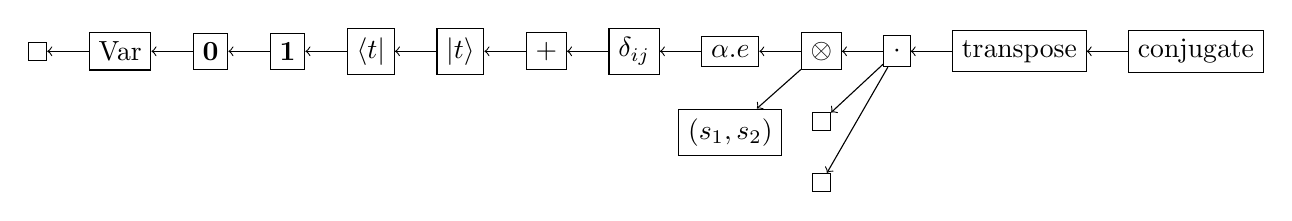
\begin{tikzpicture}[node distance=15pt]
      \node[draw]                     (tt) {$\utt$};
      \node[draw, right=of tt]         (var)   {\text{Var}};
      \node[draw, right=of var]       (zero)   {$\mathbf{0}$};
      \node[draw, right=of zero]       (id)   {$\mathbf{1}$};
      \node[draw, right=of id]       (bra) {$\bra{t}$};
      \node[draw, right=of bra]       (ket) {$\ket{t}$};
      \node[draw, right=of ket]      (add)  {$+$};
      \node[draw, right=of add]     (delta)     {$\delta_{ij}$};
      \node[draw, right=of delta]     (scaling)     {$\alpha.e$};
      \node[draw, right=of scaling]     (tensor)     {$\otimes$};
      \node[draw, right=of tensor]       (mul)  {$\cdot$};
      \node[draw, right=of mul]       (trans)     {transpose};
      \node[draw, right=of trans]     (conj)     {conjugate};

      \node[draw, below=of scaling]       (pair) {$(s_1, s_2)$};

      \node[draw, below=of tensor]       (fst)     {$\fst$};
      \node[draw, below=of fst]       (snd)     {$\snd$};

      
      \graph{
        (conj) -> (trans) -> (mul) -> (tensor) -> (scaling) -> (delta) -> (add) -> (ket) -> (bra) -> (id) -> (zero) ->(var) -> (tt);
        (tensor) -> (pair);
        (mul) -> (fst);
        (mul) -> (snd);
      };
    \end{tikzpicture}
    \end{center}

    Note that for terms with the same function symbol, the subterms are compared from right to left. Therefore, for example we have $ (a \otimes b) \otimes c <_{RPO} a \otimes (b \otimes c) $. 

\end{definition}

% \begin{lemma}
%   $<_{RPO}$ is a total order for Dirac notations in any context $\Gamma$.
% \end{lemma}

% \yx{This property must be guaranteed because it's necessary for the confluence of ordered term rewriting.}


\subsection{Reduction of Dirac Notations}

We call this term rewriting system \textsf{DN}. We use $u =_{\textsf{DN}} v$ to denote that $u$ and $v$ are equivalent in \textsf{DN}.

\subsubsection*{Pair and Projection}
\begin{align*}
  & \textsc{(Squash1)} && \Gamma \vdash (\utt, e) \reduce e 
  && \textsc{(Squash2)} && \Gamma \vdash (e, \utt) \reduce e \\
  & \textsc{(Proj1)} && \Gamma \vdash \fst\ (e_1, e_2) \reduce e_1
  && \textsc{(Proj2)} && \Gamma \vdash \snd\ (e_1, e_2) \reduce e_2  \\
  \\
  & \textsc{(Pair)} && \Gamma \vdash (\fst\ e, \snd\ e)\reduce e
  && \textsc{(Unit)} && \frac{\Gamma \vdash x : \unit \qquad x \neq \utt}{\Gamma \vdash x\reduce\utt} 
\end{align*}

\subsubsection*{Delta Expression}
\begin{align*}
  & \textsc{(DeltaZero)} && 
  \Gamma \vdash \delta_{s, t}.\mathbf{0}_{\tau, \sigma} \reduce \mathbf{0}_{\tau, \sigma}
  \\
  & \textsc{(Delta1)} && 
  \Gamma \vdash \delta_{s, s}.e \reduce e 
  \\
  \\
  & \textcolor{red}{\textsc{(Delta0)}} && 
  \frac{s =_\textsf{DN} t\ \textrm{is not satisfiable in}\ \Gamma \qquad \Gamma \vdash e : [\tau, \sigma]}{\Gamma \vdash \delta_{s, t}.e \reduce \textbf{0}_{\tau, \sigma}} \\
  \\
  & \textcolor{red}{\textsc{(DeltaDcp)}} && 
  \frac{\Gamma \vdash u : ( \tau * \sigma ) \qquad \tau \neq \unit \qquad \sigma \neq \unit}{\Gamma \vdash \delta_{u, (s, t)}.e \reduce \delta_{\fst\ u, s}.\delta_{\snd\ u, t}.e} 
  \\
  \\
  & \textsc{(DeltaPair)} &&
  \Gamma \vdash \delta_{\fst\ u, \fst\ v}.\delta_{\snd\ u, \snd\ v}.e \reduce \delta_{u, v}.e 
  \\
  & \textsc{(DeltaDist)} &&
  \Gamma \vdash \delta_{s, t}.(e_1 + e_2) \reduce \delta_{s, t}.e_1 + \delta_{s, t}.e_2
\end{align*}

\yx{$\delta_{s, t}$ is reduced to 1 when $s =_\textsf{DN} t$ is valid, and is reduced to 0 when $s =_\textsf{DN} t$ is not satisfiable. In other words, it requires to check the two terms $s$ and $t$ using the same reduction system \textsf{DN}. This is closest to the behaviour of $\delta_{s, t}$ in maths but is hard to test. I don't know whether it's appropriate.}

\textbf{Remark:} \textsc{(DeltaDcp)} does not decrease the $<_{RPO}$ order. But it should terminate because the types of $s$ and $t$ becomes simpler for $\delta_{s, t}$.

\subsubsection*{Ket}
\begin{align*}
  & \textsc{(Ket1)} && \Gamma \vdash \ket{\utt} \reduce \mathbf{1}
  && \textsc{(KetPair)} && \Gamma \vdash \ket{s} \otimes \ket{t}\reduce\ket{(s, t)} 
\end{align*}

\subsubsection*{Bra}
\begin{align*}
  & \textsc{(Bra1)} && \Gamma \vdash \bra{\utt} \reduce \mathbf{1}
  && \textsc{(BraPair)} && \Gamma \vdash \bra{s} \otimes \bra{t}\reduce\bra{(s, t)} 
\end{align*}


\subsubsection*{Conjugate}
\begin{align*}
  & \textsc{(Zero*)} && \Gamma \vdash \textbf{0}_{\tau, \sigma}^* \reduce \textbf{0}_{\tau, \sigma}
  && \textsc{(Id*)} && \Gamma \vdash \mathbf{1}^* \reduce \mathbf{1} \\
  & \textsc{(Delta*)} &&
  \Gamma \vdash (\delta_{s,t}.e)^* \reduce \delta_{s,t}.(e^*)\\
  & \textsc{(Ket*)} && \Gamma \vdash \ket{s}^* \reduce \ket{s}
  && \textsc{(Bra*)} && \Gamma \vdash \bra{s}^* \reduce \bra{s} \\
  & \textsc{(Double*)} && \Gamma \vdash (e^*)^*\reduce e
  && \textsc{(T*)} && \Gamma \vdash (e^\top)^* \reduce(e^*)^\top \\
  & \textsc{(Scr*)} && \Gamma \vdash (\alpha.e)^* \reduce (\alpha^*).(e^*) \\
  & \textsc{(Add*)} && \Gamma \vdash (e_1 + e_2)^* \reduce e_1^* + e_2^* 
  && \textsc{(Mul*)} && \Gamma \vdash (e_1 \cdot e_2)^* \reduce e_1^* \cdot e_2^* \\
  & \textsc{(Tsr*)} && \Gamma \vdash (e_1 \otimes e_2)^* \reduce e_1^* \otimes e_2^*
\end{align*}

\subsubsection*{Transpose}
\begin{align*}
  & \textsc{(ZeroT)} && \Gamma \vdash \textbf{0}_{\tau, \sigma}^\top \reduce \textbf{0}_{\sigma, \tau}
  && \textsc{(IdT)} && \Gamma \vdash \mathbf{1}^\top \reduce \mathbf{1} \\
  & \textsc{(DeltaT)} && \Gamma \vdash (\delta_{s,t}.e)^\top \reduce \delta_{s,t}.(e^\top) \\
  & \textsc{(KetT)} && \Gamma \vdash \ket{s}^\top \reduce \bra{s} 
  && \textsc{(BraT)} && \Gamma \vdash \bra{s}^\top \reduce \ket{s} \\
  & \textsc{(DoubleT)} && \Gamma \vdash (e^\top)^\top \reduce e 
  && \textsc{(ScrT)} && \Gamma \vdash (\alpha.e)^\top \reduce \alpha.(e^\top) \\
  & \textsc{(AddT)} && \Gamma \vdash (e_1 + e_2)^\top \reduce e_1^\top + e_2^\top
  && \textsc{(MulT)} && \Gamma \vdash (e_1 \cdot e_2)^\top \reduce e_2^\top \cdot e_1^\top \\
  & \textsc{(TsrT)} && \Gamma \vdash (e_1 \otimes e_2)^\top \reduce e_1^\top \otimes e_2^\top
\end{align*}

\subsubsection*{Scaling}
\begin{align*}
  & \textcolor{red}{\textsc{(Scr0)}} && \frac{\Gamma \vdash e : [\tau, \sigma]}{\Gamma \vdash 0.e \reduce \textbf{0}_{\tau, \sigma}}
  && \textsc{(Scr1)} && \Gamma \vdash 1.e \reduce e \\
  \\
  & \textsc{(ScrZero)} && \Gamma \vdash \alpha.\mathbf{0}_{\tau, \sigma} \reduce \mathbf{0}_{\tau, \sigma}
  && \textsc{(ScrDelta)} && \Gamma \vdash \alpha.\delta_{s, t}.e \reduce \delta_{s, t}.\alpha.e \\
  & \textsc{(ScrScr)} && \Gamma \vdash \alpha.\beta.e \reduce (\alpha \times \beta).e
  \\
  & \textsc{(ScrDist)} && \Gamma \vdash \alpha.(e_1 + e_2) \reduce \alpha.e_1 + \alpha.e_2
\end{align*}

\subsubsection*{Addition}
\begin{align*}
  & \textsc{(AddZero)} && \Gamma \vdash e + \textbf{0}_{\tau, \sigma} \reduce e \\
  & \textcolor{red}{\textsc{(Fac2)}} && 
    \Gamma \vdash \alpha.e + \beta.e \reduce (\alpha + \beta).e
  && \textcolor{red}{\textsc{(Fac1)}} &&
    \Gamma \vdash \alpha.e + e \reduce (\alpha + 1).e \\
  & \textcolor{red}{\textsc{(Fac0)}} &&
    \Gamma \vdash e + e \reduce (1 + 1).e
\end{align*}

\yx{These three factorization rules does not decrease the $<_{RPO}$ order. I should consult the Lineal paper and see how they handled this. }

\subsubsection*{Multiplication}
\begin{align*}
  & \textcolor{red}{\textsc{(MulZeroL)}}
  && \frac{\Gamma \vdash e : [\tau, \rho]}{\Gamma \vdash \textbf{0}_{\rho, \sigma} \cdot e \reduce \textbf{0}_{\tau, \sigma}}
  && \textcolor{red}{\textsc{(MulZeroR)}}
  && \frac{\Gamma \vdash e : [\rho, \sigma]}{\Gamma \vdash e \cdot \textbf{0}_{\tau, \rho} \reduce \textbf{0}_{\tau, \sigma}} \\
  \\
  & \textsc{(MulIdL)} && \Gamma \vdash \mathbf{1} \cdot e \reduce e 
  && \textsc{(MulIdR)} && \Gamma \vdash e \cdot \mathbf{1} \reduce e 
  \\
  & \textsc{(MulScrL)} && \Gamma \vdash (\alpha.u) \cdot v \reduce \alpha.(u \cdot v)
  && \textsc{(MulScrR)} && \Gamma \vdash u \cdot (\alpha.v) \reduce \alpha.(u \cdot v)
  \\
  & \textsc{(MulDeltaL)} && \Gamma \vdash (\delta_{s, t}.u) \cdot v \reduce \delta_{s, t}.(u \cdot v)
  && \textsc{(MulDeltaR)} && \Gamma \vdash u \cdot (\delta_{s, t}.v) \reduce \delta_{s, t}.(u \cdot v)
  \\
  & \textsc{(MulBraKet)} && \Gamma \vdash \bra{s} \cdot \ket{t} \reduce \delta_{s, t}.\mathbf{1} \\ 
  & \textsc{(MulDistL)} && \Gamma \vdash (u + v) \cdot e \reduce u \cdot e + v \cdot e
  && \textsc{(MulDistR)} && \Gamma \vdash e \cdot (u + v) \reduce e \cdot u + e \cdot v \\
  \\
  & \textsc{(ReFac2)} && \frac{\Gamma \vdash a_1 : [\rho, \tau] \qquad \Gamma \vdash b_1 : [\sigma, \rho]}{\Gamma \vdash (a_1 \otimes a_2) \cdot (b_1 \otimes b_2) \reduce (a_1 \cdot b_1) \otimes (a_2 \cdot b_2)} \\
\end{align*}

\begin{align*}
  & \textsc{(ReFac1LL)} && \frac{\Gamma \vdash e : [\unit, \tau]}{\Gamma \vdash (e \otimes a) \cdot b \reduce e \otimes (a \cdot b)}
  && \textsc{(ReFac1LR)} && \frac{\Gamma \vdash e : [\unit, \tau]}{\Gamma \vdash (a \otimes e) \cdot b \reduce (a \cdot b) \otimes e} \\
  \\
  & \textsc{(ReFac1RL)} && \frac{\Gamma \vdash e : [\tau, \unit]}{\Gamma \vdash a \cdot (e \otimes b) \reduce e \otimes (a \cdot b)} 
  && \textsc{(ReFac1RR)} && \frac{\Gamma \vdash e : [\tau, \unit]}{\Gamma \vdash a \cdot (b \otimes e) \reduce (a \cdot b) \otimes e} \\
  \\
  & \textsc{(ReFac0)} && \frac{\Gamma \vdash a : [\unit, \tau] \qquad \Gamma \vdash b : [\sigma, \unit]}{\Gamma \vdash a \cdot b \reduce a \otimes b}
\end{align*}

\begin{align*}
  & \textsc{(ReFacBPair)} && \frac{\Gamma \vdash u : (\tau * \sigma) \qquad \tau \neq \unit \qquad \sigma \neq \unit \qquad \Gamma \vdash a : [\rho, \tau]}{\Gamma \vdash \bra{u} \cdot (a \otimes b) \reduce (\bra{\fst\ u} \cdot a) \otimes (\bra{\snd\ u} \cdot b)} \\
  \\
  & \textsc{(ReFacKPair)} && \frac{\Gamma \vdash u : (\tau * \sigma) \qquad \tau \neq \unit \qquad \sigma \neq \unit \qquad \Gamma \vdash a : [\sigma, \rho]}{\Gamma \vdash (a \otimes b) \cdot \ket{u}  \reduce (a \cdot \ket{\fst\ u}) \otimes (b \cdot \ket{\snd\ u})}
\end{align*}
% \textbf{Remark: } The last several rules conduct \textbf{tensorization}. They have clear tensor network interpretations. 
% And also, the procedure of tensorization is actually optimizing the contraction order of the tensor network.


\subsubsection*{Tensor}
\begin{align*}
  & \textcolor{red}{\textsc{(TsrZeroL)}} && 
  \frac{\Gamma \vdash e : [\tau, \sigma]}{\Gamma \vdash \textbf{0}_{\tau', \sigma'} \otimes e \reduce \textbf{0}_{(\tau' * \tau), (\sigma' * \sigma)}} 
  && \textcolor{red}{\textsc{(TsrZeroR)}} && 
  \frac{\Gamma \vdash e : [\tau, \sigma]}{\Gamma \vdash e \otimes \textbf{0}_{\tau', \sigma'} \reduce \textbf{0}_{(\tau * \tau'), (\sigma * \sigma')}} \\
  & \textsc{(TsrIdL)} && 
  \Gamma \vdash \mathbf{1} \otimes e \reduce e
  && \textsc{(TsrIdR)} && 
  \Gamma \vdash e \otimes \mathbf{1} \reduce e
  \\
  & \textsc{(TsrScrL)} && \Gamma \vdash (\alpha.u) \otimes v \reduce \alpha.(u \otimes v) 
  && \textsc{(TsrScrR)} && \Gamma \vdash u \otimes (\alpha.v) \reduce \alpha.(u \otimes v)
  \\
  & \textsc{(TsrDeltaL)} && \Gamma \vdash (\delta_{s, t}.u) \otimes v \reduce \delta_{s, t}.(u \otimes v) 
  && \textsc{(TsrDeltaR)} && \Gamma \vdash u \otimes (\delta_{s, t}.v) \reduce \delta_{s, t}.(u \otimes v)
  \\
  & \textsc{(TsrDistL)} && \Gamma \vdash (u + v) \otimes e \reduce u \otimes e + v \otimes e
  && \textsc{(TsrDistR)} && \Gamma \vdash e \otimes (u + v) \reduce e \otimes u + e \otimes v
\end{align*}
  
\begin{align*}
  & \textsc{(TsrSort0)} && 
  \frac{
    \begin{aligned}
      & \Gamma \vdash u : [\tau_u, \sigma_u] \qquad \Gamma \vdash v_i : [\tau_{v_i}, \sigma_{v_i}] \\
      & \tau_u = \unit \vee \bigwedge_{i = 1}^n \tau_{v_i} = \unit \qquad \sigma_u = \unit \vee \bigwedge_{i = 1}^n \sigma_{v_i} = \unit
    \end{aligned} 
    \qquad 
    \qquad u <_{RPO} v_n
    }{\Gamma \vdash u \otimes v_1 \otimes \cdots \otimes v_n \reduce v_i \otimes \cdots \otimes v_n \otimes u} \\
  \\
  & \textsc{(TsrSort1)} && 
  \frac{
    \begin{aligned}
      & \Gamma \vdash u : [\tau_u, \sigma_u] \qquad \Gamma \vdash v_i : [\tau_{v_i}, \sigma_{v_i}] \\
      & \tau_u = \unit \vee \bigwedge_{i = 1}^n \tau_{v_i} = \unit \qquad \sigma_u = \unit \vee \bigwedge_{i = 1}^n \sigma_{v_i} = \unit
    \end{aligned} 
    \qquad 
    \qquad u <_{RPO} v_n
    }{\Gamma \vdash e \otimes u \otimes v_1 \otimes \cdots \otimes v_n \reduce e \otimes v_i \otimes \cdots \otimes v_n \otimes u} \\
  \\
  & \textsc{(TsrAssoc)} &&
  \frac{
    \begin{aligned}
      & \Gamma \vdash u : [\tau_u, \sigma_u] \qquad \Gamma \vdash v : [\tau_v, \sigma_v] \qquad \Gamma \vdash w : [\tau_w, \sigma_w] \\
      & \tau_u = \unit \vee \tau_v = \unit \vee \tau_w = \unit \qquad \sigma_u = \unit \vee \sigma_v = \unit \vee \sigma_w = \unit
    \end{aligned}
    }{\Gamma \vdash u \otimes (v \otimes w) \reduce u \otimes v \otimes w}
\end{align*}

\yx{Because there are some restrictions on swapping the order of tensoring, we have to incorporate special rules \textsc{(TsrSort0)} and \textsc{(TsrSort1)}. Common commutative and associative rules are not enough for confluence. I don't know whether this is appropriate.}
\\

\yx{The rules in red does not follow the $<_{RPO}$.
\begin{enumerate}
  \item Conflict in the order of function symbols $\alpha.e$ and $e + e$, due to the existence of factorization rules and distribution rules.
  \item problem of $\mathbf{0}_{\tau, \sigma}$: the types $\tau$ and $\sigma$ do not appear as subterms in the LHS of the rule. (Maybe we can ignore the type hints for zero operator)
\end{enumerate}
}

\begin{lemma}[preservation of Dirac types]
  For any context $\Gamma$ and terms $e, e'$, if $\Gamma \vdash e : \tau$ and $\Gamma \vdash e \reduce e'$, we have
  $ \Gamma \vdash e' : \tau $. 
\end{lemma}
\begin{proof}
  By case analysis. It's worth noting that tensoring scalar-like notations will not change the type, becuase $(\unit * \tau) = \tau$ by the equational theory.
\end{proof}

\subsection{Termination and Confluence}

\begin{lemma}[termination]
  The reduction system is terminating. In other words, for any context $\Gamma$ and a well-typed expression $\Gamma \vdash e : \tau$, there does not exists an infinite reduction $\Gamma \vdash e \reduce e' \reduce\cdots .$
\end{lemma}
\begin{proof}
  \yx{TO BE PROVED. Outline: for rules that do not decrease $<_{RPO}$, we prove they are terminating (on all terms matching their LHS). Then combined with the fact that $<_{RPO}$ is a well-founded order, we can conclude that the whole system is terminating.
  I don't know whether this works. More consideration needed.}
\end{proof}


\begin{lemma}[convergence]
  The reduction system is convergent. In other words, for any context $\Gamma$ and a well-typed expression $\Gamma \vdash e : \tau$, all reduction sequence from it are finite and end in the unique normal form for $e$.
\end{lemma}
\begin{proof}
  Since the reduction system is terminating, we only need to check that all the critical pairs are joinable. Here is a thorough list of them:
  \begin{itemize}
    %%%%%%%%%%%%%%%%%%%%%%%%%%%%%%%%%%%%%%%%%%%%%%%%%%%%%%%%%%%%%%%%%%
    \item \textbf{critical pairs containing} \textsc{(Squash1)}/\textsc{(Squash2)} 
    
      \begin{flalign*}
        & (\utt, \utt) \reduce \left \{
          \begin{aligned}
            & \textsc{(Squash1)} && \\
            & \textsc{(Squash2)} &&
          \end{aligned}
        \right \} \reduce \utt &
      \end{flalign*}

      \textbf{Remark:} There is no critical pairs between \textsc{(Squash1)-(DeltaDcp)}: $\delta_{u, (\utt, t)}.e$ does not satisfy the side condition of \textsc{(DeltaDcp)}. Similar for \textsc{(Squash2)-(DeltaDcp)}.

      %%%%%%%%%%%%%%%%%%%%%%%%%%%%%%%%%%%%%%%%%%%%%%%%%%%%%%%%%%%%%%%%%%
      \item \textbf{critical pairs containing} \textsc{(Proj1)}/\textsc{(Proj2)}
      \begin{flalign*}
        & (\fst\ (e_1, e_2), \snd\ (e_1, e_2)) \reduce \left \{
          \begin{aligned}
            & \textsc{(Proj1)} && (e_1, \snd\ (e_1, e_2)) \\
            & \textsc{(Pair)} &&
          \end{aligned}
        \right \} \reduce (e_1, e_2) &
      \end{flalign*}
      \textbf{Remark:} Similar for the \textsc{(Proj2)-(Pair)} pair from $(\fst\ (e_1, e_2), \snd\ (e_1, e_2))$.

      \begin{flalign*}
        & \delta_{\fst\ (a, b), \fst\ u}.\delta_{\snd\ (a, b), \snd\ u}.e \reduce \left \{
          \begin{aligned}
            & \textsc{(Proj1)} && \delta_{a, \fst\ u}.\delta_{\snd\ (a, b), \snd\ u}.e  \\
            & \textsc{(DeltaPair)} && \delta_{(a, b), u}.e 
          \end{aligned}
        \right \} \reduce \delta_{a, \fst\ u}.\delta_{b, \snd\ u}.e &
      \end{flalign*}
      \textbf{Remark:} Similar for the \textsc{(Proj2)-(DeltaPair)} pair from $\delta_{\fst\ (a, b), \fst\ u}.\delta_{\snd\ (a, b), \snd\ u}.e$.


      %%%%%%%%%%%%%%%%%%%%%%%%%%%%%%%%%%%%%%%%%%%%%%%%%%%%%%%%%%%%%%%%%%
      \item \textbf{critical pairs containing} \textsc{(Pair)}
      \begin{flalign*}
        & \delta_{u, (\fst\ v, \snd\ v)}.e \reduce \left \{
          \begin{aligned}
            & \textsc{(Pair)} && \\
            & \textsc{(DeltaDcp)} && \delta_{\fst\ u, \fst\ v}.\delta_{\snd\ u, \snd\ v}.e
          \end{aligned}
        \right \} \reduce \delta_{u, v}.e &
      \end{flalign*}



    %%%%%%%%%%%%%%%%%%%%%%%%%%%%%%%%%%%%%%%%%%%%%%%%%%%%%%%%%%%%%%%%%%
    \item \textbf{critical pairs containing} \textsc{(DeltaZero)}
     
      These critical pairs always join at the zero operator and are all trival.

    %%%%%%%%%%%%%%%%%%%%%%%%%%%%%%%%%%%%%%%%%%%%%%%%%%%%%%%%%%%%%%%%%%
    \item \textbf{critical pairs containing} \textsc{(Delta1)}

      \begin{flalign*}
        & \delta_{(s, t), (s, t)}.e \reduce \left \{
          \begin{aligned}
            & \textsc{(Delta1)} && \\
            & \textsc{(DeltaDcp)} && \delta_{\fst\ (s, t), s}.\delta_{\snd\ (s, t), t}.e \reduce \delta_{s, s}.\delta_{t, t}.e
          \end{aligned}
        \right \} \reduce e &
      \end{flalign*}

      \begin{flalign*}
        & \delta_{\fst\ u, \fst\ u}.\delta_{\snd\ u, \snd\ u}.e \reduce \left \{
          \begin{aligned}
            & \textsc{(Delta1)} && \\
            & \textsc{(DeltaPair)} && \delta_{u, u}.e
          \end{aligned}
        \right \} \reduce e &
      \end{flalign*}

      \begin{flalign*}
        & \delta_{s, s}.(e_1 + e_2) \reduce \left \{
          \begin{aligned}
            & \textsc{(Delta1)} && \\
            & \textsc{(DeltaDist)} && \delta_{s, s}.e_1 + \delta_{s, s}.e_2
          \end{aligned}
        \right \} \reduce e_1 + e_2 &
      \end{flalign*}
      \textbf{Remark:} Other critical pairs are trival:
      \begin{itemize}
        \item \textsc{(Delta1)-(Delta*)} pair from $(\delta_{s, s}.e)^*$,
        \item \textsc{(Delta1)-(DeltaT)} pair from $(\delta_{s, s}.e)^\top$,
        \item \textsc{(Delta1)-(ScrDelta)} pair from $\alpha.\delta_{s, s}.e$,
        \item \textsc{(Delta1)-(MulDeltaL)} pair from $(\delta_{s, s}.u) \cdot v$,
        \item \textsc{(Delta1)-(MulDeltaR)} pair from $u \cdot (\delta_{s, s}.v)$,
        \item \textsc{(Delta1)-(TsrDeltaL)} pair from $(\delta_{s, s}.u) \otimes v$, and
        \item \textsc{(Delta1)-(TsrDeltaR)} pair from $u \otimes (\delta_{s, s}.v)$.
      \end{itemize}


    %%%%%%%%%%%%%%%%%%%%%%%%%%%%%%%%%%%%%%%%%%%%%%%%%%%%%%%%%%%%%%%%%%
    \item \textbf{critical pairs containing} \textsc{(Delta0)}

      \begin{flalign*}
        & \delta_{u, (s, t)}.e \reduce \left \{
          \begin{aligned}
            & \textsc{(Delta0)} && \\
            & \textsc{(DeltaDcp)} && \delta_{\fst\ u, s}.\delta_{\snd\ u, t}.e \reduce \cdots
          \end{aligned}
        \right \} \reduce \textbf{0}_{\tau, \sigma} \\
        & \text{($u =_\textsf{DN} (s, t)$ is not satisfiable, $\Gamma \vdash e : [\tau, \sigma]$)} &
      \end{flalign*}
      \textbf{Remark:} If $u =_\textsf{DN} (s, t)$ is not satisfiable, then either $\fst\ u =_\textsf{DN} s$ or $\snd\ u =_\textsf{DN} t$ is not satisfiable. Therefore the expression will always be reduced to $\textbf{0}$.  
    
      \begin{flalign*}
        & \delta_{\fst\ u, \fst\ v}.\delta_{\snd\ u, \snd\ v}.e \reduce \left \{
          \begin{aligned}
            & \textsc{(Delta0)} && \\
            & \textsc{(DeltaPair)} && \delta_{u, v}.e
          \end{aligned}
        \right \} \reduce \textbf{0}_{\tau, \sigma} \\
        & \text{($\fst\ u =_\textsf{DN} \fst\ v$ is not satisfiable, $\Gamma \vdash e : [\tau, \sigma]$)} &
      \end{flalign*}
      \textbf{Remark:} If $\fst\ u =_\textsf{DN} \fst\ v$ is not satisfiable, then $u =_\textsf{DN} v$ is not satisfiable.

    \textbf{Remark:} Other critical pairs are trival:
    \begin{itemize}
      \item \textsc{(Delta0)-(DeltaDist)} pair from $\delta_{s, t}.(e_1 + e_2)$,
      \item \textsc{(Delta0)-(Delta*)} pair from $(\delta_{s, t}.e)^*$,
      \item \textsc{(Delta0)-(DeltaT)} pair from $(\delta_{s, t}.e)^\top$,
      \item \textsc{(Delta0)-(ScrDelta)} pair from $\alpha.\delta_{s, t}.e$,
      \item \textsc{(Delta0)-(MulDeltaL)} pair from $(\delta_{s, t}.u) \cdot v$,
      \item \textsc{(Delta0)-(MulDeltaR)} pair from $u \cdot (\delta_{s, t}.v)$,
      \item \textsc{(Delta0)-(TsrDeltaL)} pair from $(\delta_{s, t}.u) \otimes v$, and
      \item \textsc{(Delta0)-(TsrDeltaR)} pair from $u \otimes (\delta_{s, t}.v)$.
    \end{itemize}

    %%%%%%%%%%%%%%%%%%%%%%%%%%%%%%%%%%%%%%%%%%%%%%%%%%%%%%%%%%%%%%%%%%
    \item \textbf{critical pairs containing} \textsc{(DeltaDcp)}
      \begin{flalign*}
        & \delta_{(a, b), (u, v)}.e \reduce \left \{
          \begin{aligned}
            & \textsc{(DeltaDcp)} && \delta_{\fst\ (a, b), u}.\delta_{\snd\ (a, b), v}.e \\
            & \textsc{(DeltaDcp)} && \delta_{a, \fst\ (u, v)}.\delta_{b, \snd\ (u, v)}.e
          \end{aligned}
        \right \} \reduce \delta_{a, u}.\delta_{b, v}.e &
      \end{flalign*}

      \textbf{Remark:} Other critical pairs are trival.

    %%%%%%%%%%%%%%%%%%%%%%%%%%%%%%%%%%%%%%%%%%%%%%%%%%%%%%%%%%%%%%%%%%
    \item \textbf{critical pairs containing} \textsc{(DeltaPair)}
    
    No extra critical pairs.
    % \begin{flalign*}
    %   & \delta_{\fst\ u, \fst\ v}.\delta_{\snd\ u, \snd\ v}.\delta_{\fst\ u, \fst\ v}.e \reduce \left \{
    %     \begin{aligned}
    %       & \textsc{(DeltaPair)} && \delta_{u, v}.\delta_{\fst\ u, \fst\ v}.e \\
    %       & \textsc{(DeltaPair)} && \delta_{\fst\ u, \fst\ v}.\delta_{u, v}.e
    %     \end{aligned}
    %   \right \} \reduce \delta_{u, v}.\delta_{\fst\ u, \fst\ v}.e &
    % \end{flalign*}
    % \textbf{Remark:} Similar for another critical pair from $\delta_{\fst\ u, \fst\ v}.\delta_{\snd\ u, \snd\ v}.\delta_{\snd\ u, \snd\ v}.e$.
    
    %%%%%%%%%%%%%%%%%%%%%%%%%%%%%%%%%%%%%%%%%%%%%%%%%%%%%%%%%%%%%%%%%%
    \item \textbf{critical pairs containing} \textsc{(DeltaDist)}
    
    All critical pairs are trivial.
  
    %%%%%%%%%%%%%%%%%%%%%%%%%%%%%%%%%%%%%%%%%%%%%%%%%%%%%%%%%%%%%%%%
    \item \textbf{critical pairs containing} \textsc{(Ket1)}/\textsc{(Bra1)}
    
    Here we present all the critical pairs involves ket $\ket{\utt}$. Those for bra $\bra{\utt}$ are totally symmetric.

      \begin{flalign*}
        & \ket{\utt} \otimes \ket{s} \reduce \left \{
          \begin{aligned}
            & \textsc{(Ket1)} && \mathbf{1} \otimes \ket{s} \\
            & \textsc{(KetPair)} && \ket{(\utt, s)}
          \end{aligned}
        \right \} \reduce \ket{s} &
      \end{flalign*}
      \textbf{Remark:} Similar for the \textsc{(Ket1)-(KetPair)} from $\ket{s} \otimes \ket{\utt}$.

      \begin{flalign*}
        & \ket{\utt}^* \reduce \left \{
          \begin{aligned}
            & \textsc{(Ket1)} && \mathbf{1}^* \\
            & \textsc{(Ket*)} && \ket{\utt}
          \end{aligned}
        \right \} \reduce \mathbf{1} &
      \end{flalign*}

      \begin{flalign*}
        & \ket{\utt}^\top \reduce \left \{
          \begin{aligned}
            & \textsc{(Ket1)} && \mathbf{1}^\top \\
            & \textsc{(KetT)} && \bra{\utt}
          \end{aligned}
        \right \} \reduce \mathbf{1} &
      \end{flalign*}

      \begin{flalign*}
        & \bra{s} \cdot \ket{\utt} \reduce \left \{
          \begin{aligned}
            & \textsc{(Ket1)}&& \bra{s} \cdot \mathbf{1} \reduce \bra{\utt} \cdot \mathbf{1} \reduce \mathbf{1} \cdot \mathbf{1} \\
            & \textsc{(MulBraKet)} && \delta_{s, \utt}.\mathbf{1} \reduce \delta_{\utt, \utt}.\mathbf{1}
          \end{aligned}
        \right \} \reduce \mathbf{1} &
      \end{flalign*}
      \textbf{Remark:} $\Gamma \vdash s : \unit$ holds in this case. 

  %%%%%%%%%%%%%%%%%%%%%%%%%%%%%%%%%%%%%%%%%%%%%%%%%%%%%%%%%%%%%%%%
  \item \textbf{critical pairs containing} \textsc{(KetPair)}/\textsc{(BraPair)}
  
  Here we present all the critical pairs involves ket $\ket{s} \otimes \ket{t}$. Those for bra $\bra{s} \otimes \bra{t}$ are totally symmetric.

  \begin{flalign*}
      & (\ket{s} \otimes \ket{t})^* \reduce \left \{
        \begin{aligned}
          & \textsc{(KetPair)} && \ket{(s, t)}^* \\
          & \textsc{(Tsr*)} && \ket{s}^* \otimes \ket{t}^* \reduce \ket{s} \otimes \ket{t}
        \end{aligned}
      \right \} \reduce \ket{(s, t)} &
    \end{flalign*}

    \begin{flalign*}
      & (\ket{s} \otimes \ket{t})^\top \reduce \left \{
        \begin{aligned}
          & \textsc{(KetPair)} && \ket{(s, t)}^\top \\
          & \textsc{(TsrT)} && \ket{s}^\top \otimes \ket{t}^\top \reduce \bra{s} \otimes \bra{t}
        \end{aligned}
      \right \} \reduce \bra{(s, t)} &
    \end{flalign*}

    \begin{flalign*}
      & (a \otimes b) \cdot (\ket{s} \otimes \ket{t}) \reduce \left \{
        \begin{aligned}
          & \textsc{(KetPair)} && (a \otimes b) \cdot \ket{(s, t)} \\
          & \textsc{(ReFac2)} && 
        \end{aligned}
      \right \} \reduce (a \cdot \ket{s}) \otimes (b \cdot \ket{t}) \\
      & (\Gamma \vdash a : [\rho, \tau], \Gamma \vdash \ket{s} : [\unit, \rho]) &
    \end{flalign*}

    %%%%%%%%%%%%%%%%%%%%%%%%%%%%%%%%%%%%%%%%%%%%%%%%%%%%%%%%%%%%%%%%
    \item \textbf{conjugate critical pairs}    
    
      \begin{flalign*}
      & (\mathbf{0}_{\tau, \sigma}^*)^* \reduce \left \{
        \begin{aligned}
          & \textsc{(Double*)} && \\
          & \textsc{(Zero*)} && (\mathbf{0}_{\tau, \sigma})^* 
        \end{aligned}
        \right \} \reduce \mathbf{0}_{\tau, \sigma}&
      \end{flalign*}
      \textbf{Remark:} Similar for $((\mathbf{1})^*)^*$, $((\delta_{s, t}.e)^*)^*$, $(\ket{s}^*)^*$ and $(\bra{s}^*)^*$.
      
      \begin{flalign*}
        & ((\alpha.e)^*)^* \reduce \left \{
          \begin{aligned}
            & \textsc{(Double*)} && \\
            & \textsc{(C*)} && ((\alpha^*).e^*)^* \reduce ((\alpha^*)^*).e 
          \end{aligned}
        \right \} \reduce \alpha.e &
      \end{flalign*}

      \begin{flalign*}
        & ((e^*)^*)^* \reduce \left \{
          \begin{aligned}
            & \textsc{(Double*)} && \\
            & \textsc{(Double*)} &&
          \end{aligned}
        \right \} \reduce e^* &
      \end{flalign*}
      \textbf{Remark:} The \textsc{(Double*)} rule can overlap with itself.

      \begin{flalign*}
        & ((e^\top)^*)^* \reduce \left \{
          \begin{aligned}
            & \textsc{(Double*)} && \\
            & \textsc{(T*)} && ((e^*)^\top)^* \reduce ((e^*)^*)^\top 
          \end{aligned}
        \right \} \reduce e^\top &
      \end{flalign*}

      \begin{flalign*}
        & ((e_1 + e_2)^*)^* \reduce \left \{
          \begin{aligned}
            & \textsc{(Double*)} && \\
            & \textsc{(Add*)} && (e_1^* + e_2^*)^* \reduce (e_1^*)^* + (e_2^*)^*
          \end{aligned}
        \right \} \reduce e_1 + e_2 &
      \end{flalign*}
      \textbf{Remark:} Similar for $((e_1 \cdot e_2)^*)^*$, $((e_1 \otimes e_2)^*)^*$.

    %%%%%%%%%%%%%%%%%%%%%%%%%%%%%%%%%%%%%%%%%%%%%%%%%%%%%%%%%%%%%%%%
    \item \textbf{transpose critical pairs}
    
      The critical pairs related to transpose reduction rules are similar to those of conjugate.

    %%%%%%%%%%%%%%%%%%%%%%%%%%%%%%%%%%%%%%%%%%%%%%%%%%%%%%%%%%%%%%%%
    \item \textbf{critical pairs containing} \textsc{(Scr0)}
    
      \begin{flalign*}
        & 0.\mathbf{0}_{\tau, \sigma} \reduce \left \{
          \begin{aligned}
            & \textsc{(Scr0)} && \\
            & \textsc{(ScrZero)} && 
          \end{aligned}
        \right \} \reduce \mathbf{0}_{\tau, \sigma} &
      \end{flalign*}

      \begin{flalign*}
        & 0.\delta_{s, t}.e \reduce \left \{
          \begin{aligned}
            & \textsc{(Scr0)} && \\
            & \textsc{(ScrDelta)} && \delta_{s, t}.0.e \reduce \delta_{s, t}.\mathbf{0}_{\tau, \sigma}
          \end{aligned}
        \right \} \reduce \mathbf{0}_{\tau, \sigma} \qquad (\Gamma \vdash e : [\tau, \sigma]) &
      \end{flalign*}

      \begin{flalign*}
        & 0.\alpha.e \reduce \left \{
          \begin{aligned}
            & \textsc{(Scr0)} && \\
            & \textsc{(ScrScr)} && (0 \times \alpha).e
          \end{aligned}
        \right \} \reduce \mathbf{0}_{\tau, \sigma} \qquad (\Gamma \vdash e : [\tau, \sigma]) &
      \end{flalign*}

      \begin{flalign*}
        & 0.(e_1 + e_2) \reduce \left \{
          \begin{aligned}
            & \textsc{(Scr0)} && \\
            & \textsc{(ScrDist)} && 0.e_1 + 0.e_2 \reduce \mathbf{0}_{\tau, \sigma} + 0.e_2 \reduce \mathbf{0}_{\tau, \sigma} + \mathbf{0}_{\tau, \sigma}
          \end{aligned}
        \right \} \reduce \mathbf{0}_{\tau, \sigma} \qquad (\Gamma \vdash (e_1 + e_2) : [\tau, \sigma]) &
      \end{flalign*}

      \begin{flalign*}
        & 0.e + \beta.e \reduce \left \{
          \begin{aligned}
            & \textsc{(Scr0)} && \mathbf{0}_{\tau, \sigma} + \beta.e \\
            & \textsc{(Fac2)} && (0 + \beta).e
          \end{aligned}
        \right \} \reduce \beta.e \qquad (\Gamma \vdash e : [\tau, \sigma]) &
      \end{flalign*}
      \textbf{Remark:} Similar for the \textsc{(Scr0)-(Fac1)} pair from $0.e + e$

      \begin{flalign*}
        & (0.u) \cdot v \reduce \left \{
          \begin{aligned}
            & \textsc{(Scr0)} && \mathbf{0}_{\tau, \sigma} \cdot v \\
            & \textsc{(MulScrL)} && 0.(u \cdot v)
          \end{aligned}
        \right \} \reduce \mathbf{0}_{\rho, \sigma} \qquad (\Gamma \vdash u : [\tau, \sigma], \Gamma \vdash v : [\rho, \tau]) &
      \end{flalign*}
      \textbf{Remark:} Similar for the \textsc{(Scr0)-(MulScrR)} pair from $u \cdot (0.v)$, the \textsc{(Scr0)-(TsrScrL)} pair from $(0.u) \otimes v$ and the \textsc{(Scr0)-(TsrScrR)} pair from $u \otimes (0.v)$.

    %%%%%%%%%%%%%%%%%%%%%%%%%%%%%%%%%%%%%%%%%%%%%%%%%%%%%%%%%%%%%%%%
    \item \textbf{critical pairs containing} \textsc{(Scr1)}
      
      \begin{flalign*}
        & 1.\mathbf{0}_{\tau, \sigma} \reduce \left \{
          \begin{aligned}
            & \textsc{(Scr1)} && \\
            & \textsc{(ScrZero)} && 
          \end{aligned}
        \right \} \reduce \mathbf{0}_{\tau, \sigma} &
      \end{flalign*}


      \begin{flalign*}
        & 1.\delta_{s, t}.e \reduce \left \{
          \begin{aligned}
            & \textsc{(Scr1)} && \\
            & \textsc{(ScrDelta)} && \delta_{s, t}.1.e
          \end{aligned}
        \right \} \reduce \delta_{s, t}.e &
      \end{flalign*}

      \begin{flalign*}
        & 1.\alpha.e \reduce \left \{
          \begin{aligned}
            & \textsc{(Scr1)} && \\
            & \textsc{(ScrScr)} && (1 \times \alpha).e
          \end{aligned}
        \right \} \reduce \alpha.e &
      \end{flalign*}

      \begin{flalign*}
        & 1.(e_1 + e_2) \reduce \left \{
          \begin{aligned}
            & \textsc{(Scr1)} && \\
            & \textsc{(ScrDist)} && 1.e_1 + 1.e_2 \reduce e_1 + 1.e_2
          \end{aligned}
        \right \} \reduce e_1 + e_2 &
      \end{flalign*}

      \begin{flalign*}
        & 1.e + \beta.e \reduce \left \{
          \begin{aligned}
            & \textsc{(Scr1)} && e + \beta.e \\
            & \textsc{(Fac2)} && 
          \end{aligned}
        \right \} \reduce (1 + \beta).e &
      \end{flalign*}
      \textbf{Remark:} Similar for the \textsc{(Scr1)-(Fac1)} pair from $1.e + e$.

      \begin{flalign*}
        & (1.u) \cdot v \reduce \left \{
          \begin{aligned}
            & \textsc{(Scr1)} && \\
            & \textsc{(MulScrL)} && 1.(u \cdot v)
          \end{aligned}
        \right \} \reduce u \cdot v &
      \end{flalign*}
      \textbf{Remark:} Similar for the \textsc{(Scr1)-(MulScrR)} pair from $u \cdot (1.v)$, the \textsc{(Scr1)-(TsrScrL)} pair from $(1.u) \otimes v$ and the \textsc{(Scr1)-(TsrScrR)} pair from $u \otimes (1.v)$.

    %%%%%%%%%%%%%%%%%%%%%%%%%%%%%%%%%%%%%%%%%%%%%%%%%%%%%%%%%%%%%%%%
    \item \textbf{critical pairs containing} \textsc{(ScrZero)}

      \begin{flalign*}
        & \alpha.\mathbf{0}_{\tau, \sigma} + \beta.\mathbf{0}_{\tau, \sigma} \reduce \left \{
          \begin{aligned}
            & \textsc{(ScrZero)} && \mathbf{0}_{\tau, \sigma} + \beta.\mathbf{0}_{\tau, \sigma} \reduce \mathbf{0}_{\tau, \sigma} + \mathbf{0}_{\tau, \sigma} \\
            & \textsc{(Fac2)} && (\alpha + \beta). \mathbf{0}_{\tau, \sigma} 
          \end{aligned}
          \right \} \reduce \mathbf{0}_{\tau, \sigma} &
        \end{flalign*}
        \textbf{Remark:} Similar for the \textsc{(ScrZero)-(Fac1)} pair from $\alpha.\textbf{0}_{\tau, \sigma} + \textbf{0}_{\tau, \sigma}$.
          
        \begin{flalign*}
          & (\alpha.\textbf{0}_{\tau, \sigma}) \cdot v \reduce \left \{
            \begin{aligned}
              & \textsc{(ScrZero)} && \textbf{0}_{\tau, \sigma} \cdot v\\
              & \textsc{(MulScrL)} && \alpha.(\textbf{0}_{\tau, \sigma} \cdot v)
            \end{aligned}
          \right \} \reduce \textbf{0}_{\rho, \sigma} \qquad (\Gamma \vdash v : [\rho, \tau])&
        \end{flalign*}
        \textbf{Remark:} Similar for the \textsc{(ScrZero)-(MulScrR)} pair from $u \cdot (\alpha.\textbf{0}_{\tau, \sigma})$, the \textsc{(ScrZero)-(TsrScrL)} pair from $(\alpha.\textbf{0}_{\tau, \sigma}) \otimes v$ and the \textsc{(ScrZero)-(TsrScrR)} pair from $u \otimes (\alpha.\textbf{0}_{\tau, \sigma})$.
  

    %%%%%%%%%%%%%%%%%%%%%%%%%%%%%%%%%%%%%%%%%%%%%%%%%%%%%%%%%%%%%%%%
    \item \textbf{critical pairs containing} \textsc{(AddZero)}
    
      \begin{flalign*}
        & \mathbf{0}_{\tau, \sigma} + \mathbf{0}_{\tau, \sigma} \reduce 
        \left \{
          \begin{aligned}
            & \textsc{(AddZero)} && \\
            & \textsc{(AddZero)} && 
          \end{aligned}
          \right \} \reduce \mathbf{0}_{\tau, \sigma} &
      \end{flalign*}
      \textbf{Remark:} The \textsc{(AddZero)} can overlap with itself.


        \begin{flalign*}
          & \alpha.\mathbf{0}_{\tau, \sigma} + \mathbf{0}_{\tau, \sigma} \reduce \left \{
            \begin{aligned}
              & \textsc{(AddZero)} && \alpha.\mathbf{0}_{\tau, \sigma} \\
              & \textsc{(Fac1)} && (\alpha + 1). \mathbf{0}_{\tau, \sigma} 
            \end{aligned}
            \right \} \reduce \mathbf{0}_{\tau, \sigma} &
          \end{flalign*}

      \begin{flalign*}
        & \mathbf{0}_{\tau, \sigma} + \mathbf{0}_{\tau, \sigma} \reduce 
        \left \{
          \begin{aligned}
            & \textsc{(AddZero)} && \\
            & \textsc{(Fac0)} && (1 + 1). \mathbf{0}_{\tau, \sigma}
          \end{aligned}
          \right \} \reduce \mathbf{0}_{\tau, \sigma} &
      \end{flalign*}     

        \begin{flalign*}
          & e \cdot (u + \mathbf{0}_{\tau, \sigma}) \reduce \left \{
            \begin{aligned}
              & \textsc{(AddZero)} && \\
              & \textsc{(MulDistR)} && e \cdot u + e \cdot \mathbf{0}_{\tau, \sigma} \reduce e \cdot u + \mathbf{0}_{\tau, \rho}
            \end{aligned}
          \right \} \reduce e \cdot u \qquad (\Gamma \vdash e : [\sigma, \rho])&
        \end{flalign*}
        \textbf{Remark:} Similar for $(u + \mathbf{0}_{\tau, \sigma}) \cdot e$, $e \otimes (u + \mathbf{0}_{\tau, \sigma})$ and $(u + \mathbf{0}_{\tau, \sigma}) \otimes e$.


    %%%%%%%%%%%%%%%%%%%%%%%%%%%%%%%%%%%%%%%%%%%%%%%%%%%%%%%%%%%%%%%%
    \item \textbf{critical pairs containing} \textsc{(Fac2)}/\textsc{(Fac1)}/\textsc{(Fac0)}

      \begin{flalign*}
        & \alpha.e + \alpha.e \reduce 
        \left \{
          \begin{aligned}
            & \textsc{(Fac2)} && \\
            & \textsc{(Fac0)} && (1 + 1). \alpha. e \reduce ((1 + 1) \times \alpha).e
          \end{aligned}
          \right \} \reduce (\alpha + \alpha).e &
      \end{flalign*}     
        
        \begin{flalign*}
          & e \cdot (\alpha.u + \beta.u) \reduce \left \{
            \begin{aligned}
              & \textsc{(Fac2)} && e \cdot ((\alpha + \beta).u)\\
              & \textsc{(MulDistR)} && e \cdot (\alpha.u) + e \cdot (\beta.u) \reduce \cdots \reduce \alpha.(e \cdot u) + \beta.(e \cdot u)
            \end{aligned}
          \right \} \reduce (\alpha + \beta).(e \cdot u) &
        \end{flalign*}
        \textbf{Remark:} Similar for $(\alpha.u + \beta.u) \cdot e$, $e \otimes (\alpha.u + \beta.u)$ and $(\alpha.u + \beta.u) \otimes e$. Also similar for the critical pairs between \textsc{(Fac1)}, \textsc{(Fac0)} and \textsc{(MulDistL(R))}, \textsc{(TsrDistL(R))}.

        %%%%%%%%%%%%%%%%%%%%%%%%%%%%%%%%%%%%%%%%%%%%%%%%%%%%%%%%%%%%%%%%
        \item \textbf{critical pairs containing} \textsc{(MulZeroL)}/\textsc{(MulZeroR)}
        
          \begin{flalign*}
            & \mathbf{0}_{\rho, \sigma} \cdot \mathbf{0}_{\tau, \rho} \reduce \left \{
                \begin{aligned}
                  & \textsc{(MulZeroL)} \\
                  & \textsc{(MulZeroR)}
                \end{aligned}
                \right \} \reduce \mathbf{0}_{\tau, \sigma} &
          \end{flalign*}

          \begin{flalign*}
            & \mathbf{0}_{\tau, \sigma} \cdot \mathbf{1} \reduce \left \{
                \begin{aligned}
                  & \textsc{(MulZeroL)} \\
                  & \textsc{(MulIdR)}
                \end{aligned}
                \right \} \reduce \mathbf{0}_{\tau, \sigma} &
          \end{flalign*}
          \textbf{Remark:} Similar for $\mathbf{1} \cdot \mathbf{0}_{\tau, \sigma}$.

          \begin{flalign*}
            & (\alpha.e) \cdot \mathbf{0}_{\tau, \sigma} \reduce \left \{
                \begin{aligned}
                  & \textsc{(MulZeroR)} && \\
                  & \textsc{(MulScrL)} && \alpha.(e \cdot \mathbf{0}_{\tau, \sigma})
                \end{aligned}
                \right \} \reduce \mathbf{0}_{\tau, \rho} \qquad (\Gamma \vdash e : [\sigma, \rho]) &
          \end{flalign*}
          \textbf{Remark:} Similar for $\mathbf{0}_{\tau, \sigma} \cdot (\alpha.e)$, $(\delta_{s, t}.e)\cdot \mathbf{0}_{\tau, \sigma}$ and $\mathbf{0}_{\tau, \sigma} \cdot (\delta_{s, t}.e)$.

          \begin{flalign*}
            & \mathbf{0}_{\rho, \sigma} \cdot (e_1 + e_2) \reduce \left \{
              \begin{aligned}
                & \textsc{(MulZeroL)} && \\
                & \textsc{(MulDistR)} && \mathbf{0}_{\rho, \sigma} \cdot e_1 + \mathbf{0}_{\rho, \sigma} \cdot e_2 \reduce \mathbf{0}_{\tau, \sigma} + \mathbf{0}_{\tau, \sigma} 
              \end{aligned}
              \right \} \reduce \mathbf{0}_{\tau, \sigma} \qquad (\Gamma \vdash (e_1 + e_2) : [\tau, \rho])&
          \end{flalign*}
          \textbf{Remark:} Similar for $(e_1 + e_2) \cdot \mathbf{0}_{\tau, \rho}$
          
          \begin{flalign*}
            & \mathbf{0}_{\tau, \sigma} \cdot (e \otimes b) \reduce \left \{
              \begin{aligned}
                & \textsc{(MulZeroL)} && \\
                & \textsc{(ReFac1RL)} && e \otimes (\textbf{0}_{\tau, \sigma} \cdot b) \reduce e \otimes \mathbf{0}_{\rho, \sigma}
              \end{aligned}
              \right \} \reduce \mathbf{0}_{(\eta * \rho), \sigma} \qquad (\Gamma \vdash e : [\eta, \unit], \Gamma \vdash b : [\rho, \tau])&
          \end{flalign*}
          \textbf{Remark:} Similar for the critical pairs between \textsc{(MulZeroL)-(ReFac1RR)}, \textsc{(MulZeroR)-(ReFac1LL)} and \textsc{(MulZeroR)-(ReFac1LR)}.

          \begin{flalign*}
            & \mathbf{0}_{\unit, \sigma} \cdot e \reduce \left \{
              \begin{aligned}
                & \textsc{(MulZeroL)} && \\
                & \textsc{(ReFac0)} && \mathbf{0}_{\unit, \sigma} \otimes e
              \end{aligned}
              \right \} \reduce \mathbf{0}_{\tau, \sigma} \qquad (\Gamma \vdash e : [\tau, \unit]) &
          \end{flalign*}
          \textbf{Remark:} Similar for $e \cdot \mathbf{0}_{\tau, \unit}$.

        %%%%%%%%%%%%%%%%%%%%%%%%%%%%%%%%%%%%%%%%%%%%%%%%%%%%%%%%%%%%%%%%
        \item \textbf{critical pairs containing} \textsc{(MulIdL)}/\textsc{(MulIdR)}
        
        All critical pairs are trivial.

        %%%%%%%%%%%%%%%%%%%%%%%%%%%%%%%%%%%%%%%%%%%%%%%%%%%%%%%%%%%%%%%%
        \item \textbf{critical pairs containing} \textsc{(MulScrL)}/\textsc{(MulScrR)}/\textsc{(MulDeltaL)}/\textsc{(MulDeltaR)}
        
        All critical pairs are trivial.
        
        %%%%%%%%%%%%%%%%%%%%%%%%%%%%%%%%%%%%%%%%%%%%%%%%%%%%%%%%%%%%%%%%
        \item \textbf{critical pairs containing} \textsc{(MulBraKet)}

        \begin{flalign*}
            & \bra{s} \cdot \ket{t} \reduce \left \{
              \begin{aligned}
                & \textsc{(MulBraKet)} && \delta_{s, t}.\mathbf{1} \reduce \delta_{\utt, \utt}.\mathbf{1} \\
                & \textsc{(ReFac0)} && \bra{s} \otimes \ket{t} \reduce \bra{\utt} \otimes \ket{\utt} \reduce \cdots
              \end{aligned}
              \right \} \reduce \mathbf{1}
              \qquad (\Gamma \vdash s : \unit, \Gamma \vdash t : \unit) &
          \end{flalign*}


        %%%%%%%%%%%%%%%%%%%%%%%%%%%%%%%%%%%%%%%%%%%%%%%%%%%%%%%%%%%%%%%%
        \item \textbf{critical pairs containing} \textsc{(MulDistL)}/\textsc{(MulDistR)}

          \begin{flalign*}
            & (a_1 + a_2) \cdot (b_1 + b_2) \reduce \left \{
              \begin{aligned}
                & \textsc{(MulDistR)} && (a_1 + a_2) \cdot b_1 + (a_1 + a_2) \cdot b_2  \\
                & \textsc{(MulDistL)} && a_1 \cdot (b_1 + b_2) + a_2 \cdot (b_1 + b_2)
              \end{aligned}
            \right \} \\
            & \qquad \qquad \reduce a_1 \cdot b_1 + a_1 \cdot b_2 + a_2 \cdot b_1 + a_2 \cdot b_2 &
          \end{flalign*}

          \begin{flalign*}
            & e \cdot (u + v) \reduce \left \{
              \begin{aligned}
                & \textsc{(MulDistR)} && e \cdot u + e \cdot v  \\
                & \textsc{(ReFac0)} && e \otimes (u + v) 
              \end{aligned}
            \right \} \reduce e \otimes u + e \otimes v \qquad (\Gamma \vdash e : [\tau, \unit], \Gamma \vdash (u + v) : [\unit, \sigma]) &
          \end{flalign*}
          \textbf{Remark:} Similar for $(u + v) \cdot e$.


        %%%%%%%%%%%%%%%%%%%%%%%%%%%%%%%%%%%%%%%%%%%%%%%%%%%%%%%%%%%%%%%%
        \item \textbf{critical pairs containing} \textsc{(ReFac2)}/\textsc{(ReFac1)}/\textsc{(ReFac0)}

          \begin{flalign*}
            & (a_1 \otimes a_2) \cdot (b_1 \otimes b_2) \reduce \left \{
              \begin{aligned}
                & \textsc{(ReFac2)} && (a_1 \cdot b_1) \otimes (a_2 \cdot b_2) \\
                & && \reduce (a_1 \otimes b_1) \otimes (a_2 \otimes b_2) \\
                & && \reduce ((a_1 \otimes b_1) \otimes a_2) \otimes b_2 \\
                & \textsc{(ReFac0)} && (a_1 \otimes a_2) \otimes (b_1 \otimes b_2) \\
                & && \reduce ((a_1 \otimes a_2) \otimes b_1) \otimes b_2
              \end{aligned}
            \right \} \reduce 
            \left \{
              \begin{aligned}
                & ((a_1 \otimes b_1) \otimes a_2) \otimes b_2 & (b_1 <_{RPO} a_2) \\
                & ((a_1 \otimes a_2) \otimes b_1) \otimes b_2 & (a_2 <_{RPO} b_2)
              \end{aligned}
            \right . \\
            & (\Gamma \vdash a_1 : [\unit, \tau_1], \Gamma \vdash a_2 : [\unit, \tau_2], \Gamma \vdash b_1 : [\sigma_1, \unit], \Gamma \vdash b_2 : [\sigma_2, \unit]) &
          \end{flalign*}

          \textbf{Remark:} Similar for other critical pairs among \textsc{(ReFac2)}, \textsc{(ReFac1)} and \textsc{(ReFac0)}.

        %%%%%%%%%%%%%%%%%%%%%%%%%%%%%%%%%%%%%%%%%%%%%%%%%%%%%%%%%%%%%%%%
        \item \textbf{critical pairs containing} \textsc{(TsrZeroL)}/\textsc{(TsrZeroR)}
        
          \begin{flalign*}
            & \mathbf{0}_{\tau, \sigma} \otimes \mathbf{0}_{\tau', \sigma'}\reduce \left \{
              \begin{aligned}
                & \textsc{(TsrZeroL)} && \\
                & \textsc{(TsrZeroR)} &&
              \end{aligned}
              \right \} \reduce \mathbf{0}_{(\tau * \tau'), (\sigma * \sigma')} & 
          \end{flalign*}

          \begin{flalign*}
            & \mathbf{0}_{\tau, \sigma} \otimes \mathbf{1} \reduce \left \{
              \begin{aligned}
                & \textsc{(TsrZeroL)} && \\
                & \textsc{(TsrIdR)} &&
              \end{aligned}
              \right \} \reduce \mathbf{0}_{\tau, \sigma} & 
          \end{flalign*}
          \textbf{Remark:} Similar for $\mathbf{1} \otimes \mathbf{0}_{\tau, \sigma}$.

          \begin{flalign*}
            & (\alpha.u) \otimes \mathbf{0}_{\tau', \sigma'} \reduce \left \{
              \begin{aligned}
                & \textsc{(TsrZeroR)} && \\
                & \textsc{(TsrScrL)} && \alpha.(u \otimes \mathbf{0}_{\tau', \sigma'})
              \end{aligned}
              \right \} \reduce \mathbf{0}_{(\tau * \tau'), (\sigma * \sigma')} \qquad (\Gamma \vdash u : [\tau, \sigma]) & 
          \end{flalign*}
          \textbf{Remark:} Similar for $\mathbf{0}_{\tau, \sigma}\otimes (\alpha.v)$, $(\delta_{s, t}.u) \otimes \mathbf{0}_{\tau', \sigma'}$ and $\mathbf{0}_{\tau, \sigma} \otimes (\delta_{s, t}.v)$.


          \begin{flalign*}
            & \mathbf{0}_{\tau, \sigma} \otimes (u + v) \reduce \left \{
              \begin{aligned}
                & \textsc{(TsrZeroL)} && \\
                & \textsc{(TsrDistR)} && \mathbf{0}_{\tau, \sigma} \otimes u + \mathbf{0}_{\tau, \sigma} \otimes v \reduce \mathbf{0}_{(\tau * \tau'), (\sigma * \sigma')} + \mathbf{0}_{(\tau * \tau'), (\sigma * \sigma')}
              \end{aligned}
              \right \} \reduce \mathbf{0}_{(\tau * \tau'), (\sigma * \sigma')} \\
              & (\Gamma \vdash (u + v) : [\tau', \sigma']) & 
          \end{flalign*}
          \textbf{Remark:} Similar for $(u + v) \otimes \mathbf{0}_{\tau, \sigma}$.


          \textbf{Remark:} The critical pairs between \textsc{(TsrZeroL)}, \textsc{(TsrZeroR)} and \textsc{(TsrSort0)}, \textsc{(TsrSort1)}, \textsc{(TsrAssoc)} are trivial.


        %%%%%%%%%%%%%%%%%%%%%%%%%%%%%%%%%%%%%%%%%%%%%%%%%%%%%%%%%%%%%%%%
        \item \textbf{critical pairs containing} \textsc{(TsrIdL)}/\textsc{(TsrIdR)}
        
        \begin{flalign*}
          & \mathbf{1} \otimes \mathbf{1} \reduce \left \{
            \begin{aligned}
              & \textsc{(TsrIdL)} && \\
              & \textsc{(TsrIdR)} &&
            \end{aligned}
            \right \} \mathbf{1} & 
        \end{flalign*}

        
        \begin{flalign*}
          & \mathbf{1} \otimes \alpha.e \reduce \left \{
            \begin{aligned}
              & \textsc{(TsrIdL)} && \\
              & \textsc{(TsrScrR)} && \alpha.(\mathbf{1} \otimes e)
            \end{aligned}
            \right \} \reduce \alpha.e & 
        \end{flalign*}
        \textbf{Remark:} Similar for $\alpha.e \otimes \mathbf{1}$, $\mathbf{1} \otimes (\delta_{s, t}.e)$ and $(\delta_{s, t}.e) \otimes \mathbf{1}$.
        
          \begin{flalign*}
            & \mathbf{1} \otimes (u + v) \reduce \left \{
              \begin{aligned}
                & \textsc{(TsrIdL)} && \\
                & \textsc{(TsrDistR)} && \mathbf{1} \otimes u + \mathbf{1} \otimes v
              \end{aligned}
              \right \} \reduce u + v & 
          \end{flalign*}
          \textbf{Remark:} Similar for $(u + v) \otimes \mathbf{1}$.

          \textbf{Remark:} The critical pairs between \textsc{(TsrIdL)}, \textsc{(TsrIdR)} and \textsc{(TsrSort0)}, \textsc{(TsrSort1)}, \textsc{(TsrAssoc)} are trivial.


        %%%%%%%%%%%%%%%%%%%%%%%%%%%%%%%%%%%%%%%%%%%%%%%%%%%%%%%%%%%%%%%%
        \item \textbf{critical pairs containing} \textsc{(TsrScrL)}/\textsc{(TsrScrR)}/\textsc{(TsrDeltaL)}/\textsc{(TsrDeltaR)}

        \textbf{Remark:} The critical pairs between \textsc{(TsrScrL)}, \textsc{(TsrScrR)}, \textsc{(TsrDeltaL)}, \textsc{(TsrDeltaR)} and \textsc{(TsrSort0)}, \textsc{(TsrSort1)}, \textsc{(TsrAssoc)} are trivial.


        %%%%%%%%%%%%%%%%%%%%%%%%%%%%%%%%%%%%%%%%%%%%%%%%%%%%%%%%%%%%%%%%
        \item \textbf{critical pairs containing} \textsc{(TsrDistL)}/\textsc{(TsrDistR)}
        
        \begin{flalign*}
          & (a + b)\otimes (u + v) \reduce \left \{
            \begin{aligned}
              & \textsc{(TsrDistL)} && (a + b) \otimes u + (a + b) \otimes v \\
              & \textsc{(TsrDistR)} && a \otimes (u + v) + b \otimes (u + v)
            \end{aligned}
            \right \} \reduce a \otimes u + a \otimes v + b \otimes u + b \otimes v & 
        \end{flalign*}


        %%%%%%%%%%%%%%%%%%%%%%%%%%%%%%%%%%%%%%%%%%%%%%%%%%%%%%%%%%%%%%%%
        \item \textbf{about} \textsc{(TsrSort0)}, \textsc{(TsrSort1)} and \textsc{(TsrAssoc)}
        
        These three rules are confluent because they will work together and transform any string of tensor product into a sorted normal form.
        
      \end{itemize}

\end{proof}

% % good discussion on big operators, Dirac lambda calculus, labelled Dirac notation
% \chapter{20231215}




Firstly let's review the simply typed lambda calculus with product type and projections. Product type is used to model the tensor of linear spaces.

\section{STLC with Tuples}

\subsection{STLC with tuple types and projections}

\begin{definition}
    A \textbf{simply typed lambda calculus} with (strict) tuple types and projections consists of types $\tau$ and terms $e$. The syntax is:
    \begin{align*}
        \tau ::=&\ T\ |\ \tau \to \tau\\
          &\ |\ \{ \tau * \tau * \cdots * \tau \} \\
        e ::=&\ x\ |\ c\ |\ \lambda x : \tau. e\ |\ e\ e\\
          &\ |\ \{ e, e, \dots, e \}\ |\ \pi_i\ e
    \end{align*}
    Here $T \in B$ is a basic type, $x$ is a variable and $c$ is a constant.
    $\tau * \tau * \cdots * \tau$ and $e, e, \dots, e$ are finite sequences. $i$ is a constant positive number.
\end{definition}

\textbf{Remark:} Unit is modelled by the empty tuple $\{*\}$, which has the only term $\{\}$.

\begin{definition}[typing rules]
    \label{def:STLC_tuple_typing_3}
    A typing assumption has the form $x : \tau$, meaning variable $x$ has the type $\tau$. A typing context $\Gamma$ consists of typing assumptions and each variable appears only once at most.

    A typing judgement $\Gamma \vdash e : \sigma$ indicates that $e$ is a term of type $\sigma$ in context $\Gamma$. The well-typed lambda terms are defined by the following rules:
    \begin{gather*}
        \frac{x : \sigma \in \Gamma}{\Gamma \vdash x : \sigma}
        \qquad \frac{c\ \textrm{is a constant of}\ T}{\Gamma \vdash c : T}\\
        \ \\
        \frac{\Gamma::(x : \tau) \vdash e : \sigma \qquad x \notin \Gamma}{\Gamma \vdash (\lambda x : \tau.e) : (\tau \to \sigma)}
        \qquad \frac{\Gamma \vdash e_1 : \tau \to \sigma \qquad \Gamma \vdash e_2 : \tau}{\Gamma \vdash e_1\ e_2 : \sigma}\\
        \ \\
        \frac{\forall i, \Gamma \vdash e_i : \tau_i}{\Gamma \vdash \{e_1, \dots, e_n \} : \{ \tau_1 * \cdots * \tau_n\}}
        \qquad 
        \frac{\Gamma \vdash e : \{ \tau_1 * \cdots * \tau_n \} \qquad i \leq n}{\Gamma \vdash \pi_i\ e : \tau_i}
    \end{gather*}
\end{definition}

\begin{definition}[equational theory]
  \label{def: STLC_eq_theory_3}
  $$
      \textbf{$\alpha$-conversion} \qquad\lambda x.t = \lambda y.t[y/x]\qquad \text{($y$ is not free in $t$)}
  $$
\end{definition}

\begin{definition}[reduction rules]
    \label{def:STLC_tuple_red_3}
    The reduction rules for terms are:
    \begin{gather*}
        \frac{\Gamma::(x:\tau)\vdash t:\sigma\qquad \Gamma\vdash u:\tau}{\Gamma \vdash (\lambda x : \tau.t)\ u \ \triangleright_\beta\ t[x/u]}
        \qquad 
        \frac{\Gamma \vdash t : \tau \to \sigma\qquad x\ \textrm{is free in}\ t}{\Gamma \vdash \lambda x : \tau. t\ x\ \triangleright_\eta\ t}\\
        \ \\
        \frac{\Gamma \vdash \{e_1, \dots, e_n \} : \{ \tau_1 * \cdots \tau_n\}\qquad i \leq n}{\Gamma \vdash \pi_i\ \{e_1, \dots, e_n \}\ \triangleright_\pi\ e_i}
        \qquad
        \frac{\Gamma \vdash u : \{ \tau_1 * \cdots * \tau_n\}}{\Gamma \vdash \{\pi_1\ u, \dots, \pi_n\ u \}\ \triangleright_\pi\ u}
        \qquad
        \frac{\Gamma \vdash t : \{*\}}{\Gamma \vdash t\ \triangleright_\pi\ \{\}}
    \end{gather*}

    Two terms $s$ and $t$ are $\beta\eta\pi$-equivalent in context $\Gamma$, written as $\Gamma \vdash s =_{\beta\eta\pi} t$, if they have the same normal form after $\beta\eta\pi$-reduction.
\end{definition}

\yx{The congruence of the reductions needs to be clarified. This should have been well studied already.}


\subsection{STLC with flexible tuples}

Types of flexible tuple are needed to facilitate the reasoning of Dirac notations in the mathematical style, where the equivalence is considered much more casually. For example:
$$
\ket{[0,[1,0]]} = \ket{0} \otimes (\ket{1} \otimes \ket{0}) = \ket{0} \otimes \ket{1} \otimes \ket{0} = \ket{[[0, 1], 0]} = \ket{[0, 1, 0]}.
$$

\begin{definition}[STLC with flexible tuples]
  A \textbf{simply typed lambda calculus} with flexible tuples consists of types $\tau$ and terms $e$. The syntax is:
  \begin{align*}
      \tau ::=&\ T\ |\ \tau \to \tau\\
        &\ |\ \{ \tau * \tau * \cdots * \tau \} \\
        &\ |\ [ \tau * \tau * \cdots * \tau ] \\
      e ::=&\ x\ |\ c\ |\ \lambda x : \tau. e\ |\ e\ e\\
        &\ |\ \{ e, e, \dots, e \}\ |\ \pi_i\ e \\
        &\ |\ [ e, e, \dots, e ]
  \end{align*}
  Here $T \in B$ is a basic type, $x$ is a variable and $c$ is a constant.
  $\tau * \tau * \cdots * \tau$ and $e, e, \dots, e$ are finite sequences. $i$ is a constant positive number.
\end{definition}

\textbf{Remark: }We don't consider projections for sequence $[ e, e, \dots, e ]$ because they don't have a fixed length after we incorporate the isomorphism into the equational theory.



\begin{definition}[typing rules]
  \label{def:STLC_flexible_tuple_typing_3}
  The typing rules include those in Def.\ref{def:STLC_tuple_typing_3} and the following rules:
  \begin{gather*}
      \frac{\forall i, \Gamma \vdash e_i : \tau_i}{\Gamma \vdash [e_1, \dots, e_n ] : [ \tau_1 * \cdots * \tau_n ]}
  \end{gather*}
\end{definition}

Due to the product and unit types, we need to extend the $\beta\eta\pi$-equivalence to contain the isomorphism as well. This is necessary because of the isomorphism between linear spaces.

\begin{definition}[equational theory]
  \label{def: STLC_flexible_eq_theory_3}
  The equational theory for STLC with flexible tuple include those rules in Def.\ref{def: STLC_eq_theory_3} and the following equations for linear space isomorphisms:
  \begin{gather*}
    [\tau_1 * \cdots * \tau_i * [\sigma_1 * \cdots * \sigma_m] * \tau_{i+1} * \cdots * \tau_n] = [\tau_1 * \cdots * \tau_i * \sigma_1 * \cdots * \sigma_m * \tau_{i+1} * \cdots * \tau_n]\\
    \ \\      
    [e_1, \dots, e_i, [s_1, \dots, s_m], e_{i+1}, \dots, e_n] = [e_1, \dots, e_i, s_1, \dots, s_m, e_{i+1}, \dots, e_n]
  \end{gather*}

\end{definition}

\begin{definition}[reduction rules for flexible tuple]
  \label{def:STLC_flexible_tuple_red_3}
   The reduction rules for flexible tuples are:
  \begin{gather*}
      \frac{\Gamma \vdash t : [*]}{\Gamma \vdash t\ \triangleright_\phi\ []}
  \end{gather*}
\end{definition}

\textbf{Remark:} Note that no projectors are considered because flexible tuples do not have a fixed length.

In short, the flexible tuple $[\cdots]$ is flattened and the unit types inside are removed. It is used to encode the Dirac notations in the mathematics style.

\yx{Congruence for $\beta\eta\pi\phi$-reduction?}

\section{Dirac Lambda Calculus}

\yx{It can be considered as a computational definition for Dirac notation.}


\subsection{Motivating Examples}
We investigate several examples that motivates the adoption of a lambda calculus.

\begin{example}[variable and big-op]
  Assume $S, T$ are two disjoint subsystems with orthonormal basis $\{\ket{v_i}_S\}_{i \in J}$ and $\{\ket{u_i}_T\}_{i \in J}$.
  $$
  \sum_{mn}A(m, n) \ket{v_m}_S\bra{v_n} \sum_i \ket{v_i}_S \ket{u_i}_T.
  $$
\end{example}
We have big-op of sum, and the indices appear in the vector (not the quantum register). This makes sense because the summation requires every labelled dirac notation to have the same type. It's also appropriate to assume that indices $m, n$ and $i$ are variables following some space type $T$. And the scope of summation is implicitly designated as a set. We also need functions: they appear directly as $A : T \times T \to \mathbb{C}$, and play the important role in big-op:
$$
\frac{\Gamma \vdash v : T \to \texttt{Unit} \multimap \tau \qquad \Gamma \vdash m : T}{\Gamma \vdash v_m : \texttt{Unit} \multimap \tau}.
$$
Here $\texttt{Unit} \multimap \tau$ represents the type of linear operators with domain \texttt{Unit} and codomain $\tau$. Obviously we will need some typed lambda calculus for it. And actually the big-op of sum can be modelled by:
$$
\sum : (T\ \tau\ \sigma : \texttt{Type}) \to \mathcal{P}(T) \to (T \to \tau \multimap \sigma) \to (\tau \multimap \sigma).
$$

Here $\texttt{Type}$ is the sort for types. The first argument $T$ corresponds to the type of indices, the next two parameters $\tau$ and $\sigma$ correspond to the type of Dirac notations, the fourth argument is the set of index values and the last argument is the term expression.

\begin{example}[definitions]
  Consider this notation (of labelled Dirac notations):
  $$
  \left [\ket{+} := \lambda x:\texttt{qvar(bool)}.\frac{\ket{0}_x + \ket{1}_x}{\sqrt{2}} \right ][y : \texttt{qvar(bool)}] \vdash \bra{+}_y * \ket{+}_y = 1
  $$
\end{example}
In other words, it's reasonable to have definitions for Dirac notations. Typed lambda calculus also solves this problem.

\begin{example}[super operator]
  Consider the super operator 
  $$
  \mathcal{P}_0 (\rho) = \ket{0}\bra{0} \rho \ket{0}\bra{0} + \ket{0}\bra{1} \rho \ket{1}\bra{0}.
  $$
  It can be expressed by the Dirac notation
  $$
  \mathcal{P}_0 : (\texttt{bool} \multimap \texttt{bool}) \multimap (\texttt{bool} \multimap \texttt{bool}) := \ket{\ket{0}\bra{0}}\bra{\ket{0}\bra{0}} + \ket{\ket{0}\bra{0}}\bra{\ket{1}\bra{1}}
  $$
\end{example}

And we will need the operator to transform between an operator and its Choi representation:

\begin{definition}[choi and unchoi]
  \begin{align*}
    \alpha : (T \multimap U) \to ([*] \multimap [T \multimap U]) =\ & \lambda t : (T \multimap U). \sum_{i : U} \sum_{j : T} \bra{i} \cdot t \cdot \ket{j} \otimes \ket{\ket{i}\bra{j}}\\
    \beta : ([*] \multimap [T \multimap U]) \to (T \multimap U) =\ & \lambda t : ([*] \multimap [T \multimap U]). \sum_{i : U} \sum_{j : T} \ket{i}\bra{j} \otimes \bra{\ket{i}\bra{j}} \cdot t
  \end{align*}
  
\end{definition}


\subsection{Syntax and Typing}

Now we extend the simply typed lambda calculus with Dirac notations.

\begin{postulate}[complex number]
  $\mathbb{C}$ is an algebra for complex numbers. It has the symbols $(0, 1, +, *, \textrm{conj})$.
\end{postulate}
It means that somehow we can express and decide complex number terms, but the theory should not be considered here.

\begin{definition}[atomic type and term]
  The atomic types are $\mathbf{Z}_n$.
  The constants of the type $\mathbf{Z}_n$ is $\{i \in \mathbb{N} : i<n\}$
  Here $n$ and $i$ are natural numbers.
\end{definition}

% \textbf{Remark:} We define atomic types separatedly because they describe the types of atomic quantum subsystems.

\begin{definition}[Dirac lambda calculus]
  \textbf{Dirac lambda calculus} is an extension of STLC with tuple types and Dirac notations. The syntax for types and terms is:
  \begin{align*}
    \tau ::=&\ T\ |\ \tau \to \tau\\
      &\ |\ [ \tau *\tau*\cdots * \tau ] \\
      &\ |\ \tau \multimap \tau\\
    e ::=&\ x\ |\ c\ |\ \lambda x : \tau. e\ |\ e\ e\\
      % &\ |\ 0\ |\ 1\ |\ \mathrm{add}(e, e)\ |\ \mathrm{mul}(e, e)\ |\ \mathrm{conj}(e)\\
      &\ |\ [e, e, \dots, e] \\
      &\ |\ \mathbf{0}_{\tau, \tau}\ |\ \delta_{e, e}\ |\ \ket{e}\ |\ \bra{e}\ |\ e^*\ |\ e^T\ |\ e + e\ |\ e \cdot e\ |\ e \otimes e
  \end{align*}
  Here $T \in \{\mathbf{Z}_n, \mathbb{C}\}$ is a basic type, $x$ is a variable and $c$ is a constant. $\tau *\tau*\cdots * \tau$ and $e, e, \dots, e$ are finite sequences.
  In this article, the operators $\to$, $\multimap$, $*$ are right associative, and $+$, $\cdot$, $\otimes$ are left associative. Application $e\ e$ is left associative.
\end{definition}

\textbf{Remark: } Note that strict tuple $\{\cdots\}$ are not considered here. The essential reason is that only the order of tensor is considered in the structure of Hilbert space.

\yx{If we have big-operator, it seems that transpose and conjugate can be encoded by big-op:
\begin{align*}
  e^T & = \sum_i\sum_j \bra{i} \cdot  e \cdot \ket{j} \otimes \ket{j} \otimes \bra{i}  \\
  e^* & = \sum_i\sum_j \mathrm{conj}(\bra{i} \cdot  e \cdot \ket{j}) \otimes \ket{i} \otimes \bra{j}
\end{align*}
}

\begin{definition}[typing rules]
  \label{def:Dirac_typing_3}
  The concept of typing assumption, context and typing judgement is defined the same as in Def.\ref{def:STLC_flexible_tuple_typing_3}. The typing rules for Dirac lambda calculus include those in Def.\ref{def:STLC_flexible_tuple_typing_3} as well as the following ones:
  \begin{gather*}
    \frac{}{\Gamma \vdash \mathbf{0}_{\tau, \sigma} : [\tau] \multimap [\sigma]}
    \qquad
    \frac{\Gamma \vdash e : \mathbb{C}}{\Gamma \vdash e : [*] \multimap [*]}
    \qquad
    \frac{\Gamma \vdash s : \tau \qquad \Gamma \vdash t : \tau}{\Gamma \vdash \delta_{s, t} : [*] \multimap [*]}\\
    \ \\
    \frac{\Gamma \vdash t : \tau}{\Gamma \vdash \ket{t} : [*] \multimap [\tau]}
    \qquad 
    \frac{\Gamma \vdash t : \tau}{\Gamma \vdash \bra{t} : [\tau] \multimap [*]}\\
    \ \\
    \frac{\Gamma \vdash e : \tau \multimap \sigma}{\Gamma \vdash e^* : \sigma \multimap \tau}
    \qquad
    \frac{\Gamma \vdash e : \tau \multimap \sigma}{\Gamma \vdash e^T : \sigma \multimap \tau}\\
    \ \\
    \frac{\Gamma \vdash e_1 : \tau \multimap \sigma \qquad \Gamma \vdash e_2 : \tau \multimap \sigma }{\Gamma \vdash e_1 + e_2 : \tau \multimap \sigma }
    \qquad 
    \frac{\Gamma \vdash e_1 : \tau \multimap \rho\qquad \Gamma \vdash e_2 : \rho \multimap \sigma}{\Gamma \vdash e_2 \cdot e_1 : \tau \multimap \sigma}\\
    \ \\
    \frac{\Gamma \vdash e_1 : \tau \multimap \sigma \qquad \Gamma \vdash e_2 : \tau' \multimap \sigma'}{\Gamma \vdash e_1 \otimes e_2 : [\tau * \tau'] \multimap [\sigma * \sigma']}
  \end{gather*}
  
\end{definition}

\begin{claim}
  For any term $e$ of Dirac lambda calculus in any context $\Gamma$, there exists at most one type $\tau$ (w.r.t. $=_\phi$) that satisfies $\Gamma \vdash e : \tau$. The types of all terms are computable (if exist).
\end{claim}


\subsection{Equational Theory}

The equational theory for Dirac notation includes those in Def.\ref{def: STLC_flexible_eq_theory_3} and the following ones:

\subsubsection*{Delta Operator}
$$
    \delta_{t, s} = \delta_{s, t}
$$

\subsubsection*{AC functions}

Associative functions include: $\cdot$, $\otimes$. 
Associative commutative functions include: $+$.

\begin{align*}
    A + B = & B + A \\
    A + (B + C) = & A + B + C \\
    A \cdot (B \cdot C) = & A \cdot B \cdot C \\
    A \otimes (B \otimes C) = & A \otimes B \otimes C
\end{align*}



\subsection{Reduction in Dirac lambda calculus}
\label{subsec:Dirac reduction_3}
The reduction rules for terms in Dirac lambda calculus include those in Def.\ref{def:STLC_tuple_red_3}, Def.\ref{def:STLC_flexible_tuple_red_3} and the ones presented below.
We call these rules \textbf{Dirac reduction}.


\subsubsection*{Zero Operator}
\begin{align*}
  & \Gamma \vdash \mathbf{0}_{[*], [*]} \ \triangleright\ 0
\end{align*}


\subsubsection*{Delta Operator}
\begin{align*}
  & \Gamma \vdash \delta_{s, s}\ \triangleright\ 1
  \qquad
  \frac{s =? t\ \textrm{has no unifier in}\ \Gamma}{\Gamma \vdash \delta_{s, t} \ \triangleright\ 0}
\end{align*}

\subsubsection*{Ket}
\begin{align*}
  & \Gamma \vdash \ket{[]} \ \triangleright\ 1 \\
  & \Gamma \vdash \ket{[s_1, s_2, \dots, s_n]} \ \triangleright\ \ket{s_1} \otimes \ket{s_2} \otimes \cdots \otimes \ket{s_n}
\end{align*}

\subsubsection*{Bra}
\begin{align*}
  & \Gamma \vdash \bra{[]} \ \triangleright\ 1 \\
  & \Gamma \vdash \bra{[s_1, s_2, \dots, s_n]} \ \triangleright\ \bra{s_1} \otimes \bra{s_2} \otimes \cdots \otimes \bra{s_n}
\end{align*}

\textbf{Remark: } The flexible tuple $[\cdots]$ is mainly to couple with the equivalence of tensor product. For example, we require $\ket{s} \otimes (\ket{t} \otimes \ket{v}) = (\ket{s} \otimes \ket{t}) \otimes \ket{v}$, therefore $[s, [t, v]] = [[s, t], v]$, which means the tuple should be ``flattened'' when considering equivalence.

\subsubsection*{Conjugate}
\begin{align*}
  & \Gamma \vdash \textbf{0}_{\tau, \sigma}^* \ \triangleright\ \textbf{0}_{\tau, \sigma}
  \qquad 
  \frac{\Gamma \vdash c : \mathbb{C}}{\Gamma \vdash c^* \ \triangleright\ \mathrm{conj}(c)}
  \qquad 
  \Gamma \vdash \delta_{s,t}^* \ \triangleright\ \delta_{s,t}\\
  &\ \\
  & \Gamma \vdash \ket{v}^* \ \triangleright\ \ket{v}
  \qquad 
  \Gamma \vdash \bra{v}^* \ \triangleright\ \bra{v} \\
  & \Gamma \vdash (e^*)^*\ \triangleright\ e
  \qquad 
  \Gamma \vdash (e^T)^* \ \triangleright\ (e^*)^T\\
  & \Gamma \vdash (e_1 + e_2)^* \ \triangleright\ e_1^* + e_2^* 
  \qquad \Gamma \vdash (e_1 \cdot e_2)^* \ \triangleright\ e_1^* \cdot e_2^* 
  \qquad \Gamma \vdash (e_1 \otimes e_2)^* \ \triangleright\ e_1^* \otimes e_2^*
\end{align*}

\subsubsection*{Transpose}
\begin{align*}
  & \Gamma \vdash \textbf{0}_{\tau, \sigma}^T \ \triangleright\ \textbf{0}_{\sigma, \tau} 
  \qquad \frac{\Gamma \vdash c : \mathbb{C}}{\Gamma \vdash c^T \ \triangleright\ c}
  \qquad \Gamma \vdash \delta_{s,t}^T \ \triangleright\ \delta_{s,t} \\
  & \ \\
  & \Gamma \vdash \ket{v}^T \ \triangleright\ \bra{v} 
  \qquad \Gamma \vdash \bra{v}^T \ \triangleright\ \ket{v} \\
  & \Gamma \vdash (e^T)^T \ \triangleright\ e\\
  & \Gamma \vdash (e_1 + e_2)^T \ \triangleright\ e_1^T + e_2^T 
  \qquad \Gamma \vdash (e_1 \cdot e_2)^T \ \triangleright\ e_2^T \cdot e_1^T 
  \qquad \Gamma \vdash (e_1 \otimes e_2)^T \ \triangleright\ e_1^T \otimes e_2^T
\end{align*}


\subsubsection*{Addition}
\begin{align*}
  &
  \frac{\Gamma \vdash e : \tau \multimap \sigma}{\Gamma \vdash e + \textbf{0}_{\tau, \sigma}\to e}\\
  &\ \\
  & 
  \textcolor{red}{
  \frac{\Gamma \vdash c_1 : \mathbb{C} \qquad \Gamma \vdash c_2 : \mathbb{C}}
  {\Gamma \vdash c_1 \otimes e + c_2 \otimes e \ \triangleright\ \mathrm{add}(c_1, c_2) \otimes e}
  \quad 
  \frac{\Gamma \vdash c : \mathbb{C}}{\Gamma \vdash c \otimes e + e \ \triangleright\ \mathrm{add}(c, 1) \otimes e}
  \quad 
  \Gamma \vdash e + e \ \triangleright\ \mathrm{add}(1, 1) \otimes e}
\end{align*}

\subsubsection*{Multiplication}
\begin{align*}
  & \frac{\Gamma \vdash e : \tau \multimap \rho}{\Gamma \vdash \textbf{0}_{\rho, \sigma} \cdot e \ \triangleright\ \textbf{0}_{\tau, \sigma}}
  \qquad 
  \frac{\Gamma \vdash e : \rho \multimap \sigma}{\Gamma \vdash e \cdot \textbf{0}_{\tau, \rho} \ \triangleright\ \textbf{0}_{\tau, \sigma}}\\
  &\ \\
  & \Gamma \vdash \bra{s} \cdot \ket{t} \ \triangleright\ \delta_{s, t}\\ 
  & \Gamma \vdash e_1 \cdot (e_2 + e_3) \ \triangleright\ e_1 \cdot e_2 + e_1 \cdot e_3
  \qquad \Gamma \vdash (e_1 + e_2) \cdot e_3 \ \triangleright\ e_1 \cdot e_3 + e_2 \cdot e_3 \\
  &\ \\
  & \frac{\Gamma \vdash a : [*] \multimap \tau\qquad \Gamma \vdash b : \sigma \multimap [*]}{\Gamma \vdash a \cdot b \ \triangleright\ a \otimes b}\\
  &\ \\
  & \frac{\Gamma \vdash b_2 : \rho \multimap [*]}{\Gamma \vdash a \cdot (b_1 \otimes b_2) \ \triangleright\ (a \cdot b_1) \otimes b_2}
  \qquad
  \frac{\Gamma \vdash b_1 : \rho \multimap [*]}{\Gamma \vdash a \cdot (b_1 \otimes b_2) \ \triangleright\ b_1 \otimes (a \cdot b_2)}\\
  &\ \\
  & \frac{\Gamma \vdash a_2 : [*] \multimap \rho}{\Gamma \vdash (a_1 \otimes a_2) \cdot b \ \triangleright\ (a_1 \cdot b) \otimes a_2}
  \qquad
  \frac{\Gamma \vdash a_1 : [*] \multimap \rho}{\Gamma \vdash (a_1 \otimes a_2) \cdot b \ \triangleright\ a_1 \otimes (a_2 \cdot b)}\\
  &\ \\
  & \frac{\Gamma \vdash a_1 : \rho \multimap \tau \qquad \Gamma \vdash b_1 : \sigma \multimap \rho}{\Gamma \vdash (a_1 \otimes a_2) \cdot (b_1 \otimes b_2) \ \triangleright\ (a_1 \cdot b_1) \otimes (a_2 \cdot b_2)}
\end{align*}

\textbf{Remark: } The last several rules conduct \textbf{tensorization}. They have clear tensor network interpretations. And also, the procedure of tensorization is actually optimizing the contraction order of the tensor network.


\subsubsection*{Tensor}
\begin{align*}
  & \frac{\Gamma \vdash e : \tau \multimap \sigma}{e \otimes \textbf{0}_{\tau', \sigma'} \ \triangleright\ \textbf{0}_{[\tau * \tau'], [\sigma * \sigma']}}
  \qquad 
  \frac{\Gamma \vdash e : \tau \multimap \sigma}{\textbf{0}_{\tau', \sigma'} \otimes e \ \triangleright\ \textbf{0}_{[\tau' * \tau], [\sigma' * \sigma]}}\\
  & \ \\
  & \frac{\Gamma \vdash e : \tau \multimap \sigma}{\Gamma \vdash 0 \otimes e \ \triangleright\ \mathbf{0}_{\tau,\sigma}}
  \qquad
  \Gamma \vdash 1 \otimes e \ \triangleright\ e
  \qquad 
  \frac{\Gamma \vdash e_1 : [*] \to [*] \qquad \Gamma \vdash e_2 : [*] \to [*]}{\Gamma \vdash e_1 \otimes e_2 \ \triangleright\ \mathrm{mul}(e_1, e_2)}\\
  & \ \\
  & \Gamma \vdash e_1 \otimes (e_2 + e_3) \ \triangleright\ e_1 \otimes e_2 + e_1 \otimes e_3
  \qquad 
  \Gamma \vdash (e_1 + e_2) \otimes e_3 \ \triangleright\ e_1 \otimes e_3 + e_2 \otimes e_3\\
  & 
  \textcolor{red}{
  \frac{\Gamma \vdash e_1 : \tau_1 \multimap \sigma_1 \qquad \Gamma \vdash e_2 : \tau_2 \multimap \sigma_2 \qquad \tau_1 = [*] \vee \tau_2 = [*]\qquad \sigma_1 = [*] \vee \sigma_2 = [*] \qquad e_1 < e_2}{\Gamma \vdash e_1 \otimes e_2 \ \triangleright\ e_2 \otimes e_1}}
\end{align*}

\textbf{Remark: } Tensor is only commutative when one side of the domain and codomain is $[*]$, because the order of product matters when there is no labelling.





\subsection{Labelled Dirac Notation}


\begin{definition}[labelled Dirac lambda calculus]
  \textbf{Dirac lambda calculus with labels} is an extension of STLC with tuple types, Dirac notations and quantum variable labels. The syntax for types and terms is:
  \begin{align*}
    \tau ::=&\ T\ |\ \tau \to \tau\\
      &\ |\ [ \tau *\tau*\cdots * \tau ]\ |\ \{ \tau * \tau * \cdots * \tau \}\ |\ \< \tau * \tau * \cdots * \tau \> \\
      &\ |\ \tau \multimap \tau\ |\ S \rightsquigarrow S\\
    e ::=&\ x\ |\ c\ |\ \lambda x : \tau. e\ |\ e\ e\\
      &\ |\ [e, e, \dots, e]\ |\ \{ e, e, \dots, e \}\ |\ \<e, e \dots, e \>\ |\ \pi_i\ e \\
      &\ |\ \mathbf{0}_{\tau, \tau}\ |\ \delta_{e, e}\ |\ \ket{e}\ |\ \bra{e}\ |\ e^*\ |\ e^T\ |\ e + e\ |\ e \cdot e\ |\ e \otimes e\ |\ e[e; e] 
  \end{align*}
  Here $S$ is a quantum subsystem, $T \in \{\mathbf{Z}_n, \mathbb{C}\}$ is a basic type, $x$ is a variable and $c$ is a constant. $\tau *\tau*\cdots * \tau$ and $e, e, \dots, e$ are finite sequences.
  In this article, the operators $\to$, $\multimap$, $*$ are right associative, and $+$, $\cdot$, $\otimes$ are left associative. Application $e\ e$ is left associative.
\end{definition}

\textbf{Remark:} Here the strict tuple type $\{ \tau * \tau * \cdots * \tau \}$ is the type for quantum registers, and the term $\{ e, e, \dots, e \}$ is the term for quantum registers. The projection $\pi_i\ e$ is the projection of quantum registers.
In other words, strict tuple brings the fixed structure of Hilbert spaces and quantum registers into the language.


\begin{definition}[quantum register typing rules]
  The typing rules for quantum register include those in Def.\ref{def:Dirac_typing_3} as well as the following ones:
  \begin{gather*}
    \frac{\forall i, \Gamma \vdash e_i : \tau_i}{\Gamma \vdash \{e_1, e_2, \dots, e_n\} : \{\tau_1 * \tau_2 * \cdots \tau_n \} }
    \qquad 
    \frac{\Gamma \vdash e : \{ \tau_1 * \cdots * \tau_n \} \qquad i \leq n}{\Gamma \vdash \pi_i\ e : \tau_i}\\
    \ \\
    \frac{\forall i, \Gamma \vdash r_i : \tau_i \qquad \Gamma \vdash r_i \| r_j\ \mathrm{for all}\ i \neq j}{\Gamma \vdash \<r_1, r_2, \dots, r_n\> : \<\tau_1 * \tau_2 * \cdots \tau_n \> }
    \qquad 
    \frac{\Gamma \vdash r : \< \tau_1 * \cdots * \tau_n \> \qquad i \leq n}{\Gamma \vdash \pi_i\ r : \tau_i}\\
    \ \\
    \frac{\Gamma \vdash e : [\{\tau_1 * \tau_2 * \cdots * \tau_n\}] \multimap [\{\sigma_1 * \sigma_2 * \cdots * \sigma_m\}] \qquad \Gamma \vdash r_1 : \<\tau_1 * \tau_2 * \cdots * \tau_n\> \qquad \Gamma \vdash r_2 : \<\sigma_1 * \sigma_2 * \cdots * \sigma_m\>}{\Gamma \vdash e[r_2 ; r_1] : \mathrm{set}(r_1)\rightsquigarrow \mathrm{set}(r_2)}
  \end{gather*}
  Note that $\Gamma \vdash r_1 \| r_2$ is defined below.
\end{definition}

\textbf{Remark:} Only Dirac notation with strict tuple types $[{\cdots}]$ can be labelled. This will prevent the ambiguity such as $\ket{[0, 1, 0]}[\<a, \<b, c\>\>; \<\>]$. The valid term should be $\ket{[\{0, \{1, 0\}\}]}[\<a, \<b, c\>\>; \<\>]$. Also, the syntax $(e_1 \otimes e_2)[r_1; r_2]$ will be valid only when $e_1$ and $e_2$ are vectors or scalars.

\yx{I believe the requirement of disjointness $r_1 \| r_2$ should be expressed using separation logic.}

\begin{definition}[atomic quantum register]
  We say a quantum register $r$ is atomic in context $\Gamma$ if we can prove
  $\Gamma \vdash r : \<\tau\>$, where $\tau$ is not a quantum register type $\<\dots\>$.
\end{definition}

\begin{definition}[quantum subsystem]
  A quantum subsystem $S$ is a set of quantum registers. 
  We say it's a well-formed quantum subsystem in context $\Gamma$ if all the elements are atomic quantum register in $\Gamma$. 
  For a quantum register $r$, $\mathrm{set}(\Gamma, r)$ represents the corresponding well-typed quantum subsystem in $\Gamma$.
  Two quantum registers are disjoint in $\Gamma$, written as $\Gamma \vdash r_1 \| r_2$, if the corresponding quantum subsystems are disjoint.
\end{definition}
% \textbf{Remark:} The description of quantum subsystem still need refinement.


\begin{definition}[labelled Dirac notation typing rules]
 The extra typing rules for labelled Dirac notation are the following ones.
  \begin{gather*}
    \frac{\Gamma \vdash e_1 : S_b \rightsquigarrow S_k \qquad \Gamma \vdash e_2 : S_b \rightsquigarrow S_k}{\Gamma \vdash e_1 + e_2 : S_b \rightsquigarrow S_k}\\
    \ \\
    \frac{\Gamma \vdash e_1 : S_b \rightsquigarrow S_k \qquad \Gamma \vdash e_2 : S_b' \rightsquigarrow S_k'
    \qquad S_k \cap (S_k' - S_b) = \emptyset
    \qquad (S_b - S_k') \cap S_b' = \emptyset}
    {\Gamma \vdash e_1 * e_2 : (S_b - S_k') \cup S_b' \rightsquigarrow S_k \cup (S_k' - S_b)}\\
    \ \\
    \frac{\Gamma \vdash e_1 : S_b \rightsquigarrow S_k \qquad \Gamma \vdash e_2 : S_b' \rightsquigarrow S_k'
    \qquad S_k \cap S_k' = \emptyset
    \qquad S_b \cap S_b' = \emptyset}
    {\Gamma \vdash e_1 \otimes e_2 : S_b \cup S_b' \rightsquigarrow S_k \cup S_k'}\\
    \ \\
    \frac{\Gamma \vdash e : S_b \rightsquigarrow S_k}{\Gamma \vdash e^* : S_b \rightsquigarrow S_k}
    \qquad
    \frac{\Gamma \vdash e : S_b \rightsquigarrow S_k}{\Gamma \vdash e^T : S_k \rightsquigarrow S_b}
  \end{gather*}
\end{definition}

\subsection{Equational Theory}
The extra equational theory for labelled Dirac notations include the following ones:

\subsubsection*{AC functions}
Associative commutative functions include: $+$, $\otimes$.

\subsection{Labelled Dirac notation reduction (Draft)}

  The reduction rules for labelled Dirac notation include those in Sec.\ref{subsec:Dirac reduction_3} as well as the following ones.

\subsubsection*{Strict Tuple}

\begin{align*}
  & \frac{\Gamma \vdash \{e_1, \dots, e_n \} : \{ \tau_1 * \cdots \tau_n\}\qquad i \leq n}{\Gamma \vdash \pi_i\ \{e_1, \dots, e_n \}\ \triangleright_\pi\ e_i}
  \qquad
  \frac{\Gamma \vdash u : \{ \tau_1 * \cdots * \tau_n\}}{\Gamma \vdash \{\pi_1\ u, \dots, \pi_n\ u \}\ \triangleright_\pi\ u}
  \qquad
  \frac{\Gamma \vdash t : \{*\}}{\Gamma \vdash t\ \triangleright_\pi\ \{\}}\\
  &\ \\
  & \frac{\Gamma \vdash \<r_1, \dots, r_n \> : \< \tau_1 * \cdots \tau_n\> \qquad i \leq n}{\Gamma \vdash \pi_i\ \<r_1, \dots, r_n \>\ \triangleright_\pi\ e_i}
  \qquad
  \frac{\Gamma \vdash r : \< \tau_1 * \cdots * \tau_n\>}{\Gamma \vdash \<\pi_1\ r, \dots, \pi_n\ r \>\ \triangleright_\pi\ r}
  \qquad
  \frac{\Gamma \vdash r : \<*\>}{\Gamma \vdash r\ \triangleright_\pi\ \<\>}
\end{align*}

\subsubsection*{Decomposition}

\begin{align*}
  & \Gamma \vdash \ket{[t]}[\<\> ; r]\ \triangleright\ \ket{[\{\pi_1\ t\}]}[\<\> ; \<\pi_1\ r\>] \otimes \ket{[\{\pi_2\ t\}]}[\<\> ; \<\pi_2\ r\>] \otimes \cdots \otimes \ket{[\{\pi_n\ t\}]}[\<\> ; \<\pi_n\ r\>]\\
  & \Gamma \vdash \bra{[t]}[\<\> ; r]\ \triangleright\ \bra{[\{\pi_1\ t\}]}[\<\> ; \<\pi_1\ r\>] \otimes \bra{[\{\pi_2\ t\}]}[\<\> ; \<\pi_2\ r\>] \otimes \cdots \otimes \bra{[\{\pi_n\ t\}]}[\<\> ; \<\pi_n\ r\>]\\
  &\ \\
  &\frac{\Gamma \vdash e_1 : [*] \multimap \tau}{\Gamma \vdash (e_1 \otimes e_2)[r_1; r_2]\ \triangleright\ e_1[r_1; \<\>] \otimes e_2[\<\>; r_2]}
\end{align*}

\subsection*{Factorization}

\begin{align*}
  & \Gamma \vdash e_1[r_1; r_2] + e_2[r_1; r_2] \ \triangleright\ (e_1 + e_2)[r_1; r_2] \\
  & \Gamma \vdash e_1[r_1; r_2] \cdot e_2[r_2; r_3] \ \triangleright\ (e_1 \cdot e_2)[r_1; r_3] \\
  & \Gamma \vdash e + e \ \triangleright\ (1 + 1)[\<\>; \<\>] \cdot e \\
  & \Gamma \vdash e + a \otimes e \ \triangleright\ (1[\<\>; \<\>] + a) \cdot e \\
  & \Gamma \vdash b \otimes e + a \otimes e \ \triangleright\ (a + b) \cdot e
\end{align*}

\subsection*{Tensorization}
\begin{align*}
  & \frac{\Gamma \vdash e_1 : S_b \rightsquigarrow S_k \qquad \Gamma \vdash e_2 : S_b' \rightsquigarrow S_k' \qquad S_b \cap S_k' = \emptyset }{\Gamma \vdash e_1 \cdot e_2 \ \triangleright\ e_1 \otimes e_2}\\
  &\ \\
  & \frac{\Gamma \vdash e_1 : S_b \rightsquigarrow S_k \qquad \Gamma \vdash e_3 : S_b' \rightsquigarrow S_k' \qquad S_b \cap S_k' = \emptyset }{\Gamma \vdash e_1 \cdot (e_2 \otimes e_3) \ \triangleright\ (e_1 \cdot e_2) \otimes e_3}\\
  &\ \\
  & \frac{\Gamma \vdash e_1 : S_b \rightsquigarrow S_k \qquad \Gamma \vdash e_4 : S_b' \rightsquigarrow S_k' \qquad S_b \cap S_k' = \emptyset }{\Gamma \vdash (e_1 \otimes e_2) \cdot (e_3 \otimes e_4) \ \triangleright\ (e_1 \cdot e_2) \otimes (e_3 \cdot e_4)}
\end{align*}

\yx{Important : we need to convert $\{a\}, [a], \<a\>$ to a (?), and $\{*\}$, $[*]$, $\<*\>$ to \texttt{unit}.}

\subsubsection*{Distributive Law}
\begin{align*}
  & \Gamma \vdash e_1 \cdot (e_2 + e_3) \ \triangleright\ e_1 \cdot e_2 + e_1 \cdot e_3 \\
  & \Gamma \vdash e_1 \otimes (e_2 + e_3) \ \triangleright\ e_1 \otimes e_2 + e_1 \otimes e_3
\end{align*}

\section{Termination and Confluence}

About termination: the untyped lambda calculus is not terminating. But here the simple type system prevents divergence.

About confluence: we can try to combine the confluence of simply typed lambda calculus and Dirac notation, because they are disjoint. So maybe I should move the flexible tuple part to Dirac notation?




\section{Dirac with Big-operator}
We extend the language of (labelled) Dirac notation with the sort $\mathcal{S}_\tau$ for sets of type $\tau$, and the following syntax for terms:
$$
t ::= \sum_{x \in S} t
$$

Here $\sum_{x : \tau} t$ can be considered as a special abstraction, where $x$ is the bound variable for index with type $S$.

\begin{definition}[typing rule]
  The typing rule for the big operator is similar to the one for abstraction.

  $$
  \frac{\Gamma \vdash S : \mathcal{S}_\tau\qquad \Gamma::(x : \tau) \vdash e : \sigma}{\Gamma \vdash \sum_{x \in S} e : \sigma}
  $$
  
\end{definition}

\begin{definition}[The system Sum]
    \begin{align*}
        & \Gamma \vdash \sum_{x \in S} \mathbf{0}_{\sigma, \rho} \ \triangleright\ \mathbf{0}_{\sigma, \rho} \\
        & \Gamma \vdash e \otimes \sum_{x \in S} u \ \triangleright\ \sum_{x \in S} e \otimes u \\
        &\Gamma \vdash e\cdot \sum_{x \in S} v \ \triangleright \sum_{x \in S} (e\cdot v)
        \qquad 
        \Gamma \vdash (\sum_{x \in S} v) \cdot e\ \triangleright \sum_{x \in S} (v \cdot e)\\        
        & \Gamma \vdash \sum_{x \in S} u + \sum_{x \in S} v  \ \triangleright\ \sum_{x \in S} (u + v) \\
        \tag{**}
        & \sum_{x \in S} \sum_{y \in S'} u = \sum_{y \in S'} \sum_{x \in S} u
    \end{align*}
(**)\ Requires that $\sigma$ is not dependent on $x$, which is always the case in the simply typed situation.

And sum is not considered as a base vector.
\end{definition}

\yx{A serious problem: How to deal with the summation over a set of index? And how can we decide
$$
\sum_{i \in \mathbb{B}} \ket{i} = \ket{0} + \ket{1}
$$}

\yx{Maybe we can consider the set to be expressed in the form of the enumeration by a list or array.
$$
\Gamma \vdash \sum_{i \in \{i_0, \dots, i_n\}} e \ \triangleright\ e[i_0/i] + \cdots + e[i_n/i]
$$
}









\section{Untyped Dirac Lambda Calculus}
Is it a good idea to consider untyped Dirac lambda calculus? I think it's not a good idea, because the untyped lambda calculus is not terminating.

\begin{definition}

    The language of is a described by the following term grammar:

    \begin{align*}
        t ::=\ & \ x\ |\ \lambda x.t\ |\ t\ t\ |\ c \\
              & |\ \ket{t}\ |\ \delta_{t, t} \ |\ \mathbf{0}\ |\ t + t\ |\ t \cdot t\ |\ t \otimes t\ |\ t^*\ |\ t^T\\
              & |\ t_{r, r}
    \end{align*}

\end{definition}

\textbf{Remark:} Intuitively, $\ket{t}$ is a constructor from classical information to quantum basis. The elimination rule for it is tensor dot, which reduce the quantum state to complex number and retrieve the classical information.


\subsection{Equational Theory}

\subsubsection*{$\alpha$-conversion}
$$
    \lambda x.t = \lambda y.t[y/x]\qquad \text{($y$ is not free in $t$)}
$$

\subsubsection*{Delta Operator}
$$
    \delta_{t, s} = \delta_{s, t}
$$

\subsubsection*{AC functions}

Associative functions include: $\cdot$, $\otimes$ for Dirac notations. 

Associative commutative functions include: $+$, $\otimes$ for labelled Dirac notations.

\begin{align*}
    A + B = & B + A \\
    A + (B + C) = & A + B + C \\
    A \cdot (B \cdot C) = & A \cdot B \cdot C \\
    A \otimes (B \otimes C) = & A \otimes B \otimes C \\
    A_{r_1, r_2} \otimes B_{r_1', r_2'} = & B_{r_1', r_2'} \otimes A_{r_1, r_2}
\end{align*}


\subsection{Reduction Rules (Dirac Notation)}

\subsubsection*{Beta Reduction}
\begin{align*}
    & (\lambda x.t) s \to t[s/x]
\end{align*}


\subsubsection*{Delta Operator}
\begin{align*}
  & \delta_{t, t} \to 1
  \qquad
  \frac{s =? t\ \textrm{has no unifier}}{\delta_{s, t} \to \mathbf{0}}
\end{align*}

\subsubsection*{Conjugate}
\begin{align*}
  & \textbf{0}^* \to \textbf{0}
  \qquad 
  c^* \to \mathrm{conj}(c)
  \qquad 
  \delta_{s,t}^* \to \delta_{s,t}\\
  & \ket{v}^* \to \ket{v} \\
  & (e^*)^* \to e
  \qquad 
  (e^T)^* \to (e^*)^T\\
  & (e_1 + e_2)^* \to e_1^* + e_2^* 
  \qquad (e_1 \cdot e_2)^* \to e_1^* \cdot e_2^* 
  \qquad (e_1 \otimes e_2)^* \to e_1^* \otimes e_2^*
\end{align*}

\subsubsection*{Transpose}
\begin{align*}
  & \textbf{0}^T \to \textbf{0}
  \qquad
  c^T \to c
  \qquad 
  \delta_{s,t}^T \to \delta_{s,t} \\
  & \ket{v}^T \to \ket{v} \\
  & (e^T)^T \to e\\
  & (e_1 + e_2)^T \to e_1^T + e_2^T
  \qquad (e_1 \cdot e_2)^T \to e_2^T \cdot e_1^T 
  \qquad (e_1 \otimes e_2)^T \to e_1^T \otimes e_2^T
\end{align*}


\subsubsection*{Addition}
\begin{align*}
  & e + \textbf{0}\to e\\
  & \textcolor{red}{c_1 \otimes e + c_2 \otimes e \to \ (c_1 + c_2) \otimes e 
  \qquad c \otimes e + e \to (c + 1) \otimes e
  \qquad e + e \to (1 + 1) \otimes e}
\end{align*}

\textbf{Remark:} Note that in the factorization rules, $(c_1 + c_2)$, $(c + 1)$ and $(1 + 1)$ are complex number additions.


\subsubsection*{Multiplication}
\begin{align*}
  & \textbf{0} \cdot e \to \textbf{0}
  \qquad 
  e \cdot \textbf{0} \to \textbf{0}\\
  & \ket{s}^T \cdot \ket{t} \to \delta_{s, t}\\
  & c \cdot e \to c \otimes e 
  \qquad \delta_{s, t} \cdot e \to \delta_{s, t} \otimes e\\
  & (c \otimes e_1) \cdot e_2 \to c \otimes (e_1 \cdot e_2)
  \qquad e_1 \cdot (c \otimes e_2) \to c \otimes (e_1 \cdot e_2) \\
  & (\delta_{s, t} \otimes e_1) \cdot e_2 \to \delta_{s, t} \otimes (e_1 \cdot e_2)
  \qquad e_1 \cdot (\delta_{s, t} \otimes e_2) \to \delta_{s, t} \otimes (e_1 \cdot e_2) \\
  & e_1 \cdot (e_2 + e_3) \to e_1 \cdot e_2 + e_1 \cdot e_3
  \qquad (e_1 + e_2) \cdot e_3 \to e_1 \cdot e_3 + e_2 \cdot e_3
\end{align*}

\textbf{Remark: } The last two rules conduct \textbf{tensorization}.


\subsubsection*{Tensor}
\begin{align*}
  & e \otimes \textbf{0} \to \textbf{0}
  \qquad \textbf{0} \otimes e \to \textbf{0} \\
  & e \otimes c \to c \otimes e
  \qquad e \otimes \delta_{s, t} \to \delta_{s, t} \otimes e \\
  & c_1 \otimes c_2 \to c_1 * c_2\ \mathrm{(complex multiplication)}\\
  & 1 \otimes e \to e \qquad 0 \otimes e \to \mathbf{0} \\
  & e_1 \otimes (e_2 + e_3) \to e_1 \otimes e_2 + e_1 \otimes e_3
  \qquad 
  (e_1 + e_2) \otimes e_3 \to e_1 \otimes e_3 + e_2 \otimes e_3
\end{align*}

\textbf{Remark: } Tensor is only commutative when one side of the domain and codomain is $[*]$, because the order of product matters when there is no labelling.





% \input{chapters/20231208.tex}

% \input{chapters/20231117.tex}

\bibliographystyle{plain}
\bibliography{ref}

\end{document}
